% count/count.tex
% mainfile: ../perfbook.tex
% SPDX-License-Identifier: CC-BY-SA-3.0

\QuickQuizChapter{chp:Counting}{Counting}{qqzcount}
%
\Epigraph{As easy as 1, 2, 3!}{\emph{Unknown}}

카운팅은 아마도 컴퓨터가 할 수 있는 가장 간단하고도 자연스러운 일일 겁니다.
하지만, 거대한 공유 메모리 멀티프로세서에서 효율적이고도 확장성 있게 카운팅을
하는 것은 상당히 어렵습니다.
더 나아가서, 카운팅에 내재하는 개념의 간단함은 우리가 잘 발달된 데이터 구조나
복잡한 동기화 도구들의 방해 없이 동시성의 근본적 문제들을 탐험할 수 있게
해줍니다.
따라서 카운팅은 병렬 프로그래밍으로의 훌륭한 소개를 제공합니다.

이 챕터는 간단하고, 빠르고, 확장성 있는 카운팅 알고리즘들이 존재하는 여러개의
특수한 경우들을 다뤄봅니다.
하지만 먼저, 여러분이 동시적 카운팅에 대해 얼마나 알고 있는지 먼저 알아봅시다.

\iffalse

Counting is perhaps the simplest and most natural thing a computer can do.
However, counting efficiently and scalably on a large
shared-memory multiprocessor can be quite challenging.
Furthermore, the simplicity of the underlying concept of counting
allows us to explore the fundamental issues of concurrency without
the distractions
of elaborate data structures or complex synchronization primitives.
Counting therefore provides an excellent introduction to
parallel programming.

This chapter covers a number of special cases for which there are simple,
fast, and scalable counting algorithms.
But first, let us find out how much you already know about concurrent
counting.

\fi

\EQuickQuiz{
	효율적이고도 확장성 있는 카운팅이 왜 어려워야 하죠???
	무엇보다도, 컴퓨터는 카운팅이라는 하나의 목적을 위한 특수 하드웨어를
	가지고 있잖아요!!!

	\iffalse

	Why should efficient and scalable counting be hard???
	After all, computers have special hardware for the sole purpose
	of doing counting!!!

	\fi

}\EQuickQuizAnswer{
	Section~\ref{sec:count:Why Isn't Concurrent Counting Trivial?} 에서
	다루겠지만, 예를 들어 공유된 카운터에 대한 어토믹오퍼레이션과 같은
	간단한 카운팅 알고리즘은 느리고 확장성이 나쁘거나, 부정확합니다.

	\iffalse

	Because the straightforward counting algorithms, for example,
	atomic operations on a shared counter, either are slow and scale
	badly, or are inaccurate, as will be seen in
	Section~\ref{sec:count:Why Isn't Concurrent Counting Trivial?}.

	\fi

}\EQuickQuizEnd

\EQuickQuiz{
	{ \bfseries 네트워크 패킷 카운팅 문제. }
	여러분이 송수신된 네트워크 패킷의 갯수에 대한 통계를 수집해야 한다고
	해봅시다.
	패킷은 시스템 상의 어떤 CPU 를 통해서든 송수신 될 수도 있습니다.
	더 나아가서 여러분의 시스템이 CPU 마다 초당 수백만개 이상의 패킷을
	처리할 수 있다고, 그리고 그 수를 5초마다 세는 시스템 모니터링 패키지가
	있다고 해봅시다.
	여러분은 이 카운터를 어떻게 구현하겠습니까?

	\iffalse

	{ \bfseries Network-packet counting problem. }
	Suppose that you need to collect statistics on the number
	of networking packets transmitted and received.
	Packets might be transmitted or received by any CPU on the system.
	Suppose further that your system is capable of
	handling millions of packets per second per CPU, and that
	a systems-monitoring package reads the count every five seconds.
	How would you implement this counter?

	\fi

}\EQuickQuizAnswer{
	힌트: 이 카운터를 업데이트 하는 행위는 무척 빨라야 합니다만, 이
	카운터는 오백만번의 업데이트에 한번 정도만 읽혀지므로, 이 카운터를 읽는
	행위는 상당히 느려도 괜찮습니다.
	추가로, 읽혀진 값은 보통 완전히 정확할 필요는 없습니다---어쨌건, 이
	카운터는 밀리세컨드당 천번 가량 업데이트 되므로, ``실제 값'' 으로부터
	수천 정도는 차이를 갖는 값을 가지고 작업할 수 있어야 합니다, ``실제
	값'' 이 이 맥락에서 무엇을 의미하는가에 관계없이요.
	하지만, 읽혀지는 값은 일정한 오류만을 가져야 합니다.
	예를 들어, 이 수가 수백만 이상의 값이라면 1\,\% 에러는 문제 없을
	겁니다만, 이 카운트가 조 이상이 된다면 허용되지 못할 수도 있을 겁니다.
	Section~\ref{sec:count:Statistical Counters} 을 읽어 보시기 바랍니다.

	\iffalse

	Hint: The act of updating the counter must be blazingly
	fast, but because the counter is read out only about once
	in five million updates, the act of reading out the counter can be
	quite slow.
	In addition, the value read out normally need not be all that
	accurate---after all, since the counter is updated a thousand
	times per millisecond, we should be able to work with a value
	that is within a few thousand counts of the ``true value'',
	whatever ``true value'' might mean in this context.
	However, the value read out should maintain roughly the same
	absolute error over time.
	For example, a 1\,\% error might be just fine when the count
	is on the order of a million or so, but might be absolutely
	unacceptable once the count reaches a trillion.
	See Section~\ref{sec:count:Statistical Counters}.

	\fi

}\EQuickQuizEnd

\QuickQuizLabel{\QcountQstatcnt}

\EQuickQuiz{
	{ \bfseries 대략적 구조체 할당 한계 문제.}
	어떤 구조체의 할당이 그 구조체의 수가 어떤 한계 (예를 들어 10,000) 를
	넘어셨을 때 실패하도록 하거나 하기 위해 할당된 구조체의 갯수를 유지해야
	한다고 생각해 봅시다.
	더 나아가서 이 구조체는 수명이 짧아서, 이 한계는 아주 가끔만 넘어서게
	되며, ``약간 허술한'' 대략적 한계가 허용된다고 생각해 봅시다.

	\iffalse

	{ \bfseries Approximate structure-allocation limit problem. }
	Suppose that you need to maintain a count of the number of
	structures allocated in order to fail any allocations
	once the number of structures in use exceeds a limit
	(say, 10,000).
	Suppose further that the structures are short-lived, the
	limit is rarely exceeded, and a ``sloppy'' approximate limit
	is acceptable.

	\fi

}\EQuickQuizAnswer{
	힌트: 이 카운터를 업데이트 하는 행위는 이번에도 무척 빨라야 하지만, 이
	카운터는 값이 증가될 때마다 읽혀집니다.
	하지만, 읽혀지는 값은 대략적인 정도를 넘어서는 차이는 구분할 수 있어야
	한다는 점을 \emph{제외하고는} 아주 정확하지 않아도 됩니다.
	Section~\ref{sec:count:Approximate Limit Counters} 을 읽어보시기
	바랍니다.

	\iffalse

	Hint: The act of updating the counter must again be blazingly
	fast, but the counter is read out each time that the
	counter is increased.
	However, the value read out need not be accurate
	\emph{except} that it must distinguish approximately
	between values below the limit and values greater than or
	equal to the limit.
	See Section~\ref{sec:count:Approximate Limit Counters}.

	\fi

}\EQuickQuizEnd

\QuickQuizLabel{\QcountQapproxcnt}

\EQuickQuiz{
	{ \bfseries 정확한 구조체 할당 한계 문제. }
	어떤 구조체의 할당이 그 구조체의 수가 정확한 한계 (예를 들어 10,000) 를
	넘어셨을 때 반드시 실패하도록 하게 하기 위해 할당된 구조체의 갯수를
	유지해야 한다고 생각해 봅시다.
	더 나아가서 이 구조체는 수명이 짧고, 이 한계는 아주 가끔만 초과되어서,
	거의 항상 하나의 구조체만이 실제로 사용되고 있고, 더 나아가서 이
	카운터가 정확히 언제 0이 되는지, 예를 들어 그 구조체가 단 하나도
	사용되고 있지 않다면 어떤 메모리를 해제하거나 하기 위해 이 카운터가
	정확히 언제 0이 되는지 알아야 한다고 해봅시다.

	\iffalse

	{ \bfseries Exact structure-allocation limit problem. }
	Suppose that you need to maintain a count of the number of
	structures allocated in order to fail any allocations
	once the number of structures in use exceeds an exact limit
	(again, say 10,000).
	Suppose further that these structures are short-lived,
	and that the limit is rarely exceeded, that there is almost
	always at least one structure in use, and suppose further
	still that it is necessary to know exactly when this counter reaches
	zero, for example, in order to free up some memory
	that is not required unless there is at least one structure
	in use.

	\fi

}\EQuickQuizAnswer{
	힌트: 이 카운터의 업데이트는 이번에도 무척 빨라야 하지만 이 카운터가
	증가될 때마다 읽혀집니다.
	하지만, 읽혀지는 값은 이 값이 이 한계와 0 사이인지, 0 이하인지, 또는
	한계 이상인지 를 완벽하게 구분해야 한다는 점을 \emph{제외하고는}
	정확하지 않아도 됩니다.
	Section~\ref{sec:count:Exact Limit Counters} 을 읽어 보시기 바랍니다.

	\iffalse

	Hint: The act of updating the counter must once again be blazingly
	fast, but the counter is read out each time that the
	counter is increased.
	However, the value read out need not be accurate
	\emph{except} that it absolutely must distinguish perfectly
	between values between the limit and zero on the one hand,
	and values that either are less than or equal to zero or
	are greater than or equal to the limit on the other hand.
	See Section~\ref{sec:count:Exact Limit Counters}.

	\fi

}\EQuickQuizEnd

\QuickQuizLabel{\QcountQexactcnt}

\EQuickQuiz{
	{ \bfseries 제거 가능한 I/O 기기 액세스 카운트 문제. }
	많이 사용되는 제거 가능한 대용량 저장 장치의 레퍼런스 카운트를 유지해야
	한다고 해봅시다, 여러분이 사용자에게 이 기기를 제거하는게 언제 안전한지
	말하기 위해서요.
	평범한 경우처럼, 이 사용자는 이 기기를 제거하고자 하는 의도를 알릴
	것이고, 시스템은 이 사용자에게 그게 언제 안전한지 알려줘야 합니다.

	\iffalse

	{ \bfseries Removable I/O device access-count problem. }
	Suppose that you need to maintain a reference count on a
	heavily used removable mass-storage device, so that you
	can tell the user when it is safe to remove the device.
	As usual, the user indicates a desire to remove the device, and
	the system tells the user when it is safe to do so.

	\fi

}\EQuickQuizAnswer{
	힌트: 또다시, 이 카운터의 업데이트는 I/O 오퍼레이션의 속도를 낮추지
	않기 위해 무척 빠르고 확장성 있어야 합니다만, 이 카운터는 사용자가 이
	기기를 제거하고자 할때만 읽혀지므로, 이 카운터의 읽기는 무척 느려도
	괜찮습니다.
	더 나아가서, 이 사용자가 이미 이 기기를 제고하고자 한다고 알리기
	전까지는 이 카운터를 읽을 필요 자체가 없습니다.
	또한, 읽혀지는 값은 0과 0이 아닌 값을 완전히 구분할 수 있어야 한다는
	점, 그리고 이 기기가 제거되는 중일 때를 \emph{제외하고는} 정확하지
	않아도 괜찮습니다.
	하지만, 일단 0이라는 값이 읽혀진다면, 뒤따르는 쓰레드가 이 제거중인
	기기의 액세스를 얻게 되는 일을 막기 위한 행동이 이뤄지기 전까지는 그
	값을 0으로 유지해야 합니다.
	Section~\ref{sec:count:Applying Exact Limit Counters} 을 읽어 보시기
	바랍니다.

	\iffalse

	Hint: Yet again, the act of updating the counter must be blazingly
	fast and scalable in order to avoid slowing down I/O operations,
	but because the counter is read out only when the
	user wishes to remove the device, the counter read-out
	operation can be extremely slow.
	Furthermore, there is no need to be able to read out
	the counter at all unless the user has already indicated
	a desire to remove the device.
	In addition, the value read out need not be accurate
	\emph{except} that it absolutely must distinguish perfectly
	between non-zero and zero values, and even then only when
	the device is in the process of being removed.
	However, once it has read out a zero value, it must act
	to keep the value at zero until it has taken some action
	to prevent subsequent threads from gaining access to the
	device being removed.
	See Section~\ref{sec:count:Applying Exact Limit Counters}.

	\fi

}\EQuickQuizEnd

\QuickQuizLabel{\QcountQIOcnt}

\Cref{sec:count:Why Isn't Concurrent Counting Trivial?}
는 왜 카운팅이 사소하지 않은지 보입니다.
\Cref{sec:count:Statistical Counters,sec:count:Approximate Limit Counters}
는 각각 네트워크 패킷 카운팅과 대략적 구조체 할당 한계를 분석합니다.
\Cref{sec:count:Exact Limit Counters}
는 정확한 구조체 할당 한계를 다룹니다.
마지막으로, \cref{sec:count:Parallel Counting Discussion}
는 성능 측정과 기타 토론을 제공합니다.

\Cref{sec:count:Why Isn't Concurrent Counting Trivial?,%
sec:count:Statistical Counters}
는 초반 소개를 담고 있으며, 뒤따르는 섹션들은 좀 더 고급 주제를 다룹니다.

\iffalse

\Cref{sec:count:Why Isn't Concurrent Counting Trivial?}
shows why counting is non-trivial.
\Cref{sec:count:Statistical Counters,sec:count:Approximate Limit Counters}
investigate network-packet counting and approximate structure-allocation
limits, respectively.
\Cref{sec:count:Exact Limit Counters}
takes on exact structure-allocation limits.
Finally, \cref{sec:count:Parallel Counting Discussion}
presents performance measurements and discussion.

\Cref{sec:count:Why Isn't Concurrent Counting Trivial?,%
sec:count:Statistical Counters}
contain introductory material, while the remaining sections
are more advanced.

\fi

\section{Why Isn't Concurrent Counting Trivial?}
\label{sec:count:Why Isn't Concurrent Counting Trivial?}
%
\epigraph{Seek simplicity, and distrust it.}{\emph{Alfred North Whitehead}}

일단 뭔가 간단한, 예를 들어
Listing~\ref{lst:count:Just Count!} (\path{count_nonatomic.c})
에 보여진 간단한 수식으로 시작해 봅시다.
\begin{fcvref}[ln:count:count_nonatomic:inc-read]
여기서, 우린 라인~\lnref{counter} 에 카운터를 가지고 있고 라인~\lnref{inc} 에서
이를 증가 시키며, 라인~\lnref{read} 에서 그 값을 읽습니다.
뭐가 더 간단할 수 있을까요?
\end{fcvref}

\iffalse

Let's start with something simple, for example, the straightforward
use of arithmetic shown in
Listing~\ref{lst:count:Just Count!} (\path{count_nonatomic.c}).
\begin{fcvref}[ln:count:count_nonatomic:inc-read]
Here, we have a counter on line~\lnref{counter}, we increment it on
line~\lnref{inc}, and we read out its value on line~\lnref{read}.
What could be simpler?
\end{fcvref}

\fi

\QuickQuiz{
	한가지 더 간단할 수 있는 것은 \co{READ_ONCE()} 와 \co{WRITE_ONCE()} 를
	함께 사용하는 대신 더 간단한 \co{++} 를 사용하는 것일 수 있습니다.
	무엇 때문에 그렇게 추가적인 타이핑을 하죠???

	\iffalse

	One thing that could be simpler is \co{++} instead of that
	concatenation of \co{READ_ONCE()} and \co{WRITE_ONCE()}.
	Why all that extra typing???

	\fi

}\QuickQuizAnswer{
	컴파일러가 어떻게 문제를 일으킬 수 있는지, 그리고 \co{READ_ONCE()} 와
	\co{WRITE_ONCE()} 가 이 문제를 어떻게 막을 수 있는지에 대한 내용을 위해
	페이지 ~\pageref{sec:toolsoftrade:Shared-Variable Shenanigans}
	의 \cref{sec:toolsoftrade:Shared-Variable Shenanigans}
	를 보시기 바랍니다.

	\iffalse

	See \cref{sec:toolsoftrade:Shared-Variable Shenanigans}
	on page~\pageref{sec:toolsoftrade:Shared-Variable Shenanigans}
	for more information on how the compiler can cause trouble,
	as well as how \co{READ_ONCE()} and \co{WRITE_ONCE()} can avoid
	this trouble.

	\fi

}\QuickQuizEnd

\begin{listing}[tbp]
\input{CodeSamples/count/count_nonatomic@inc-read.fcv}
\caption{Just Count!}
\label{lst:count:Just Count!}
\end{listing}

이 방법은 여러분이 읽기를 많이 하고 값 증가는 거의 하지 않는다면 무척 빠를
것이고, 작은 시스템에서라면 성능이 훌륭할 겁니다.

여기 하나의 큰 문제가 있습니다: 이 방법은 카운트를 잃을 수 있습니다.
제 여섯개 코어가 있는 x86 랩탑에서, \co{inc_count()} 를 285,824,000 번
수행시켰습니다만, 이 카운터의 최종값은 35,385,525 뿐이었습니다.
대략적인 정확성이 컴퓨팅에서 큰 위치를 차지하긴 하지만, 87\,\% 의 카운트 손실은
약간 지나칩니다.

\iffalse

This approach has the additional advantage of being blazingly fast if
you are doing lots of reading and almost no incrementing, and on small
systems, the performance is excellent.

There is just one large fly in the ointment: this approach can lose
counts.
On my six-core x86 laptop, a short run invoked \co{inc_count()}
285,824,000 times, but the final value of the counter was only
35,385,525.
Although approximation does have a large place in computing, loss of
87\,\% of the counts is a bit excessive.

\fi

\QuickQuizSeries{%
\QuickQuizB{
	하지만 영리한 컴파일러는
	Listing~\ref{lst:count:Just Count!} 의
	라인~\ref{ln:count:count_nonatomic:inc-read:inc}
	이 \co{++} 연산자와 동일함을 알아차리고 x86 add-to-memory 인스트럭션을
	생성하지 않을까요?
	그리고 CPU 캐쉬는 이를 어토믹하게 만들지 않을까요?

	\iffalse

	But can't a smart compiler prove that
	line~\ref{ln:count:count_nonatomic:inc-read:inc}
	of
	Listing~\ref{lst:count:Just Count!}
	is equivalent to the \co{++} operator and produce an x86
	add-to-memory instruction?
	And won't the CPU cache cause this to be atomic?

	\fi

}\QuickQuizAnswerB{
	\co{++} 연산자는 어토믹할 수도 \emph{있지만}, 그게 C11 \co{_Atomic}
	변수에 행해지는게 아니라면 그래야 한다는 요구사항은 없습니다.
	그리고 실제로, \co{_Atomic} 이 없다면, \GCC\ 는 종종 이 값을 레지스터에
	로드하고, 이 레지스터의 값을 증가시킨 후, 그 값을 메모리에 저장해서,
	분명히 어토믹하지 않게 합니다.

	더 나아가, 컴파일러에게 이 위치는 MMIO 디바이스 레지스터일 수도 있다고
	이야기하는 \co{READ_ONCE()} 와 \co{WRITE_ONCE()} 내에서의 volatile
	캐스팅을 알아 두시기 바랍니다.
	MMIO 레지스터는 캐쉬되지 않으므로, 컴파일러에게 있어 이 값 증가 연산이
	어토믹하다는 가정은 현명하지 못한 것일 겁니다.

	\iffalse

	Although the \co{++} operator \emph{could} be atomic, there
	is no requirement that it be so unless it is applied to a
	C11 \co{_Atomic} variable.
	And indeed, in the absence of \co{_Atomic}, \GCC\ often
	chooses to load the value to a register, increment
	the register, then store the value to memory, which is
	decidedly non-atomic.

	Furthermore, note the volatile casts in
	\co{READ_ONCE()} and \co{WRITE_ONCE()}, which tell
	the compiler that the location might well be an MMIO
	device register.
	Because MMIO registers are not cached, it would be unwise for
	the compiler to assume that the increment operation is atomic.

	\fi

}\QuickQuizEndB
%
\QuickQuizE{
	실패 횟수의 8-figure accuracy 는 당신이 이걸 진짜로 테스트 했음을
	알립니다.
	특히나 버그가 검사하는 것만으로 쉽게 보일 수 있는 이런 경우에 이런
	사소한 프로그램을 테스트할 필요가 있을까요?

	\iffalse

	The 8-figure accuracy on the number of failures indicates
	that you really did test this.
	Why would it be necessary to test such a trivial program,
	especially when the bug is easily seen by inspection?

	\fi

}\QuickQuizAnswerE{
	간단한 병렬 프로그램은 적으며, 대부분의 날에 저는 간단한 순차적
	프로그램도 많지 않을 수 있다고 생각합니다.

	그 프로그램이 얼마나 작고 간단한지에 관계 없이, 여러분이 그걸 테스트
	하지 않았다면, 그것은 동작하지 않는 겁니다.
	그리고 여러분이 그걸 테스트 했더라도, 머피의 법칙은 여전히 몇개의
	버그는 숨어 있을 거라 말합니다.

	더 나아가, 정확성의 증명은 그 가치가 있지만, 그것이
	여기서 사용된 \path{counttorture.h} 테스트 셋업을 포함해 테스팅을
	대체하지는 않을 겁니다.

	Not only are there very few
	trivial parallel programs, and most days I am
	not so sure that there are many trivial sequential programs, either.

	No matter how small or simple the program, if you haven't tested
	it, it does not work.
	And even if you have tested it, Murphy's Law says that there will
	be at least a few bugs still lurking.

	Furthermore, while proofs of correctness certainly do have their
	place, they never will replace testing, including the
	\path{counttorture.h} test setup used here.
	After all, proofs are only as good as the assumptions that they
	are based on.
	Finally, proofs can be every bit as buggy as are programs!
}\QuickQuizEndE
}

\begin{listing}[tbp]
\input{CodeSamples/count/count_atomic@inc-read.fcv}
\caption{Just Count Atomically!}
\label{lst:count:Just Count Atomically!}
\end{listing}

\begin{figure}[tb]
\centering
\resizebox{2.5in}{!}{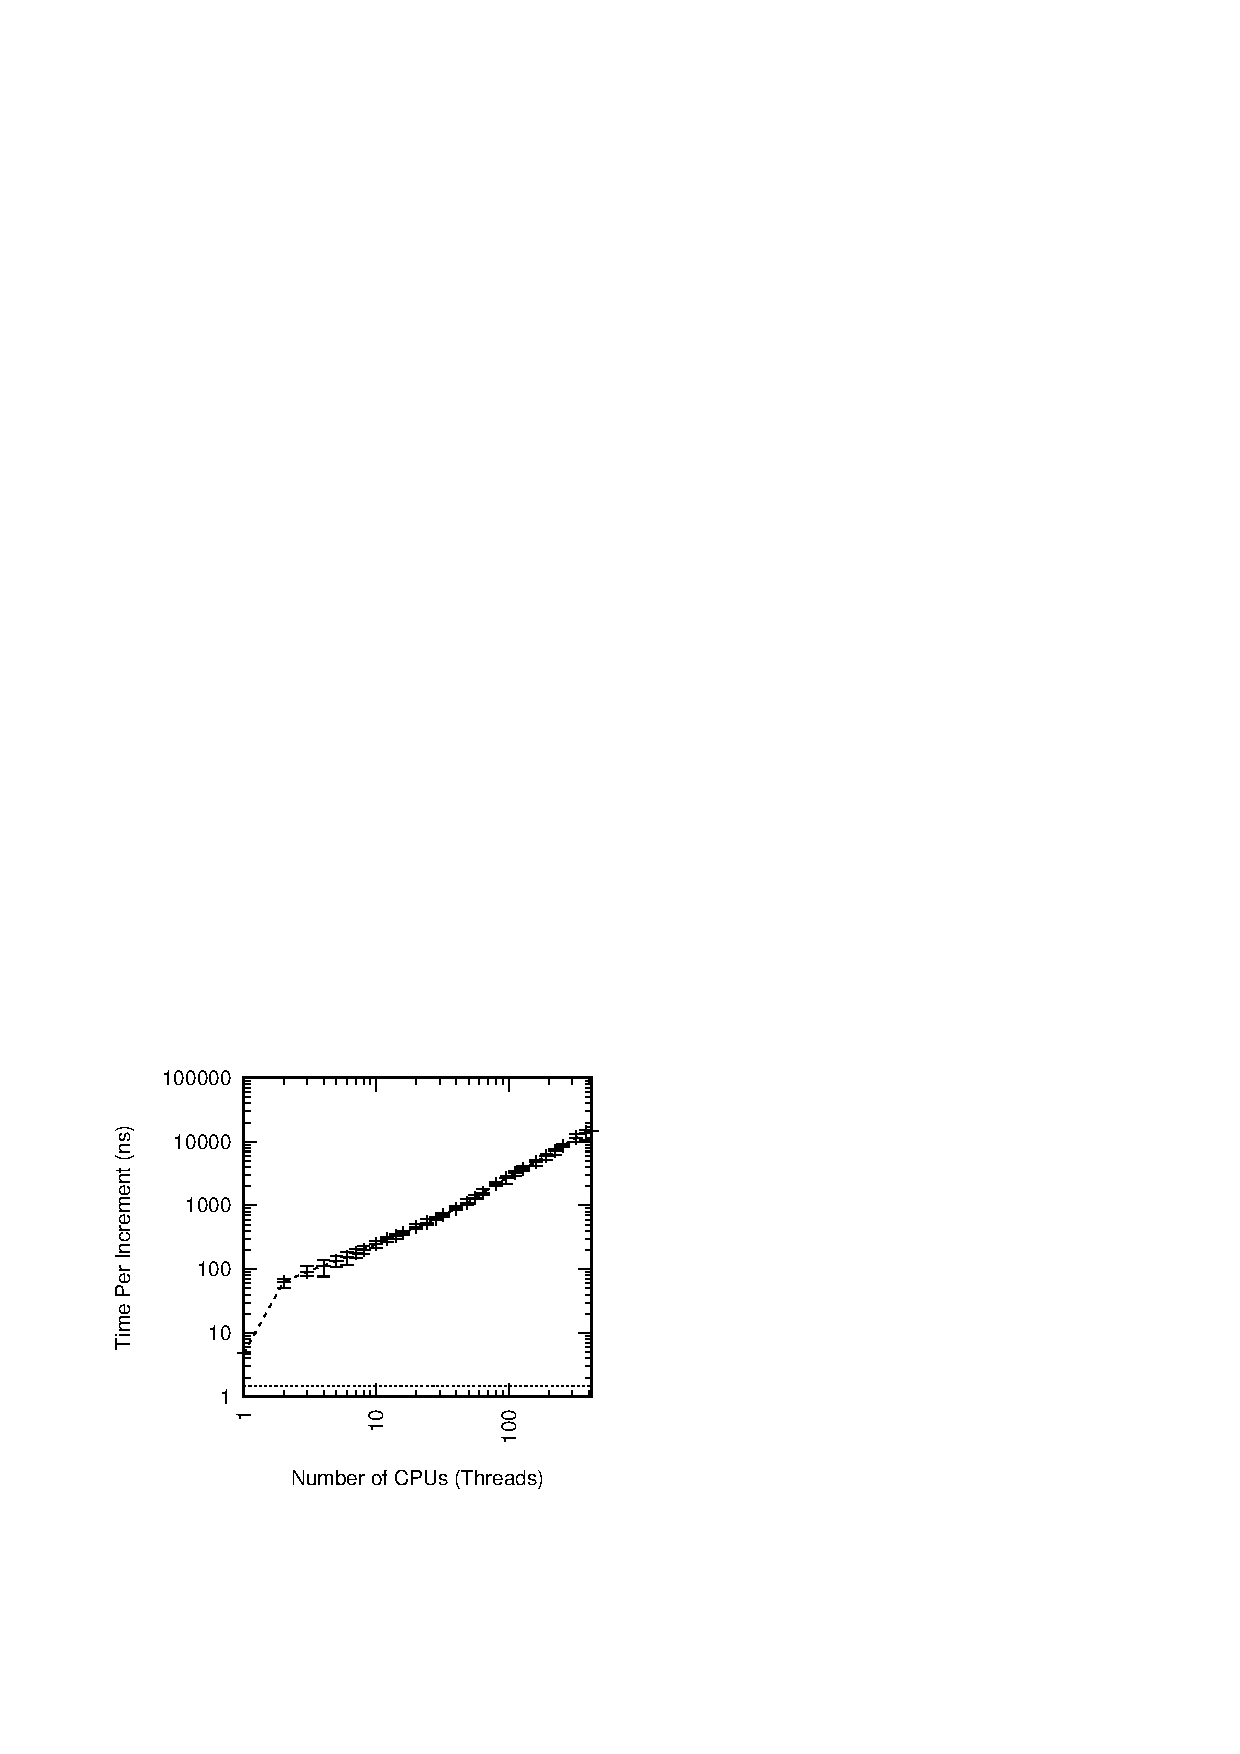
\includegraphics{CodeSamples/count/atomic_hps.pdf}}
\caption{Atomic Increment Scalability on x86}
\label{fig:count:Atomic Increment Scalability on x86}
\end{figure}

정확한 카운팅을 하는 간단한 방법은
Listing~\ref{lst:count:Just Count Atomically!} (\path{count_atomic.c})
에 보여진 것처럼 어토믹 오퍼레이션을 사용하는 것입니다.
\begin{fcvref}[ln:count:count_atomic:inc-read]
라인~\lnref{counter} 는 어토믹 변수를 정의하고, 라인~\lnref{inc} 는 이를
어토믹하게 증가시키며, 라인~\lnref{read} 는 이를 읽습니다.
\end{fcvref}
이것은 어토믹 하므로, 완전한 카운트를 유지합니다.
하지만, 더 느립니다: 제 6개 코어 x86 랩톱에서, 어토믹하지 않은 값 증가 버전에
비해, 단일 쓰레드만 사용될 때 조차도 20배가 넘게 느립니다.\footnote{
	흥미롭게도, 어토믹하지 않게 카운터를 증가시키는 것은 어토믹하게 이
	카운터를 증가시키는 것보다도 빠른 속도로 그 값을 증가시킵니다.
	물론, 여러분의 목표가 오직 이 카운터를 빨리 증가시키려는 거라면, 더
	쉬운 방법은 그냥 큰 값을 이 카운터에 할당하는 것일 겁니다.
	하지만, 더 큰 성능과 확장성을 위해 완화된 정확성의 개념을 주의 깊게
	사용하는 알고리즘의 역할도 있을 수 있을
	겁니다~\cite{Andrews91textbook,Arcangeli03,10.5555/3241639.3241645,DavidUngar2011unsync}.}

\iffalse

The straightforward way to count accurately is to use atomic operations,
as shown in
Listing~\ref{lst:count:Just Count Atomically!} (\path{count_atomic.c}).
\begin{fcvref}[ln:count:count_atomic:inc-read]
Line~\lnref{counter} defines an atomic variable,
line~\lnref{inc} atomically increments it, and
line~\lnref{read} reads it out.
\end{fcvref}
Because this is atomic, it keeps perfect count.
However, it is slower: on my six-core x86 laptop, it is more than
twenty times slower than non-atomic increment, even
when only a single thread is incrementing.\footnote{
	Interestingly enough, non-atomically incrementing a counter will
	advance the counter more quickly than atomically incrementing
	the counter.
	Of course, if your only goal is to make the counter increase
	quickly, an easier approach is to simply assign a large value
	to the counter.
	Nevertheless, there is likely to be a role for algorithms that
	use carefully relaxed notions of correctness in order to gain
	greater performance and
	scalability~\cite{Andrews91textbook,Arcangeli03,10.5555/3241639.3241645,DavidUngar2011unsync}.}

\fi

이 처참한 성능은
Chapter~\ref{chp:Hardware and its Habits}
에서의 토의를 생각해 보면 놀랍지 않은 것이고, 어토믹 값 증가의 성능이 CPU 와
쓰레드의 수가 증가함에 따라
Figure~\ref{fig:count:Atomic Increment Scalability on x86}
에 보여진 것처럼 더 느려지는 것도 놀라운 일이 아닙니다.
이 그림에서, x~축의 가로로 그려진 점선은 완전하게 확장되는 알고리즘이 얻을 수
있을 이상적 성능입니다: 그런 알고리즘이 있다면, 하나의 값 증가는 싱글쓰레드
프로그램에서의 것과 동일한 오버헤드만을 일으킬 겁니다.
단일 전역 변수의 어토믹 값 증가는 분명 이상적이지 않고, 추가되는 CPU 에서
수천수만배의 오버헤드를 일으킵니다.

\iffalse

This poor performance should not be a surprise, given the discussion in
Chapter~\ref{chp:Hardware and its Habits},
nor should it be a surprise that the performance of atomic increment
gets slower as the number of CPUs and threads increase, as shown in
Figure~\ref{fig:count:Atomic Increment Scalability on x86}.
In this figure, the horizontal dashed line resting on the x~axis
is the ideal performance that would be achieved
by a perfectly scalable algorithm: with such an algorithm, a given
increment would incur the same overhead that it would in a single-threaded
program.
Atomic increment of a single global variable is clearly
decidedly non-ideal, and gets multiple orders of magnitude worse with
additional CPUs.

\fi

\QuickQuizSeries{%
\QuickQuizB{
	x~축 상의 가로의 점선은 왜 $x=1$ 에서 대각선에 붙지 않나요?

	\iffalse

	Why doesn't the horizontal dashed line on the x~axis meet the
	diagonal line at $x=1$?

	\fi

}\QuickQuizAnswerB{
	어토믹 오퍼레이션의 오버헤드 때문입니다.
	x~축 상의 점선은 단일 \emph{non-atomic} 값 증가의 오버헤드를
	나타냅니다.
	어쨌건, \emph{이상적인} 알고리즘은 선형으로 확장하기만 하는게 아니라,
	싱글쓰레드 코드에 비교해서도 성능 페널티를 일으키지 않을 겁니다.

	이 수준의 이상성은 지나치게 느껴질 수도 있겠으나, 이게
	\ppl{Linus}{Torvalds} 에게 충분히 좋다면, 여러분에게도 충분히 좋을
	겁니다.

	\iffalse

	Because of the overhead of the atomic operation.
	The dashed line on the x~axis represents the overhead of
	a single \emph{non-atomic} increment.
	After all, an \emph{ideal} algorithm would not only scale
	linearly, it would also incur no performance penalty compared
	to single-threaded code.

	This level of idealism may seem severe, but if it is good
	enough for \ppl{Linus}{Torvalds}, it is good enough for you.

	\fi

}\QuickQuizEndB
%
\QuickQuizE{
	하지만 어토믹 값 증가는 여전히 무척 빠릅니다.
	그리고 짧은 반복문 내에서 하나의 변수를 값 증가시키는 것은 제게 굉장히
	비현실적으로 들리는데, 어쨌건, 대부분의 프로그램의 실행은 진짜 일을
	하는데 사용되어야지, 자신이 한 일을 세는데 쓰이면 안됩니다!
	왜 제가 이걸 빠르게 하는데 신경을 써야 하죠?

	\iffalse

	But atomic increment is still pretty fast.
	And incrementing a single variable in a tight loop sounds
	pretty unrealistic to me, after all, most of the program's
	execution should be devoted to actually doing work, not accounting
	for the work it has done!
	Why should I care about making this go faster?

	\fi

}\QuickQuizAnswerE{
	많은 경우에, 어토믹 값 증가는 실제로 여러분에게 충분히 빠를 겁니다.
	그런 경우에, 여러분은 어토믹 값 증가를 사용해야 합니다.
	그러나, 더 나은 카운팅 알고리즘이 필요한 실제 세계의 상황들이 많이
	있습니다.
	그런 상황의 예 중 하나는 상당히 최적화 된 네트워킹 스택에서 패킷과
	바이트를 세는 것으로, 특히 거대한 멀티프로세서에서라면 이런 종류의
	카운팅 작업에 상당히 많은 수행 시간이 사용되기 쉽습니다.

	또한, 이 챕터의 시작에서 이야기 했듯이, 카운팅은 공유 메모리 병렬
	프로그램에서 마주칠 수 있는 문제들을 잘 보여줍니다.

	\iffalse

	In many cases, atomic increment will in fact be fast enough
	for you.
	In those cases, you should by all means use atomic increment.
	That said, there are many real-world situations where
	more elaborate counting algorithms are required.
	The canonical example of such a situation is counting packets
	and bytes in highly optimized networking stacks, where it is
	all too easy to find much of the execution time going into
	these sorts of accounting tasks, especially on large
	multiprocessors.

	In addition, as noted at the beginning of this chapter,
	counting provides an excellent view of the
	issues encountered in shared-memory parallel programs.

	\fi

}\QuickQuizEndE
}

\begin{figure}[tb]
\centering
\resizebox{3in}{!}{\includegraphics{count/GlobalInc}}
\caption{Data Flow For Global Atomic Increment}
\label{fig:count:Data Flow For Global Atomic Increment}
\end{figure}

\begin{figure}[tb]
\centering
\resizebox{3.2in}{!}{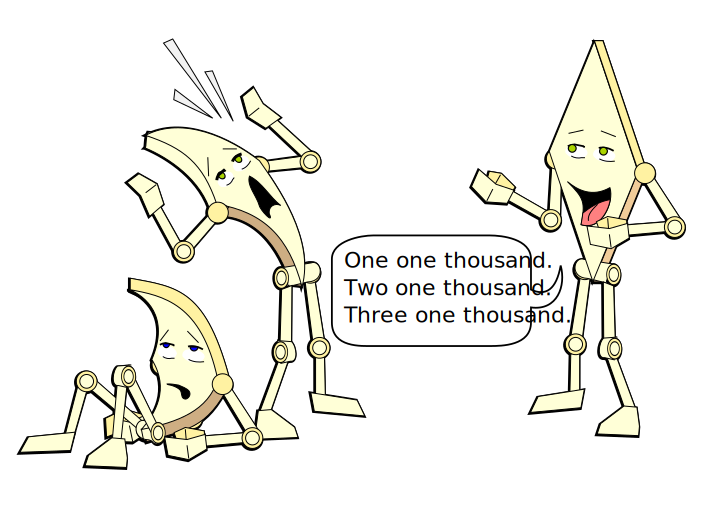
\includegraphics{cartoons/r-2014-One-one-thousand}}
\caption{Waiting to Count}
\ContributedBy{Figure}{fig:count:Waiting to Count}{Melissa Broussard}
\end{figure}

전역 어토믹 값 증가에 대한 다른 관점을 위해,
Figure~\ref{fig:count:Data Flow For Global Atomic Increment}
를 보시기 바랍니다.
각 CPU 가 주어진 전역 변수의 값을 증가할 기회를 얻기 위해, 해당 변수를 담고
있는 캐쉬 라인은 빨간 화살표로 보여진 것처럼 모든 CPU 사이를 순환해야만 합니다.
그런 순환은 상당한 시간을 취할 것이어서,
Figure~\ref{fig:count:Atomic Increment Scalability on x86}
에 보여진 처참한 성능에 이를 것으로,
Figure~\ref{fig:count:Waiting to Count}
처럼 생각될 수 있겠습니다.
다음 섹션들에서는 이런 순환에서 피할 수 없는 지연을 회피하기 위한 고성능
카운팅에 대해 이야기 해봅니다.

\iffalse

For another perspective on global atomic increment, consider
Figure~\ref{fig:count:Data Flow For Global Atomic Increment}.
In order for each CPU to get a chance to increment a given
global variable, the cache line containing that variable must
circulate among all the CPUs, as shown by the red arrows.
Such circulation will take significant time, resulting in
the poor performance seen in
Figure~\ref{fig:count:Atomic Increment Scalability on x86},
which might be thought of as shown in
Figure~\ref{fig:count:Waiting to Count}.
The following sections discuss high-performance counting, which
avoids the delays inherent in such circulation.

\fi

\QuickQuiz{
	하지만 왜 CPU 설계자들은 값이 증가되어야 하는 전역 변수를 담고 있는
	캐쉬 라인이 순환될 필요를 없애는 추가적인 기능을 제공하지 않는 거죠?

	\iffalse

	But why can't CPU designers simply ship the addition operation to the
	data, avoiding the need to circulate the cache line containing
	the global variable being incremented?

	\fi

}\QuickQuizAnswer{
	어떤 경우들에는 그렇게 하는게 가능할 수도 있습니다.
	하지만, 좀 복잡한 부분이 있습니다:
	\begin{enumerate}
	\item	이 변수의 값이 필요하다면, 이 쓰레드는 이 오퍼레이션이 이
		데이터에 도달할 때까지, 그리고 나서는 그 결과가 돌아올 때까지
		기다려야 합니다.
	\item	이 어토믹 값 증가가 앞 또는 뒤의 오퍼레이션들에 대해
		순서지어져야 한다면, 이 쓰레드는 이 오퍼레이션이 이 데이터에
		도달할 때까지, 그리고 이 오퍼레이션이 완료되었다는 통지가
		돌아올 때까지 기다려야 합니다.
	\item	CPU 들 사이에서 오퍼레이션을 전달하는 것은 시스템 인터커넥트
		상에 더 많은 선로를 필요로 할텐데, 이는 더 많은 다이 영역과
		전력을 소모할 겁니다.
	\end{enumerate}
	하지만 첫번째 두 조건들이 없다면 어떨까요?
	그렇다면 여러분은 평범한 하드웨어에서 이상에 가까운 성능을 달성하는,
	Section~\ref{sec:count:Statistical Counters}
	에서 이야기 하는 알고리즘을 주의 깊게 생각해 봐야 합니다.

	\iffalse

	It might well be possible to do this in some cases.
	However, there are a few complications:
	\begin{enumerate}
	\item	If the value of the variable is required, then the
		thread will be forced to wait for the operation
		to be shipped to the data, and then for the result
		to be shipped back.
	\item	If the atomic increment must be ordered with respect
		to prior and/or subsequent operations, then the thread
		will be forced to wait for the operation to be shipped
		to the data, and for an indication that the operation
		completed to be shipped back.
	\item	Shipping operations among CPUs will likely require
		more lines in the system interconnect, which will consume
		more die area and more electrical power.
	\end{enumerate}
	But what if neither of the first two conditions holds?
	Then you should think carefully about the algorithms discussed
	in Section~\ref{sec:count:Statistical Counters}, which achieve
	near-ideal performance on commodity hardware.

	\fi

\begin{figure}[tb]
\centering
\resizebox{3in}{!}{\includegraphics{count/GlobalTreeInc}}
\caption{Data Flow For Global Combining-Tree Atomic Increment}
\label{fig:count:Data Flow For Global Combining-Tree Atomic Increment}
\end{figure}

	앞의 두 조건 중 하나라도 성립된다면, 개선된 하드웨어를 위한 \emph{어떤}
	희망이 있습니다.
	하드웨어가 콤바이닝 트리를 구현해서 여러 CPU 로부터의 값 증가 요청이
	하드웨어에 의해 하나의 값 추가로 결합되는 걸 상상해 볼 수 있겠습니다.
	이 하드웨어는 또한 이 요청들에 순서를 적용시켜서, 각 CPU 에게 각자의
	어토믹 값 증가에 해당하는 값을 리턴시켜줄 수도 있을 겁니다.
	이는 이 명령의 응답시간을 $\O{\log N}$ 으로 만들텐데, $N$ 은
	Figure~\ref{fig:count:Data Flow For Global Combining-Tree Atomic Increment}
	에 보인 것과 같이 CPU 갯수입니다.
	그리고 이런 종류의 하드웨어 최적화를 가진 CPU 들이 2011년부터 등장하기
	시작했습니다.

	이는
	Figure~\ref{fig:count:Data Flow For Global Atomic Increment}
	에 보인 현재 하드웨어의 $\O{N}$ 성능에 비해 엄청난 개선이며, 3차원 구조
	같은 혁신이 실용적인 것으로 증명된다면 추가적인 하드웨어 응답시간
	감소도 가능합니다.
	그러나, 어떤 중요한 특수한 경우에 있어서는 소프트웨어가 \emph{훨씬} 잘
	할 수 있음을 볼 겁니다.

	\iffalse

	If either or both of the first two conditions hold, there is
	\emph{some} hope for improved hardware.
	One could imagine the hardware implementing a combining tree,
	so that the increment requests from multiple CPUs are combined
	by the hardware into a single addition when the combined request
	reaches the hardware.
	The hardware could also apply an order to the requests, thus
	returning to each CPU the return value corresponding to its
	particular atomic increment.
	This results in instruction latency that varies as $\O{\log N}$,
	where $N$ is the number of CPUs, as shown in
	Figure~\ref{fig:count:Data Flow For Global Combining-Tree Atomic Increment}.
	And CPUs with this sort of hardware optimization started to
	appear in 2011.

	This is a great improvement over the $\O{N}$ performance
	of current hardware shown in
	Figure~\ref{fig:count:Data Flow For Global Atomic Increment},
	and it is possible that hardware latencies might decrease
	further if innovations such as three-dimensional fabrication prove
	practical.
	Nevertheless, we will see that in some important special cases,
	software can do \emph{much} better.

	\fi

}\QuickQuizEnd

\section{Statistical Counters}
\label{sec:count:Statistical Counters}
%
\epigraph{Facts are stubborn things, but statistics are pliable.}
	 {\emph{Mark Twain}}

이 섹션은 카운트가 무척 자주 업데이트 되고 그 값은 가끔만 읽혀지는, 통계적
카운터라는 흔한 구체적 케이스를 다룹니다.
이는 \QuickQuizRef{\QcountQstatcnt} 에서 암시된 네트워크 패킷 카운팅 문제를
푸는데 사용될 겁니다.

\iffalse

This section covers the common special case of statistical counters, where
the count is updated extremely frequently and the value is read out
rarely, if ever.
These will be used to solve the network-packet counting problem
posed in \QuickQuizRef{\QcountQstatcnt}.

\fi

\subsection{Design}

통계적 카운팅은 일반적으로 쓰레드당 (또는 커널에서 돌아가는 경우라면 CPU 당)
카운터를 제공해서
page~\pageref{sec:toolsoftrade:Per-CPU Variables} 의
Section~\ref{sec:toolsoftrade:Per-CPU Variables}
에서 앞서 보여진 것처럼 각 쓰레드가 자신의 카운터를 증가시키도록 합니다.
카운터들의 합쳐진 값은 간단히 이 쓰레드들의 카운터를 모두 합해서 구해지는데,
더하기의 상호성과 결합성에 의존합니다.
이는
page~\pageref{sec:SMPdesign:Data Ownership} 의
Section~\ref{sec:SMPdesign:Data Ownership}
에서 소개된 데이터 소유권 패턴의 한 예입니다.

\iffalse

Statistical counting is typically handled by providing a counter per
thread (or CPU, when running in the kernel), so that each thread
updates its own counter, as was foreshadowed in
Section~\ref{sec:toolsoftrade:Per-CPU Variables}
on page~\pageref{sec:toolsoftrade:Per-CPU Variables}.
The aggregate value of the counters is read out by simply summing up
all of the threads' counters,
relying on the commutative and associative properties of addition.
This is an example of the Data Ownership pattern that will be introduced in
Section~\ref{sec:SMPdesign:Data Ownership}
on page~\pageref{sec:SMPdesign:Data Ownership}.

\fi

\QuickQuiz{
	하지만 C 의 ``정수형'' 이 크기 제한이 있다는 사실이 이를 복잡하게
	만들지는 않나요?

	\iffalse

	But doesn't the fact that C's ``integers'' are limited in size
	complicate things?

	\fi

}\QuickQuizAnswer{
	아닙니다, 왜냐하면 더하기는 여전히 상호적이고 결합적입니까요.
	최소한 unsigned integer 를 사용하는 동안은요.
	C 표준에서, signed integer 의 오버플로우는 undefined behavior 를
	초래함을 기억하시고, 오버플로우 시에 래핑 외의 어떤 일을 하는 기계는
	요즘 굉장히 드물다는 사실은 신경쓰지 마세요.
	불행히도, 컴파일러는 signed integer 가 절대 오버플로우 되지 않을 거라는
	가정 하에 최적화를 종종 행하여서, 여러분의 코드가 signed integer 를
	오버플로우 나게 한다면, 현대의 twos-complement 하드웨어에서라도 문제를
	일으킬 수 있습니다.

	그렇다고는 하나, (예를 들어) 32비트 쓰레드당 카운터의 합을 64비트로
	만들려 할 때 추가적인 복잡도의 요인이 존재합니다.
	이런 추가적 복잡성을 처리하는 것은 독자 여러분의 몫으로 남겨두겠는데,
	이 챕터의 뒷부분에서 소개되는 일부 기법들이 상당히 도움이 될 겁니다.

	\iffalse

	No, because modulo addition is still commutative and associative.
	At least as long as you use unsigned integers.
	Recall that in the C standard, overflow of signed integers results
	in undefined behavior, never mind the fact that machines that
	do anything other than wrap on overflow are quite rare these days.
	Unfortunately, compilers frequently carry out optimizations that
	assume that signed integers will not overflow, so if your code
	allows signed integers to overflow, you can run into trouble
	even on modern twos-complement hardware.

	That said, one potential source of additional complexity arises
	when attempting to gather (say) a 64-bit sum from 32-bit
	per-thread counters.
	Dealing with this added complexity is left as
	an exercise for the reader, for whom some of the techniques
	introduced later in this chapter could be quite helpful.

	\fi

}\QuickQuizEnd

\subsection{Array-Based Implementation}
\label{sec:count:Array-Based Implementation}

쓰레드당 변수를 제공하는 한가지 방법은 (거짓 공유를 방지하기 위해 캐쉬라인에
맞춰 정렬되고 패딩 되어 있다는 가정 하에) 쓰레드당 하나의 원소를 갖는 배열을
할당하는 것입니다.

\iffalse

One way to provide per-thread variables is to allocate an array with
one element per
thread (presumably cache aligned and padded to avoid false sharing).

\fi

\QuickQuiz{
	배열이요???
	하지만 그럼 쓰레드의 수가 제한되지 않나요?

	\iffalse

	An array???
	But doesn't that limit the number of threads?

	\fi

}\QuickQuizAnswer{
	그럴 수 있습니다, 그리고 이 장난감 구현에서는, 그렇습니다.
	하지만 임의의 수의 쓰레드를 허용하는 대안적 구현은 그렇게 어렵지
	않은데, 예를 들면
	Section~\ref{sec:count:Per-Thread-Variable-Based Implementation}
	에 보여진 \GCC 의 \co{__thread} 기능을 사용하는 겁니다.

	\iffalse

	It can, and in this toy implementation, it does.
	But it is not that hard to come up with an alternative
	implementation that permits an arbitrary number of threads,
	for example, using \GCC's \co{__thread} facility,
	as shown in
	Section~\ref{sec:count:Per-Thread-Variable-Based Implementation}.

	\fi

}\QuickQuizEnd

\begin{listing}[tbp]
\input{CodeSamples/count/count_stat@inc-read.fcv}
\caption{Array-Based Per-Thread Statistical Counters}
\label{lst:count:Array-Based Per-Thread Statistical Counters}
\end{listing}

그런 배열은
Listing~\ref{lst:count:Array-Based Per-Thread Statistical Counters}
(\path{count_stat.c})
에 보여진 per-thread 기능으로 감싸질 수 있습니다.
\begin{fcvref}[ln:count:count_stat:inc-read]
라인~\lnref{define} 은 창의적이게도 \co{counter} 라고 이름지어진, \co{unsigned
long} 타입의 쓰레드당 카운터의 집합을 담는 배열을 정의합니다.

\Clnrefrange{inc:b}{inc:e} 는 \co{__get_thread_var()} 기능을 현재 수행중인
쓰레드의 \co{counter} 배열 내 원소 위치를 알아내기 위해 사용해서 카운터를
증가시키는 함수를 보입니다.
이 원소는 이 연관된 쓰레드에 의해서만 증가되므로, 어토믹하지 않은 값 증가로도
충분합니다.
하지만, 이 코드는 위험한 컴파일러 최적화를 방지하기 위해 \co{WRITE_ONCE()} 를
사용합니다.
한가지 예만 들자면, 이 컴파일러는 저장되어질 위치를 임시의 저장소로 사용할
권리를 갖고 있으므로, 이 위치에 어떤 의도와 목적으로든 쓰레기를 이 요청된
스토어 이전에 이 위치에 저장할 수 있습니다.
이는 당연하게도 이 카운트를 읽으려는 모든 시도를 혼란하게 만들 수 있습니다.
\co{WRITE_ONCE()} 의 사용은 이 최적화와 다른 것들을 방지해 줍니다.

\iffalse

Such an array can be wrapped into per-thread primitives, as shown in
Listing~\ref{lst:count:Array-Based Per-Thread Statistical Counters}
(\path{count_stat.c}).
\begin{fcvref}[ln:count:count_stat:inc-read]
Line~\lnref{define} defines an array containing a set of per-thread counters of
type \co{unsigned long} named, creatively enough, \co{counter}.

\Clnrefrange{inc:b}{inc:e}
show a function that increments the counters, using the
\co{__get_thread_var()} primitive to locate the currently running
thread's element of the \co{counter} array.
Because this element is modified only by the corresponding thread,
non-atomic increment suffices.
However, this code uses \co{WRITE_ONCE()} to prevent destructive compiler
optimizations.
For but one example, the compiler is within its rights to use a
to-be-stored-to location as temporary storage, thus writing what
would be for all intents and purposes garbage to that location
just before doing the desired store.
This could of course be rather confusing to anything attempting to
read out the count.
The use of \co{WRITE_ONCE()} prevents this optimization and others besides.

\fi

\QuickQuiz{
	\GCC\ 는 이것 외에 어떤 못된 최적화를 할 수 있나요?

	\iffalse

	What other nasty optimizations could \GCC\ apply?

	\fi
}\QuickQuizAnswer{
	더 많은 정보를 위해
	\cref{sec:toolsoftrade:Shared-Variable Shenanigans,%
	sec:memorder:Compile-Time Consternation}
	를 참고하시기 바랍니다.
	한가지 못된 최적화는 뒤따르는 \co{read_count()} 함수에 흔한 부가적 표현
	제거를 적용하는 것으로, 이는 이 값의 변화가 이 함수로의 이어지는
	호출로부터 리턴될 거라고 믿는 코드를 놀라게 할 수도 있을 겁니다.

	\iffalse

	See \cref{sec:toolsoftrade:Shared-Variable Shenanigans,%
	sec:memorder:Compile-Time Consternation}
	for more information.
	One nasty optimization would be to apply common subexpression
	elimination to successive calls to the \co{read_count()} function,
	which might come as a surprise to code expecting changes in the
	values returned from successive calls to that function.

	\fi

}\QuickQuizEnd

\Clnrefrange{read:b}{read:e}
는 이 카운터의 합쳐진 값을 읽어들이는데, 현재 수행중인 쓰레드의 리스트를
순회하는데에 \co{for_each_thread()} 기능을 사용하고, 특정 쓰레드의 카운터를
읽어들이기 위해 \co{per_thread()} 기능을 사용합니다.
이 코드는 또한 컴파일러가 이 로드를 무시하는 최적화를 하지 못하게
\co{READ_ONCE()} 를 사용합니다.
한가지만 예를 들자면, \co{read_count()} 로의 이어지는 두개의 호출은 인라인될
수도 있고, 대담한 최적화는 같은 위치가 더하기 되었으며 따라서 이것들을 한번만
더하기 하고 그 결과 값을 두번 사용하는게 더 간단하고 나을 수 있을 거라는 잘못된
결론을 내릴 수 있습니다.
이런 종류의 최적화는 나중의 \co{read_count()} 호출이 다른 쓰레드의 활동을
계산할 거라 예상하는 사람들을 좌절하게 만들 수도 있습니다.
\co{READ_ONCE()} 의 사용은 이 최적화와 비슷한 것들을 방지합니다.
\end{fcvref}

\iffalse

\Clnrefrange{read:b}{read:e}
show a function that reads out the aggregate value of the counter,
using the \co{for_each_thread()} primitive to iterate over the list of
currently running threads, and using the \co{per_thread()} primitive
to fetch the specified thread's counter.
This code also uses \co{READ_ONCE()} to ensure that the compiler doesn't
optimize these loads into oblivion.
For but one example, a pair of consecutive calls to \co{read_count()}
might be inlined, and an intrepid optimizer might notice that the same
locations were being summed and thus incorrectly conclude that it would
be simply wonderful to sum them once and use the resulting value twice.
This sort of optimization might be rather frustrating to people expecting
later \co{read_count()} calls to account for the activities of other
threads.
The use of \co{READ_ONCE()} prevents this optimization and others besides.
\end{fcvref}

\fi

\QuickQuizSeries{%
\QuickQuizB{
	Listing~\ref{lst:count:Array-Based Per-Thread Statistical Counters}
	의 \co{counter} per-thread 변수는 어떻게 초기화 되나요?

	\iffalse

	How does the per-thread \co{counter} variable in
	Listing~\ref{lst:count:Array-Based Per-Thread Statistical Counters}
	get initialized?

	\fi

}\QuickQuizAnswerB{
	C 표준은 전역 변수의 초기값은 명시적으로 초기화 되지 않는다면 0이라고
	명시하고 있으므로, \co{counter} 의 모든 인스턴스는 묵시적으로 0으로
	초기화 됩니다.
	이와는 별개로, 사용자가 통계적 카운터들로부터의 연속된 읽기 사이의
	차이에 대해서만 관심이 있다면 이 초기값은 의미 없을 겁니다.

	\iffalse

	The C standard specifies that the initial value of
	global variables is zero, unless they are explicitly initialized,
	thus implicitly initializing all the instances of \co{counter}
	to zero.
	Besides, in the common case where the user is interested only in
	differences between consecutive reads from statistical counters,
	the initial value is irrelevant.

	\fi

}\QuickQuizEndB
%
\QuickQuizE{
	Listing~\ref{lst:count:Array-Based Per-Thread Statistical Counters}
	의 코드는 복수의 카운터를 어떻게 허용할까요?

	\iffalse

	How is the code in
	Listing~\ref{lst:count:Array-Based Per-Thread Statistical Counters}
	supposed to permit more than one counter?

	\fi

}\QuickQuizAnswerE{
	실제로, 이 장난감 예제는 복수의 카운터를 허용하지 않습니다.
	복수의 카운터를 제공할 수 있도록 이걸 수정하는 것은 독자 여러분의
	과제로 남겨둡니다.

	\iffalse

	Indeed, this toy example does not support more than one counter.
	Modifying it so that it can provide multiple counters is left
	as an exercise to the reader.

	\fi

}\QuickQuizEndE
}

\begin{figure}[tb]
\centering
\resizebox{3in}{!}{\includegraphics{count/PerThreadInc}}
\caption{Data Flow For Per-Thread Increment}
\label{fig:count:Data Flow For Per-Thread Increment}
\end{figure}

이 방법은 \co{inc_count()} 를 수행하는 업데이트 쓰레드의 수의 증가와 함께
선형적으로 확장됩니다.
Figure~\ref{fig:count:Data Flow For Per-Thread Increment}
의 각 CPU 에 초록 화살표로 보여진 것처럼, 이에 대한 이유는 각 CPU 가 비싼
시스템간 통신 없이 자신의 쓰레드의 변수를 값 증가시키는데 빠른 진행을 만든다는
것입니다.
그것으로서, 이 섹션은 이 챕터의 시작에서 이야기 된 네트워크 패킷 카운팅 문제를
해결합니다.

\iffalse

This approach scales linearly with increasing number of updater threads
invoking \co{inc_count()}.
As is shown by the green arrows on each CPU in
Figure~\ref{fig:count:Data Flow For Per-Thread Increment},
the reason for this is that each CPU can make rapid progress incrementing
its thread's variable, without any expensive cross-system communication.
As such, this section solves the network-packet counting problem presented
at the beginning of this chapter.

\fi

\QuickQuiz{
	이 읽기 오퍼레이션은 쓰레드당 값을 합하는데 시간을 요하며, 이 시간 동안
	이 카운터의 값은 변화될 수 있습니다.
	이는
	Listing~\ref{lst:count:Array-Based Per-Thread Statistical Counters}
	의 \co{read_count()} 를 통해 리턴되는 값은 정확하지 않을 것을
	의미합니다.
	이 카운터는 단위 시간당 $r$ 카운트의 속도로 증가된다고, 그리고
	\co{read_count()} 의 수행은 $\Delta$ 단위 시간을 소모한다고 가정해
	봅시다.
	리턴되는 값에 예상되는 에러는 얼마정도일까요?

	\iffalse

	The read operation takes time to sum up the per-thread values,
	and during that time, the counter could well be changing.
	This means that the value returned by
	\co{read_count()} in
	Listing~\ref{lst:count:Array-Based Per-Thread Statistical Counters}
	will not necessarily be exact.
	Assume that the counter is being incremented at rate
	$r$ counts per unit time, and that \co{read_count()}'s
	execution consumes $\Delta$ units of time.
	What is the expected error in the return value?

	\fi

}\QuickQuizAnswer{
	최악의 경우에 대한 분석을 먼저 하고, 이어서 덜 보수적인 분석을
	해봅시다.

	최악의 경우, 읽기 오퍼레이션은 순식간에 완료되지만, 리턴하기 전에
	$\Delta$ 시간의 지연을 가져서, 최악의 경우의 에러는 단순히 $r \Delta$
	가 됩니다.

	이 최악의 경우 행동은 가능성이 적으므로, $N$ 개의 카운터 각각으로부터의
	읽기가 $\Delta$ 시간 동안 동일한 시간을 사용한다고 생각해 봅시다.
	$N$ 개의 읽기 사이에는 $\frac{\Delta}{N+1}$ 시간의 $N+1$ 개 시간 간격이
	존재할 겁니다.
	마지막 쓰레드의 카운터로부터의 읽기 이후의 이 지연으로 인한 에러는 
	$\frac{r \Delta}{N \left( N + 1 \right)}$ 이 될 것이며, 뒤에서 두번째
	쓰레드의 카운터로부터의 에러는
	$\frac{2 r \Delta}{N \left( N + 1 \right)}$,
	뒤에서 세번째 쓰레드는
	$\frac{3 r \Delta}{N \left( N + 1 \right)}$,
	이런 식으로 될 겁니다.
	총 에러는 각 쓰레드의 카운터로부터의 읽기로 인한 에러들의 합이 되므로:

	\iffalse

	Let's do worst-case analysis first, followed by a less
	conservative analysis.

	In the worst case, the read operation completes immediately,
	but is then delayed for $\Delta$ time units before returning,
	in which case the worst-case error is simply $r \Delta$.

	This worst-case behavior is rather unlikely, so let us instead
	consider the case where the reads from each of the $N$
	counters is spaced equally over the time period $\Delta$.
	There will be $N+1$ intervals of duration $\frac{\Delta}{N+1}$
	between the $N$ reads.
	The error due to the delay after the read from the last thread's
	counter will be given by $\frac{r \Delta}{N \left( N + 1 \right)}$,
	the second-to-last thread's counter by
	$\frac{2 r \Delta}{N \left( N + 1 \right)}$,
	the third-to-last by
	$\frac{3 r \Delta}{N \left( N + 1 \right)}$,
	and so on.
	The total error is given by the sum of the errors due to the
	reads from each thread's counter, which is:

	\fi

	\begin{equation}
		\frac{r \Delta}{N \left( N + 1 \right)}
			\sum_{i = 1}^N i
	\end{equation}

	이 합을 닫힌 형태로 정리해 보면:

	\iffalse

	Expressing the summation in closed form yields:

	\fi

	\begin{equation}
		\frac{r \Delta}{N \left( N + 1 \right)}
			\frac{N \left( N + 1 \right)}{2}
	\end{equation}

	중복을 제거하면 다음과 같이 직관적으로 예상된 결과가 나옵니다:

	\iffalse

	Canceling yields the intuitively expected result:

	\fi

	\begin{equation}
		\frac{r \Delta}{2}
	\label{eq:count:CounterErrorAverage}
	\end{equation}

	호출자가 이 읽기 오퍼레이션을 통해 리턴된 카운트를 사용하는 코드를
	수행하는 동안에도 이 에러는 증가함을 기억해 두는 것이 중요합니다.
	예를 들어, 리턴된 카운트의 값에 기반한 어떤 계산을 수행하는 데에 $t$
	시간을 소모했다면, 최악의 경우의 에러는 $r \left(\Delta + t\right)$ 로
	증가할 겁니다.

	예상되는 에러 역시 비슷하게 다음과 같이 증가합니다:

	\iffalse

	It is important to remember that error continues accumulating
	as the caller executes code making use of the count returned
	by the read operation.
	For example, if the caller spends time $t$ executing some
	computation based on the result of the returned count, the
	worst-case error will have increased to $r \left(\Delta + t\right)$.

	The expected error will have similarly increased to:

	\fi

	\begin{equation}
		r \left( \frac{\Delta}{2} + t \right)
	\end{equation}

	물론, 어떤 경우에는 읽기 오퍼레이션 동안 카운터의 값이 계속 증가하는게
	받아들여질 수 없을 때도 있습니다.
	Section~\ref{sec:count:Applying Exact Limit Counters}
	은 이 상황을 처리하는 방법을 이야기 합니다.

	지금까지, 우리는 값이 증가하기만 하지 감소하지는 않는 카운터를 생각해
	봤습니다.
	만약 이 카운터 값이 단위 시간당 $r$ 카운트 만큼만 바뀌지만, 어떤
	방향에서든 그렇다면, 우린 이 에러가 줄어들 것이라고 예상해야 합니다.
	하지만, 최악의 경우는 카운터가 양방향으로 움직일 수 \emph{있다고} 해도
	이 최악의 경우는 읽기 오퍼레이션이 순식간에 완료되지만 $\Delta$ 시간
	단위 동안 지연되고, 그동안 이 카운터의 값이 같은 방향으로 변화해
	절대적인 에러는 $r \Delta$ 가 되므로 변하지 않습니다.

	\iffalse

	Of course, it is sometimes unacceptable for the counter to
	continue incrementing during the read operation.
	Section~\ref{sec:count:Applying Exact Limit Counters}
	discusses a way to handle this situation.

	Thus far, we have been considering a counter that is only
	increased, never decreased.
	If the counter value is being changed by $r$ counts per unit
	time, but in either direction, we should expect the error
	to reduce.
	However, the worst case is unchanged because although the
	counter \emph{could} move in either direction, the worst
	case is when the read operation completes immediately,
	but then is delayed for $\Delta$ time units, during which
	time all the changes in the counter's value move it in
	the same direction, again giving us an absolute error
	of $r \Delta$.

	\fi

	증가와 감소의 패턴에 대한 가정에 기반해 평균 에러를 계산하기 위한 여러
	방법이 있습니다.
	단순하게 하기 위해, 오퍼레이션들 중 $f$ 정도가 감소 오퍼레이션의
	비율이고, 관심 있는 에러는 카운터의 장시간 경향선으로부터의 초이라고
	생각해 봅시다.  이 가정 하에서라면, $f$ 가 0.5 이하일 때, 각 값 감소는
	증가에 의해 취소되어서, $2f$ 의 오퍼레이션이 서로를 취소시킬 것이어서,
	$1-2f$ 의 오퍼레이션이 취소되지 않는 값 증가로 남게 됩니다.
	반면에, $f$ 가 0.5 보다 크다면, $1-f$ 의 카운터 이동이 최소되어서
	$-1+2\left(1-f\right)$ 만큼 음의 방향으로 카운터가 이동하는데, 이는
	$1-2f$ 로 간략화 되므로, 어떤 경우든 이 카운터는 오퍼레이션 당 평균
	$1-2f$ 만큼 움직이게 됩니다.
	따라서, 카운터의 장시간 움직임은 $\left( 1-2f \right) r$ 이 됩니다.
	이를 수식~\ref{eq:count:CounterErrorAverage} 에 대입해 보면:

	\iffalse

	There are a number of ways to compute the average error,
	based on a variety of assumptions about the patterns of
	increments and decrements.
	For simplicity, let's assume that the $f$ fraction of
	the operations are decrements, and that the error of interest
	is the deviation from the counter's long-term trend line.
	Under this assumption, if $f$ is less than or equal to 0.5,
	each decrement will be canceled by an increment, so that
	$2f$ of the operations will cancel each other, leaving
	$1-2f$ of the operations being uncanceled increments.
	On the other hand, if $f$ is greater than 0.5, $1-f$ of
	the decrements are canceled by increments, so that the
	counter moves in the negative direction by $-1+2\left(1-f\right)$,
	which simplifies to $1-2f$, so that the counter moves an average
	of $1-2f$ per operation in either case.
	Therefore, that the long-term
	movement of the counter is given by $\left( 1-2f \right) r$.
	Plugging this into
	Equation~\ref{eq:count:CounterErrorAverage} yields:

	\fi

	\begin{equation}
		\frac{\left( 1 - 2 f \right) r \Delta}{2}
	\end{equation}

	이 모든 것을 뒤로 하고, 대부분의 통계적 카운터 사용의 경우,
	\co{read_count()} 에 의해 리턴되는 값의 에러는 상관없습니다.
	이 관계 없음은 \co{read_count()} 이 수행되는 데에 필요한 시간은
	일반적으로 연속되는 \co{read_count()} 호출 사이의 시간 간격에 비해 무척
	짧기 때문입니다.

	\iffalse

	All that aside, in most uses of statistical counters, the
	error in the value returned by \co{read_count()} is
	irrelevant.
	This irrelevance is due to the fact that the time required
	for \co{read_count()} to execute is normally extremely
	small compared to the time interval between successive
	calls to \co{read_count()}.

	\fi

}\QuickQuizEnd

\QuickQuizLabel{\StatisticalCounterAccuracy}

하지만, 많은 구현이 임의적 배열 크기 제한으로부터 자유로우며 훨씬 가격이 싼
쓰레드당 데이터 메커니즘을 제공합니다.
이게 다음 섹션의 주제입니다.

\iffalse

However, many implementations provide cheaper mechanisms for
per-thread data that are free from arbitrary array-size limits.
This is the topic of the next section.

\fi

\subsection{Per-Thread-Variable-Based Implementation}
\label{sec:count:Per-Thread-Variable-Based Implementation}

\GCC\ 는 쓰레드별 저장소를 제공하는 \co{__thread} 저장소 클래스를 제공합니다.
이는 잘 확장되고 임의의 쓰레드 수 제한을 회피할 뿐만 아니라 간단한 어토믹하지
않은 값 증가에 비해 적거나 아예 없는 성능 페널티를 갖는 통계적 카운터를
구현하는데에
Listing~\ref{lst:count:Per-Thread Statistical Counters} (\path{count_end.c})
에 보여진 것처럼 사용될 수 있습니다.

\iffalse

\GCC\ provides an \co{__thread} storage class that provides
per-thread storage.
This can be used as shown in
Listing~\ref{lst:count:Per-Thread Statistical Counters} (\path{count_end.c})
to implement
a statistical counter that not only scales well and avoids arbitrary
thread-number limits, but that also incurs little or no performance
penalty to incrementers compared to simple non-atomic increment.

\fi

\begin{listing}[tb]
\input{CodeSamples/count/count_end@whole.fcv}
\caption{Per-Thread Statistical Counters}
\label{lst:count:Per-Thread Statistical Counters}
\end{listing}

\begin{fcvref}[ln:count:count_end:whole]
\Clnrefrange{var:b}{var:e} 는 필요한 변수들을 정의합니다:
\co{counter} 는 쓰레드별 카운터 변수이고, \co{counterp[]} 배열은 쓰레드들이
서로의 카운터를 접근할 수 있게 하며, \co{finalcount} 는 각 쓰레드가 종료될
때마다 전체 카운터를 담게 되며, \co{final_mutex} 는 카운터의 전체 값을 계산하는
쓰레드와 종료되는 쓰레드의 순서를 조정하는 데에 사용됩니다.
\end{fcvref}

\iffalse

\begin{fcvref}[ln:count:count_end:whole]
\Clnrefrange{var:b}{var:e} define needed variables:
\co{counter} is the per-thread counter
variable, the \co{counterp[]} array allows threads to access each others'
counters, \co{finalcount} accumulates the total as individual threads exit,
and \co{final_mutex} coordinates between threads accumulating the total
value of the counter and exiting threads.
\end{fcvref}

\fi

\QuickQuiz{
	\Cref{lst:count:Per-Thread Statistical Counters}
	의 명시적인 \co{counterp} 배열은 쓰레드 수에 대한 임의의 제한을 다시
	암시하지 않나요?
	왜 \GCC\ 는 쓰레드들이 서로의 쓰레드별 변수를 쉽게 접근할 수 있게끔
	리눅스 커널의 \co{per_cpu()} 기능과 비슷한 \co{per_thread()}
	인터페이스를 제공하지 않나요?

	\iffalse

	Doesn't that explicit \co{counterp} array in
	\cref{lst:count:Per-Thread Statistical Counters}
	reimpose an arbitrary limit on the number of threads?
	Why doesn't \GCC\ provide a \co{per_thread()} interface, similar
	to the Linux kernel's \co{per_cpu()} primitive, to allow
	threads to more easily access each others' per-thread variables?

	\fi

}\QuickQuizAnswer{
	정말로, 왜그럴까요?

	공정하게 말하자면, \GCC\ 는 리눅스 커널이 무시할 수 있는 일부 어려움을
	겪게 됩니다.
	사용자 수준 쓰레드가 종료될 때, 그것의 쓰레드별 변수는 모두 사라져서,
	쓰레드별 변수 접근 문제를 복잡하게 만드는데, 특히 사용자 수준 RCU 의
	발전 전에 그랬습니다 (Section~\ref{sec:defer:Read-Copy Update (RCU)}
	을 참고하세요).
	대조적으로, 리눅스 커널에서는 CPU 가 오프라인이 될 때 해당 CPU 의 CPU
	별 변수는 매핑된 채로 유지되고 액세스 될 수 있습니다.

	비슷하게, 새로운 사용자 레벨 쓰레드가 생성될 때, 그것의 쓰레드별 변수는
	갑자기 존재하게 됩니다.
	대조적으로 리눅스 커널에서는 모든 CPU 별 변수가 부팅 시점에 매핑되고
	초기화 됩니다, 연관된 CPU 가 아직 존재하지 않는지에 관계 없이, 또는
	연관된 CPU 가 존재하긴 할지에 관계 없이요.

	리눅스 커널이 암시하는 핵심적 한계점은 컴파일 시점에 정해지는 CPU
	갯수의 최대 한계, 즉 \co{CONFIG_NR_CPUS} 와 일반적으로 보다 타이트한
	부팅 시점의 한계인 \co{nr_cpu_ids} 입니다.
	대조적으로, 유저 스페이스에는 쓰레드의 수에 대한 하드코딩 된 상한선이
	존재할 이유가 없습니다.

	\iffalse

	Why indeed?

	To be fair, \GCC\ faces some challenges that the Linux kernel
	gets to ignore.
	When a user-level thread exits, its per-thread variables all
	disappear, which complicates the problem of per-thread-variable
	access, particularly before the advent of user-level RCU
	(see Section~\ref{sec:defer:Read-Copy Update (RCU)}).
	In contrast, in the Linux kernel, when a CPU goes offline,
	that CPU's per-CPU variables remain mapped and accessible.

	Similarly, when a new user-level thread is created, its
	per-thread variables suddenly come into existence.
	In contrast, in the Linux kernel, all per-CPU variables are
	mapped and initialized at boot time, regardless of whether
	the corresponding CPU exists yet, or indeed, whether the
	corresponding CPU will ever exist.

	A key limitation that the Linux kernel imposes is a compile-time
	maximum bound on the number of CPUs, namely, \co{CONFIG_NR_CPUS},
	along with a typically tighter boot-time bound of \co{nr_cpu_ids}.
	In contrast, in user space, there is not necessarily a hard-coded
	upper limit on the number of threads.

	\fi

	물론, 두 환경 모두 동적으로 로드된 코드를 다뤄야 하는데 (유저
	스페이스의 경우 동적 라이브러리, 리눅스 커널의 경우 커널 모듈), 이는
	쓰레드별 변수의 복잡도를 증가시킵니다.

	이런 복잡성이 유저 스페이스 환경이 다른 쓰레드의 쓰레드별 변수를 접근할
	수 있게 하는 것을 상당히 어렵게 만듭니다.
	그러나, 그런 액세스는 상당히 유용하며, 언젠가는 지원되길 희망되고
	있습니다.

	그전까지는, 이것과 같은 교재의 예제는 그 한계가 사용자에 의해 쉽게
	조정될 수 있는 배열을 사용할 수 있습니다.
	대안적으로, 그런 배열은 실행 시점에 필요한 대로 동적으로 할당되고
	확장될 수 있습니다.
	마지막으로, 링크드 리스트와 같은 변동되는 길이의 자료구조도
	유저스페이스 RCU
	라이브러리~\cite{MathieuDesnoyers2009URCU,MathieuDesnoyers2012URCU}
	에서 그렇듯 사용될 수 있습니다.
	이 마지막 방법은 어떤 경우에는 거짓 공유를 줄일 수 있습니다.

	\iffalse

	Of course, both environments must handle dynamically loaded
	code (dynamic libraries in user space, kernel modules in the
	Linux kernel), which increases the complexity of per-thread
	variables.

	These complications make it significantly harder for user-space
	environments to provide access to other threads' per-thread
	variables.
	Nevertheless, such access is highly useful, and it is hoped
	that it will someday appear.

	In the meantime, textbook examples such as this one can use
	arrays whose limits can be easily adjusted by the user.
	Alternatively, such arrays can be dynamically allocated and
	expanded as needed at runtime.
	Finally, variable-length data structures such as linked
	lists can be used, as is done in the userspace RCU
	library~\cite{MathieuDesnoyers2009URCU,MathieuDesnoyers2012URCU}.
	This last approach can also reduce false sharing in some cases.

	\fi

}\QuickQuizEnd

\begin{fcvref}[ln:count:count_end:whole:inc]
업데이트 쓰레드에 의해 사용되는 \co{inc_count()} 함수는 \clnrefrange{b}{e} 에서
볼 수 있듯이 상당히 간단합니다.
\end{fcvref}

\begin{fcvref}[ln:count:count_end:whole:read]
읽기 쓰레드에 의해 사용되는 \co{read_count()} 함수는 약간 복잡합니다.
라인~\lnref{acquire} 는 종료되는 쓰레드를 제외시키기 위해 락을 잡고,
라인~\lnref{release} 에서 해제합니다.
라인~\lnref{sum:init} 은 이미 종료된 쓰레드에 의해 계산된 카운트의 합을 초기화
시키고, \clnrefrange{loop:b}{loop:e} 는 현재 수행 중인 쓰레드에 의해 계산되는
카운트를 합합니다.
마지막으로, 라인~\lnref{return} 은 이 합을 리턴합니다.
\end{fcvref}

\iffalse

\begin{fcvref}[ln:count:count_end:whole:inc]
The \co{inc_count()} function used by updaters is quite simple, as can
be seen on \clnrefrange{b}{e}.
\end{fcvref}

\begin{fcvref}[ln:count:count_end:whole:read]
The \co{read_count()} function used by readers is a bit more complex.
Line~\lnref{acquire} acquires a lock to exclude exiting threads, and
line~\lnref{release} releases it.
Line~\lnref{sum:init} initializes the sum to the count accumulated by those threads that
have already exited, and
\clnrefrange{loop:b}{loop:e} sum the counts being accumulated
by threads currently running.
Finally, line~\lnref{return} returns the sum.
\end{fcvref}

\fi

\QuickQuizSeries{%
\QuickQuizB{
	\begin{fcvref}[ln:count:count_end:whole:read]
	Listing~\ref{lst:count:Per-Thread Statistical Counters}
	의 라인~\lnref{check} 에서의 \co{NULL} 체크는 추가적인 브랜치 예측
	실패를 일으키지 않나요?
	영구히 0 값을 갖는 변수 집합을 갖고 사용되지 않은 카운터 포인터를
	\co{NULL} 로 만드는 대신 그 변수를 가리키게 하는건 어떤가요?
	\end{fcvref}

	\iffalse

	\begin{fcvref}[ln:count:count_end:whole:read]
	Doesn't the check for \co{NULL} on line~\lnref{check} of
	Listing~\ref{lst:count:Per-Thread Statistical Counters}
	add extra branch mispredictions?
	Why not have a variable set permanently to zero, and point
	unused counter-pointers to that variable rather than setting
	them to \co{NULL}?
	\end{fcvref}

	\fi

}\QuickQuizAnswerB{
	이건 합리적인 전략입니다.
	성능이 어떻게 달라지는지 확인하는 건 독자 여러분에게 남겨두겠습니다.
	하지만, 성능을 위한 빠른 경로는 \co{read_count()} 가 아니라
	\co{inc_count()} 임을 명심해 두시기 바랍니다.

	\iffalse

	This is a reasonable strategy.
	Checking for the performance difference is left as an exercise
	for the reader.
	However, please keep in mind that the fastpath is not
	\co{read_count()}, but rather \co{inc_count()}.

	\fi

}\QuickQuizEndB
%
\QuickQuizE{
	Listing~\ref{lst:count:Per-Thread Statistical Counters}
	의 \co{read_count()} 에서의 합산을 보호하는 \emph{lock} 같이 무거운 게
	도대체 왜 필요한거죠?

	\iffalse

	Why on earth do we need something as heavyweight as a \emph{lock}
	guarding the summation in the function \co{read_count()} in
	Listing~\ref{lst:count:Per-Thread Statistical Counters}?

	\fi

}\QuickQuizAnswerE{
	기억하세요, 한 쓰레드가 종료될 때, 그것의 쓰레드별 변수는 사라집니다.
	따라서, 특정 쓰레드의 쓰레드별 변수를 그 쓰레드가 종료된 후에 접근하려
	하면, segmentation fault 가 날 겁니다.
	이 락은 합산과 쓰레드 종료 간의 순서를 조정해서 이 시나리오를
	방지합니다.

	물론, 이 대신 reader-writer 락을 read-acquire 할 수도 있습니다만,
	Chapter~\ref{chp:Deferred Processing} 는 여기서 필요한 조정을 구현하기
	위한, 이보다도 가벼운 메커니즘을 소개할 겁니다.

	또다른 방법은 쓰레드별 변수 대신 배열을 사용하는 것으로, Alexey Roytman
	이 노트한 바에 따르면 \co{NULL} 테스트를 제거할 겁니다.
	하지만, 배열로의 액세스는 쓰레드별 변수로의 액세스보다 많은 경우 느리며
	배열의 사용은 쓰레드의 수에 대한 고정된 상한 한계를 암시합니다.
	또한, \co{inc_count()} 라는 빠른 경로 상에는 테스트도 락도 필요치
	않음을 알아 두시기 바랍니다.

	\iffalse

	Remember, when a thread exits, its per-thread variables disappear.
	Therefore, if we attempt to access a given thread's per-thread
	variables after that thread exits, we will get a segmentation
	fault.
	The lock coordinates summation and thread exit, preventing this
	scenario.

	Of course, we could instead read-acquire a reader-writer lock,
	but Chapter~\ref{chp:Deferred Processing} will introduce even
	lighter-weight mechanisms for implementing the required coordination.

	Another approach would be to use an array instead of a per-thread
	variable, which, as Alexey Roytman notes, would eliminate
	the tests against \co{NULL}.
	However, array accesses are often slower than accesses to
	per-thread variables, and use of an array would imply a
	fixed upper bound on the number of threads.
	Also, note that neither tests nor locks are needed on the
	\co{inc_count()} fastpath.

	\fi

}\QuickQuizEndE
}

\begin{fcvref}[ln:count:count_end:whole:reg]
\Clnrefrange{b}{e} 는 각 쓰레드에 의해 이 카운터를 처음 사용하기 전에 반드시
호출되어야 하는 \co{count_register_thread()} 함수를 보입니다.
이 함수는 단순히 \co{counterp[]} 배열 내 이 쓰레드의 원소가 자신의 쓰레드별
\co{counter} 변수를 가리키도록 합니다.
\end{fcvref}

\iffalse

\begin{fcvref}[ln:count:count_end:whole:reg]
\Clnrefrange{b}{e} show the \co{count_register_thread()}
function, which
must be called by each thread before its first use of this counter.
This function simply sets up this thread's element of the \co{counterp[]}
array to point to its per-thread \co{counter} variable.
\end{fcvref}

\fi

\QuickQuiz{
	Listing~\ref{lst:count:Per-Thread Statistical Counters}
	의 \co{count_register_thread()} 에서 대체 왜 락을 잡아야만 하죠?
	이것은 어떤 다른 쓰레드도 수정하지 않는 위치에 적절히 정렬되어 저장된
	하나의 기계 단어이니, 어쨌건 어토믹할 거예요, 그렇죠?

	\iffalse

	Why on earth do we need to acquire the lock in
	\co{count_register_thread()} in
	Listing~\ref{lst:count:Per-Thread Statistical Counters}?
	It is a single properly aligned machine-word store to a location
	that no other thread is modifying, so it should be atomic anyway,
	right?

	\fi

}\QuickQuizAnswer{
	이 락은 실제로 없어질 수 있습니다, 그렇지만 이 함수가 쓰레드의 시작
	때에만 수행된다는 것, 그리고 따라서 어떤 성능에 중요한 지점도 아니라는
	것을 생각하면 나중에 사과하기보단 안전을 중시하는게 낫습니다.
	이제, 우리가 이걸 수천개의 CPU 를 갖는 기계 위에서 테스트 한다면, 우린
	이 락을 없애야 할수도 있습니다, 그러나 ``겨우'' 수백개의 CPU 를 갖는
	기계 위에서라면, 그렇게까지 할 필요는 없습니다.

	\iffalse

	This lock could in fact be omitted, but better safe than
	sorry, especially given that this function is executed only at
	thread startup, and is therefore not on any critical path.
	Now, if we were testing on machines with thousands of CPUs,
	we might need to omit the lock, but on machines with ``only''
	a hundred or so CPUs, there is no need to get fancy.

	\fi

}\QuickQuizEnd

\begin{fcvref}[ln:count:count_end:whole:unreg]
\Clnrefrange{b}{e} 는 앞서 \co{count_register_thread()} 를 호출한 쓰레드들은
종료되기 전에 반드시 호출해야 하는 \co{count_unregister_thread()} 함수를
보입니다.
라인~\lnref{acquire} 는 락을 잡고, 라인~\lnref{release} 에서는 해제해서,
\co{read_count()} 로의 호출은 물론 \co{count_unregister_thread()} 로의 다른
호출들도 배제시킵니다.
라인~\lnref{add} 는 이 쓰레드의 \co{counter} 를 전역 변수인 \co{finalcount} 에
더하며, 이어서 라인~\lnref{NULL} 은 자신의 \co{counterp[]} 배열 내 원소를
\co{NULL} 로 만듭니다.
이어지는 \co{read_count()} 호출은 이 종료되는 쓰레드의 카운트를 전역 변수
\co{finalcount} 에서 보게 될 것이며, \co{counterp[]} 배열을 들여다 볼 때, 이
종료되는 쓰레드의 것은 건너 뛰어서 올바른 전체 값을 얻게 될 겁니다.
\end{fcvref}

\iffalse

\begin{fcvref}[ln:count:count_end:whole:unreg]
\Clnrefrange{b}{e} show the \co{count_unregister_thread()}
function, which
must be called prior to exit by each thread that previously called
\co{count_register_thread()}.
Line~\lnref{acquire} acquires the lock, and
line~\lnref{release} releases it, thus excluding any
calls to \co{read_count()} as well as other calls to
\co{count_unregister_thread()}.
Line~\lnref{add} adds this thread's \co{counter} to the global
\co{finalcount},
and then line~\lnref{NULL} \co{NULL}s out its \co{counterp[]} array entry.
A subsequent call to \co{read_count()} will see the exiting thread's
count in the global \co{finalcount}, and will skip the exiting thread
when sequencing through the \co{counterp[]} array, thus obtaining
the correct total.
\end{fcvref}

\fi

이 방법은 업데이트 쓰레드에게 어토믹이 아닌 더하기와 거의 똑같은, 또한
선형적으로 확장하는 성능을 제공합니다.
다른 한편, 동시의 읽기들은 하나의 전역 락을 위해 경쟁하며, 따라서 처참한 성능과
지옥 같은 확장성을 가질 겁니다.
하지만, 이는 값 증가는 자주 일어나지만 읽기는 거의 일어나지 않는 통계적
카운터에서는 문제가 아닐 겁니다.
물론, 이 방법은 배열 기반의 방법에 비해 상당히 복잡한데, 특정 쓰레드의 쓰레드별
변수는 해당 쓰레드가 종료될 때 사라진다는 사실 때문입니다.

\iffalse

This approach gives updaters almost exactly the same performance as
a non-atomic add, and also scales linearly.
On the other hand, concurrent reads contend for a single global lock,
and therefore perform poorly and scale abysmally.
However, this is not a problem for statistical counters, where incrementing
happens often and readout happens almost never.
Of course, this approach is considerably more complex than the
array-based scheme, due to the fact that a given thread's per-thread
variables vanish when that thread exits.

\fi

\QuickQuiz{
	좋아요, 하지만 리눅스 커널은 CPU 별 카운터의 값의 합을 읽을 때 락을
	잡을 필요가 없죠.
	그런데 왜 유저 스페이스 코드는 이걸 해야만 하죠???

	\iffalse

	Fine, but the Linux kernel doesn't have to acquire a lock
	when reading out the aggregate value of per-CPU counters.
	So why should user-space code need to do this???

	\fi

}\QuickQuizAnswer{
	기억하세요, 리눅스 커널의 CPU 별 변수는 항상 접근할 수 있습니다, 연관된
	CPU 가 오프라인일 때 조차도요---이 연관된 CPU 가 결코 존재하지 않았고
	결코 존재하지 않을것이라 할지라도요.

	\iffalse

	Remember, the Linux kernel's per-CPU variables are always
	accessible, even if the corresponding CPU is offline---even
	if the corresponding CPU never existed and never will exist.

	\fi

\begin{listing}[tb]
\input{CodeSamples/count/count_tstat@whole.fcv}
\caption{Per-Thread Statistical Counters With Lockless Summation}
\label{lst:count:Per-Thread Statistical Counters With Lockless Summation}
\end{listing}

	한가지 해결책은
	Listing~\ref{lst:count:Per-Thread Statistical Counters With Lockless Summation}
	(\path{count_tstat.c})
	에 보인 것처럼 각 쓰레드가 모든 쓰레드가 종료될 때까지 존재할 것을
	보장하는 것입니다.
	이 코드의 해석은 독자 여러분의 몫으로 남겨둡니다만, 이는
	\path{countertorture.h} 카운터 평가 프로그램에 약간의 수정을 요함을
	알아 두시기 바랍니다.
	(힌트: \co{#ifndef KEEP_GCC_THREAD_LOCAL} 을 참고하세요.)
	Chapter~\ref{chp:Deferred Processing} 는 이 상황을 훨씬 우아한 방식으로
	처리하는 동기화 메커니즘을 소개합니다.

	\iffalse

	One workaround is to ensure that each thread continues to exist
	until all threads are finished, as shown in
	Listing~\ref{lst:count:Per-Thread Statistical Counters With Lockless Summation}
	(\path{count_tstat.c}).
	Analysis of this code is left as an exercise to the reader,
	however, please note that it requires tweaks in the
	\path{counttorture.h} counter-evaluation scheme.
	(Hint: See \co{#ifndef KEEP_GCC_THREAD_LOCAL}.)
	Chapter~\ref{chp:Deferred Processing} will introduce
	synchronization mechanisms that handle this situation in a much
	more graceful manner.

	\fi

}\QuickQuizEnd

배열 기반의 방법도 \co{__thread} 기반의 방법도 훌륭한 업데이트 쪽 성능과
확장성을 제공합니다.
하지만, 이 이익은 큰 수의 쓰레드들 하에서는 읽기 쪽의 비용을 초래합니다.
다음 섹션은 여전히 업데이트 쪽의 확장성을 유지하면서 읽기 쪽의 비용을 줄이는
한가지 방법을 알아봅니다.

\iffalse

Both the array-based and \co{__thread}-based approaches offer excellent
update-side performance and scalability.
However, these benefits result in large read-side expense for large
numbers of threads.
The next section shows one way to reduce read-side expense while
still retaining the update-side scalability.

\fi

\subsection{Eventually Consistent Implementation}
\label{sec:count:Eventually Consistent Implementation}

업데이트 쪽 확장성을 유지하면서 읽기 쪽 성능을 크게 개선하는 한가지 방법은
일관성 요구사항을 약화시키는 것입니다.
이전 섹션에서의 카운팅 알고리즘은 \co{read_count()} 의 수행 시작 시점과 종료
시점에서 이상적 카운터가 가질 값들의 중간 어딘가의 값을 낼 것이 보장되어
있습니다.
\emph{Eventual consistency}~\cite{WernerVogels:2009:EventuallyConsistent}
(결과적 일관성) 은 더 약한 보장을 제공합니다: \co{inc_count()} 호출이 없다면,
\co{read_count()} 의 호출은 언젠가는 정확한 카운트를 반환합니다.

우리는 전역 카운터를 가짐으로써 결과적 일관성을 제공합니다.
하지만, 업데이트 쓰레드는 각자의 쓰레드별 카운터만을 업데이트 합니다.
이 쓰레드별 카운터의 값을 전역 카운터로 옮기는 별도의 쓰레드 하나가 제공됩니다.
읽기 쓰레드는 단순히 이 전역 카운터의 값에만 액세스 합니다.
만약 업데이트 쓰레드들이 활동 중이라면, 이 읽기 쓰레드에 의해 사용되는 값은
낡아버린 버전일 겁니다만, 일단 업데이트가 모두 끝나면, 이 전역 카운터는 언젠가
결과적으로는 실제 값에 이를 것입니다---따라서 이 방법은 결과적 일관성이라 할 수
있습니다.

\iffalse

One way to retain update-side scalability while greatly improving
read-side performance is to weaken consistency requirements.
The counting algorithm in the previous section is guaranteed to
return a value between the value that an ideal counter would have
taken on near the beginning of \co{read_count()}'s execution and
that near the end of \co{read_count()}'s execution.
\emph{Eventual consistency}~\cite{WernerVogels:2009:EventuallyConsistent}
provides a weaker
guarantee: in absence of calls to \co{inc_count()}, calls to
\co{read_count()} will eventually return an accurate count.

We exploit eventual consistency by maintaining a global counter.
However, updaters only manipulate their per-thread counters.
A separate thread is provided to transfer counts from the per-thread
counters to the global counter.
Readers simply access the value of the global counter.
If updaters are active, the value used by the readers will be out of
date, however, once updates cease, the global counter will eventually
converge on the true value---hence this approach qualifies as
eventually consistent.

\fi

\begin{listing}[tbp]
\input{CodeSamples/count/count_stat_eventual@whole.fcv}
\caption{Array-Based Per-Thread Eventually Consistent Counters}
\label{lst:count:Array-Based Per-Thread Eventually Consistent Counters}
\end{listing}

\begin{fcvref}[ln:count:count_stat_eventual:whole]
이 구현이
Listing~\ref{lst:count:Array-Based Per-Thread Eventually Consistent Counters}
(\path{count_stat_eventual.c})
에 보여져 있습니다.
\Clnrefrange{per_thr_cnt}{glb_cnt} 는 앞서 이야기한, 카운터의 값을 따라가는
쓰레드별 변수와 전역 변수를 보이며, 라인~\lnref{stopflag} 는 (정확한 카운터
값과 함께 프로그램을 종료하고자 하는 경우를 위해) 종료를 조정하는 \co{stopflag}
를 보입니다.
\Clnrefrange{inc:b}{inc:e} 에 보인 \co{inc_count()} 함수는
Listing~\ref{lst:count:Array-Based Per-Thread Statistical Counters}
에 있는 것과 비슷합니다.
\Clnrefrange{read:b}{read:e} 에 보인 \co{read_count()} 함수는 단순히
\co{global_count} 변수의 값을 반환합니다.

하지만, \clnrefrange{init:b}{init:e} 에 보인 \co{count_init()} 함수는
\clnrefrange{eventual:b}{eventual:e} 에 보인, 모든 쓰레드를 순회하며 쓰레드별
지역 \co{counter} 의 값을 합해서 \co{global_count} 변수에 저장하는
\co{eventual()} 쓰레드를 만듭니다.
이 \co{eventual()} 쓰레드는 임의로 선택된 1 밀리세컨드를 매 패스마다
기다립니다.

\iffalse

\begin{fcvref}[ln:count:count_stat_eventual:whole]
The implementation is shown in
Listing~\ref{lst:count:Array-Based Per-Thread Eventually Consistent Counters}
(\path{count_stat_eventual.c}).
\Clnrefrange{per_thr_cnt}{glb_cnt}
show the per-thread variable and the global variable that
track the counter's value, and line~\lnref{stopflag} shows \co{stopflag}
which is used to coordinate termination (for the case where we want
to terminate the program with an accurate counter value).
The \co{inc_count()} function shown on
\clnrefrange{inc:b}{inc:e} is similar to its
counterpart in
Listing~\ref{lst:count:Array-Based Per-Thread Statistical Counters}.
The \co{read_count()} function shown on
\clnrefrange{read:b}{read:e} simply returns the
value of the \co{global_count} variable.

However, the \co{count_init()} function on
\clnrefrange{init:b}{init:e}
creates the \co{eventual()} thread shown on
\clnrefrange{eventual:b}{eventual:e}, which
cycles through all the threads,
summing the per-thread local \co{counter} and storing the
sum to the \co{global_count} variable.
The \co{eventual()} thread waits an arbitrarily chosen one millisecond
between passes.

\fi

\Clnrefrange{cleanup:b}{cleanup:e} 에 보인 \co{count_cleanup()} 함수는 종료를
조정합니다.
여기서와 \co{eventual()} 에서의 \co{smp_mb()} 호출은 \co{global_count} 로의
모든 업데이트가 \co{count_cleanup()} 호출을 뒤따르는 코드에게 보일 것을
보장합니다.

이 방법은 극단적으로 빠른 카운터 읽기를 선형적 카운터 업데이트 확장성을
지원하면서도 가능하게 합니다.
하지만, 이 훌륭한 읽기 쪽 성능과 업데이트 쪽 확장성은 \co{eventual()} 을
수행하는 추가된 쓰레드의 비용도 부과합니다.
\end{fcvref}

\iffalse

The \co{count_cleanup()} function on
\clnrefrange{cleanup:b}{cleanup:e} coordinates termination.
The calls to \co{smp_mb()} here and in \co{eventual()} ensure
that all updates to \co{global_count} are visible to code following
the call to \co{count_cleanup()}.

This approach gives extremely fast counter read-out while still
supporting linear counter-update scalability.
However, this excellent read-side performance and update-side scalability
comes at the cost of the additional thread running \co{eventual()}.
\end{fcvref}

\fi

\QuickQuizSeries{%
\QuickQuizB{
	Listing~\ref{lst:count:Array-Based Per-Thread Eventually Consistent Counters}
	의 \co{inc_count()} 는 왜 어토믹 인스트럭션을 사용해야 하나요?
	어쨌건, 우린 쓰레드별 카운터를 접근하는 여러 쓰레드가 있는 거잖아요!

	\iffalse

	Why doesn't \co{inc_count()} in
	Listing~\ref{lst:count:Array-Based Per-Thread Eventually Consistent Counters}
	need to use atomic instructions?
	After all, we now have multiple threads accessing the per-thread
	counters!

	\fi

}\QuickQuizAnswerB{
	두 쓰레드 중 하나는 읽기만을 하고 있고, 이 변수는 정렬되었고 기계 단어
	크기이므로, 어토믹하지 않은 인스트럭션으로도 충분합니다.
	그러나,  카운터 업데이트가 \co{eventual()} 에게 보이는 것을 막을 수도
	있는 컴파일러 최적화를 방지하기 위해 \co{READ_ONCE()} 매크로가
	사용됩니다.\footnote{
		\co{READ_ONCE()} 의 간단한 정의가
		Listing~\ref{lst:toolsoftrade:Compiler Barrier Primitive (for GCC)}
		에 보여져 있습니다.}

	\iffalse

	Because one of the two threads only reads, and because the
	variable is aligned and machine-sized, non-atomic instructions
	suffice.
	That said, the \co{READ_ONCE()} macro is used to prevent
	compiler optimizations that might otherwise prevent the
	counter updates from becoming visible to
	\co{eventual()}.\footnote{
		A simple definition of \co{READ_ONCE()} is shown in
		Listing~\ref{lst:toolsoftrade:Compiler Barrier Primitive (for GCC)}.}

	\fi

	이 알고리즘의 이전 버전은 실제로 어토믹 인스트럭션을 사용했습니다,
	그것들이 실제로는 불필요했음을 지적해준 Ersoy Bayramoglu 에게 감사를
	드립니다.
	하지만, 32비트 시스템에서 이 쓰레드별 \co{counter} 변수는 그것들을
	올바르게 합산하기 위해 32비트로 제한되어야 할수도 있습니다만, 64비트
	\co{global_count} 변수가 있어야 오버플로우를 방지할 수 있을 겁니다.
	이 경우, 오버플로우를 방지하기 위해 쓰레드별 \co{counter} 변수를
	주기적으로 0으로 초기화 시켜줄 필요가 있는데, 이것은 어토믹
	인스트럭션을 필요로 합니다.
	이 초기화는 너무 오래 지연되면 작은 쓰레드별 변수에서의 오버플로우가
	초래될 것임을 알아두는게 정말 중요합니다.
	따라서 이 방법은 시스템에 리얼타임 요구사항이 존재해야 함을 암시하며,
	따라서 각별한 주의가 필요합니다.

	반면에, 만약 모든 변수가 같은 크기라면, 어떤 변수의 오버플로우도
	위험하지 않은데 결과적인 합은 이 워드 크기로 모듈로 연산될 것이기
	때문입니다.

	\iffalse

	An older version of this algorithm did in fact use atomic
	instructions, kudos to Ersoy Bayramoglu for pointing out that
	they are in fact unnecessary.
	However, note that on a 32-bit system,
	the per-thread \co{counter} variables
	might need to be limited to 32 bits in order to sum them accurately,
	but with a 64-bit \co{global_count} variable to avoid overflow.
	In this case, it is necessary to zero the per-thread
	\co{counter} variables periodically in order to avoid overflow,
	which does require atomic instructions.
	It is extremely important to note that this zeroing cannot
	be delayed too long or overflow of the smaller per-thread
	variables will result.
	This approach therefore imposes real-time requirements on the
	underlying system, and in turn must be used with extreme care.

	In contrast, if all variables are the same size, overflow
	of any variable is harmless because the eventual sum
	will be modulo the word size.

	\fi

}\QuickQuizEndB
%
\QuickQuizM{
	Listing~\ref{lst:count:Array-Based Per-Thread Eventually Consistent Counters}
	의 \co{eventual()} 함수에서의 단일 글로벌 쓰레드는 전역 락 만큼이나
	심각한 병목 아닐까요?

	\iffalse

	Won't the single global thread in the function \co{eventual()} of
	Listing~\ref{lst:count:Array-Based Per-Thread Eventually Consistent Counters}
	be just as severe a bottleneck as a global lock would be?

	\fi

}\QuickQuizAnswerM{
	이 경우에는, 아니오.
	여기서 일어날 일은 쓰레드의 수가 늘어난다면 \co{read_count()} 가
	반환하는 값이 더욱 부정확해 진다는 것 뿐입니다.

	\iffalse

	In this case, no.
	What will happen instead is that as the number of threads increases,
	the estimate of the counter
	value returned by \co{read_count()} will become more inaccurate.

	\fi

}\QuickQuizEndM
%
\QuickQuizM{
	Listing~\ref{lst:count:Array-Based Per-Thread Eventually Consistent Counters}
	의 \co{read_count()} 가 반환하는 예상값은 쓰레드의 수가 늘어날수록
	더더욱 부정확해지지 않나요?

	\iffalse

	Won't the estimate returned by \co{read_count()} in
	Listing~\ref{lst:count:Array-Based Per-Thread Eventually Consistent Counters}
	become increasingly
	inaccurate as the number of threads rises?

	\fi

}\QuickQuizAnswerM{
	그렇습니다.
	이게 문제가 된다면, 한가지 수정방법은 여러 \co{eventual()} 쓰레드를
	제공해서, 각자가 자신의 할당량만 처리하는 것입니다.
	더 극단적인 경우에는 \co{eventual()} 쓰레드들의 트리 같은 계층 구조
	사용이 필요할 수도 있습니다.

	\iffalse

	Yes.
	If this proves problematic, one fix is to provide multiple
	\co{eventual()} threads, each covering its own subset of
	the other threads.
	In more extreme cases, a tree-like hierarchy of
	\co{eventual()} threads might be required.

	\fi

}\QuickQuizEndM
%
\QuickQuizM{
	Listing~\ref{lst:count:Array-Based Per-Thread Eventually Consistent Counters}
	에 보인 결과적으로 일관되는 알고리즘에서는 읽기도 업데이트도 극단적으로
	낮은 오버헤드를 가지고 극단적인 확장성을 갖는데, 왜 어떤 사람들은 읽기
	성능이 나쁜,
	Section~\ref{sec:count:Array-Based Implementation}
	에 보인 구현을 신경쓸까요?

	\iffalse

	Given that in the eventually\-/consistent algorithm shown in
	Listing~\ref{lst:count:Array-Based Per-Thread Eventually Consistent Counters}
	both reads and updates have extremely low overhead
	and are extremely scalable, why would anyone bother with the
	implementation described in
	Section~\ref{sec:count:Array-Based Implementation},
	given its costly read-side code?

	\fi

}\QuickQuizAnswerM{
	\co{eventual()} 을 수행하는 쓰레드는 CPU 시간을 소비합니다.
	이 결과적으로 일관되는 카운터가 계속해서 추가되면 그로 인한
	\co{eventual()} 쓰레드들은 결과적으로 모든 사용 가능한 CPU 를 소비할
	수도 있습니다.
	따라서 이 구현은 또다른 종류의, 쓰레드나 CPU 의 수가 아니라 결과적으로
	일관적인 카운터의 수의 의미에서 확장성 제한을 갖습니다.

	물론, 다른 트레이드오프를 만드는 것도 가능합니다.
	예를 들어, 모든 결과적으로 일관적인 카운터들을 처리하는 단 하나의
	쓰레드를 만들어, 이 오버헤드를 단일 CPU 로 제한할 수도 있겠으나,
	카운터의 수가 늘어날수록 업데이트에서 읽기까지의 지연시간이 늘어나는
	결과를 초래할 겁니다.
	대안적으로, 이 단일 쓰레드는 이 카운터의 업데이트 비율을 추적해서 자주
	업데이트 되는 카운터를 더 자주 접근하는 것도 가능하겠습니다.
	또한, 이 카운터를 처리하는 쓰레드의 수는 전체 CPU 수의 일정 부분만큼만
	되도록 하고, 이를 수행 시간에 조정할 수도 있겠습니다.
	마지막으로, 각 카운터는 자신의 지연시간을 명시할 수도 있고, 데드라인
	스케쥴링 기법이 각 카운터에게 필요한 지연시간을 제공하도록 사용될 수도
	있겠습니다.

	다른 많은 트레이드오프도 만들어질 수 있음이 분명합니다.

	\iffalse

	The thread executing \co{eventual()} consumes CPU time.
	As more of these eventually\-/consistent counters are added,
	the resulting \co{eventual()} threads will eventually
	consume all available CPUs.
	This implementation therefore suffers a different sort of
	scalability limitation, with the scalability limit being in
	terms of the number of eventually consistent counters rather
	than in terms of the number of threads or CPUs.

	Of course, it is possible to make other tradeoffs.
	For example, a single thread could be created to handle all
	eventually\-/consistent counters, which would limit the
	overhead to a single CPU, but would result in increasing
	update-to-read latencies as the number of counters increased.
	Alternatively, that single thread could track the update rates
	of the counters, visiting the frequently\-/updated counters
	more frequently.
	In addition, the number of threads handling the counters could
	be set to some fraction of the total number of CPUs, and
	perhaps also adjusted at runtime.
	Finally, each counter could specify its latency, and
	deadline\-/scheduling techniques could be used to provide
	the required latencies to each counter.

	There are no doubt many other tradeoffs that could be made.

	\fi

}\QuickQuizEndM
%
\QuickQuizE{
	Listing~\ref{lst:count:Array-Based Per-Thread Eventually Consistent Counters}
	의 \co{read_count()} 에 의해 반환되는 추정값의 정확도는 어떻게 되나요?

	\iffalse

	What is the accuracy of the estimate returned by \co{read_count()} in
	Listing~\ref{lst:count:Array-Based Per-Thread Eventually Consistent Counters}?

	\fi

}\QuickQuizAnswerE{
	이 추정값의 정확도를 평가하는 한가지 간단한 방법은
	\QuickQuizARef{\StatisticalCounterAccuracy} 에 설명된 분석 기법을
	사용하되 $\Delta$ 를 \co{eventual()} 쓰레드의 다음 수행의 시작까지의
	기간으로 설정하는 것입니다.
	특정 카운터가 여러 \co{eventual()} 쓰레드를 갖는 경우도 다루는 것은
	독자 여러분의 연습문제로 남겨두겠습니다.

	\iffalse

	A straightforward way to evaluate this estimate is to use the
	analysis derived in \QuickQuizARef{\StatisticalCounterAccuracy},
	but set $\Delta$ to the interval between the beginnings of
	successive runs of the \co{eventual()} thread.
	Handling the case where a given counter has multiple \co{eventual()}
	threads is left as an exercise for the reader.

	\fi

}\QuickQuizEndE
}

\subsection{Discussion}

이 세개의 구현은 통계적 카운터를 위한 단일 프로세서에서에 가까운 성능을 뽑아낼
수 있음을 보입니다, 병렬 기계에서 돌아가고 있긴 하지만요.

\iffalse

These three implementations show that it is possible to obtain
near-uniprocessor performance for statistical counters, despite running
on a parallel machine.

\fi

\QuickQuizSeries{%
\QuickQuizB{
	패킷의 크기는 다양하다는 점을 놓고 생각할 때, 패킷의 수를 세는 것과
	패킷들의 전체 바이트 수를 세는 것 사이에는 어떤 근본적 차이가 있을까요?

	\iffalse

	What fundamental difference is there between counting packets
	and counting the total number of bytes in the packets, given
	that the packets vary in size?

	\fi

}\QuickQuizAnswerB{
	패킷의 수를 셀 때, 이 카운터는 값 1만큼씩만 증가될 겁니다.
	반면, 바이트 수를 셀 때, 이 카운터는 큰 수만큼 증가될 수도 있을 겁니다.

	이게 왜 문제가 될까요?
	값 1만큼만 증가하는 경우에는, 반환되는 값은 그 카운터가 언젠가는 가졌을
	정확한 값일 겁니다, 정확히 그게 언제인지는 말할 수 없지만요.
	반면, 바이트를 셀 때에는 두개의 다른 쓰레드가 어떤 전역적
	오퍼레이션들의 순서로 일관되지 않은 값을 반환할 수도 있습니다.

	이걸 자세히 보기 위해, 쓰레드~0 이 값 3 을 자신의 카운터에 더하고,
	쓰레드~1 은 값 5를 자신의 카운터에 더하며, 쓰레드~2 와~3 이 이 카운터를
	더한다고 해봅시다.
	이 시스템이 ``완화된 순서 규칙'' 을 가지고 있거나 컴파일러가 강력한
	최적화를 사용한다면, 쓰레드~2 는 이 합이 2라고 보고 쓰레드~3 은 이 합이
	5라고 볼 수 있습니다.
	이 카운터의 값의 순서의 가능할 법한 전역적 순서는 0,3,8 과 0,5,8 이고
	이 중 어떤 것도 이 얻어진 결과와 일관되지 못합니다.

	여러분이 이걸 놓치셨다면, 여러분은 혼자가 아닙니다.
	Michael Scott 은 Paul E.~McKenney 의 박사학위 시험 때 이 질문으로 Paul
	에게 한방을 먹였습니다.

	\iffalse

	When counting packets, the counter is only incremented by the
	value one.
	On the other hand, when counting bytes, the counter might
	be incremented by largish numbers.

	Why does this matter?
	Because in the increment-by-one case, the value returned will
	be exact in the sense that the counter must necessarily have
	taken on that value at some point in time, even if it is impossible
	to say precisely when that point occurred.
	In contrast, when counting bytes, two different threads might
	return values that are inconsistent with any global ordering
	of operations.

	To see this, suppose that thread~0 adds the value three to its
	counter, thread~1 adds the value five to its counter, and
	threads~2 and~3 sum the counters.
	If the system is ``weakly ordered'' or if the compiler
	uses aggressive optimizations, thread~2 might find the
	sum to be three and thread~3 might find the sum to be five.
	The only possible global orders of the sequence of values
	of the counter are 0,3,8 and 0,5,8, and neither order is
	consistent with the results obtained.

	If you missed this one, you are not alone.
	Michael Scott used this question to stump Paul E.~McKenney
	during Paul's Ph.D. defense.

	\fi

}\QuickQuizEndB
%
\QuickQuizE{
	읽기 쓰레드는 모든 쓰레드의 카운터를 합해야 한다는 점을 놓고 보면, 이
	카운터 읽기 오퍼레이션은 큰 수의 쓰레드를 가졌을 때 긴 시간을 요할 수
	있습니다.
	값 증가 오퍼레이션이 빠르고 확장성 있게 유지하면서 읽기 쓰레드들 역시
	합리적인 성능과 확장성만이 아니라 좋은 정확도를 취할 수 있는 방법은
	없을까요?

	\iffalse

	Given that the reader must sum all the threads' counters, this
	counter-read operation could take a long time given large numbers
	of threads.
	Is there any way that the increment operation can remain
	fast and scalable while allowing readers to also enjoy
	not only reasonable performance and scalability, but also
	good accuracy?

	\fi

}\QuickQuizAnswerE{
	한가지 방법은
	\cref{sec:count:Eventually Consistent Implementation}
	에서 설명된 방법과 비슷하게 전역적 추정치를 유지하는 것입니다.
	업데이트 쓰레드는 각자의 쓰레드별 변수 값을 증가시키지만, 그게 어떤
	미리 정의된 한계에 다다르면, 어토믹하게 그걸 전역 변수에 더하고 자신의
	쓰레드별 변수를 0으로 초기화 합니다.
	이는 평균적 값 증가 오버헤드와 읽혀지는 값의 정확성 사이의
	트레이드오프를 가능하게 할 겁니다.
	특히, 이는 읽기 쪽 비정확성의 바운더리를 명확하게 해 줄 겁니다.

	또다른 방법은 읽기 쓰레드가 종종 값의 특정 변화에 대해서만 신경을 쓰지,
	구체적 값에는 별로 신경 쓰지 않는다는 사실을 사용하는 것입니다.
	이 방법은
	\cref{sec:count:Approximate Limit Counters}
	에서 알아봅니다.

	독자 여러분은 다른 방법들을 생각하고 시도해 볼 것이 장려되는데, 예를
	들면 컴바이닝 트리를 사용하는 것입니다.

	\iffalse

	One approach would be to maintain a global approximation
	to the value, similar to the approach described in
	\cref{sec:count:Eventually Consistent Implementation}.
	Updaters would increment their per-thread variable, but when it
	reached some predefined limit, atomically add it to a global
	variable, then zero their per-thread variable.
	This would permit a tradeoff between average increment overhead
	and accuracy of the value read out.
	In particular, it would allow sharp bounds on the read-side
	inaccuracy.

	Another approach makes use of the fact that readers often care
	only about certain transitions in value, not in the exact value.
	This approach is examined in
	\cref{sec:count:Approximate Limit Counters}.

	The reader is encouraged to think up and try out other approaches,
	for example, using a combining tree.

	\fi
}\QuickQuizEndE
}

이 섹션에서 무엇이 이야기 되었는지를 생각하면, 여러분은 이제 이 챕터의 시작
부분에서 이야기 된 네트워킹을 위한 통계적 카운터에 대한 Quick Quiz 에 대답할 수
있어야 합니다.

\iffalse

Given what has been presented in this section, you should now be able
to answer the Quick Quiz about statistical counters for networking
near the beginning of this chapter.

\fi

\section{Approximate Limit Counters}
\label{sec:count:Approximate Limit Counters}
%
\epigraph{An approximate answer to the right problem is worth a good deal
	  more than an exact answer to an approximate problem.}
	 {\emph{John Tukey}}

카운팅의 또다른 특수한 경우는 한계 검사에 연관되는 때입니다.
예를 들어, \QuickQuizRef{\QcountQapproxcnt} 의 대략적 구조체 할당 한계 문제에서
이야기 되었듯, 일단 사용 중인 구조체의 갯수가 어떤 한계, 이 경우, 10,000 을
넘어선다면 모든 해당 구조체 할당이 실패해야 하도록 할당된 구조체의 갯수를
유지해야 한다고 해 봅시다.
더 나아가서 이 구조체는 수명이 짧아서 이 한계는 가끔씩만 초과되며, 이 한계는
약간의 정도는 초과되어도 괜찮다고 생각해 봅시다 (이 한계가 정확해야 한다면
Section~\ref{sec:count:Exact Limit Counters} 을 참고하시기 바랍니다).

\iffalse

Another special case of counting involves limit-checking.
For example, as noted in the approximate structure-allocation limit
problem in \QuickQuizRef{\QcountQapproxcnt},
suppose that you need to maintain a count of the number of
structures allocated in order to fail any allocations once the number
of structures in use exceeds a limit, in this case, 10,000.
Suppose further that these structures are short-lived, that this
limit is rarely exceeded, and that this limit is approximate in
that it is OK to exceed it sometimes by some bounded amount
(see Section~\ref{sec:count:Exact Limit Counters}
if you instead need the limit to be exact).

\fi

\subsection{Design}

리미트 카운터를 위한 가능한 한가지 설계는 10,000 이라는 한계를 쓰레드의 수로
나누고, 각 쓰레드에게 고정된 크기의 구조체 풀을 주는 것입니다.
예를 들어, 100 개의 쓰레드가 있다면, 각 쓰레드는 100개 구조체를 담는 각자의
풀을 관리하는 겁니다.
이 방법은 간단하고, 일부 경우에는 잘 동작합니다만, 해당 구조체가 한 쓰레드에
의해 할당되고 다른 쓰레드에 의해 해제되는 흔한 경우를 처리하지
못합니다~\cite{McKenney93}.
한 측면에서 보자면, 특정 쓰레드가 자신이 해제하는 모든 구조체에 대한 크레딧을
가져간다면, 대부분의 해제를 하는 쓰레드는 사용할 수도 없는 여유분의 구조체를
가지는 반면 대부분의 할당을 하는 쓰레드는 구조체가 동나버릴 겁니다.
다른 측면에서 보자면, 해제된 구조체에 대한 크레딧을 그것을 할당한 CPU 가
가져간다면, CPU 들은 각자의 카운터를 조정할 필요가 생겨서, 이는 높은 비용의
어토믹 인스트럭션이나 다른 쓰레드간 통신 수단을 필요로 할 겁니다.\footnote{
	그러나, 각 구조체가 항상 그것을 할당한 것과 같은 CPU (또는 쓰레드) 에
	의해 해제된다면, 이 간단한 분할 방법은 무척 잘 동작할 겁니다.}

\iffalse

One possible design for limit counters is to divide the limit of 10,000
by the number of threads, and give each thread a fixed pool of structures.
For example, given 100 threads, each thread would manage its own pool
of 100 structures.
This approach is simple, and in some cases works well, but it does not
handle the common case where a given structure is allocated by one
thread and freed by another~\cite{McKenney93}.
On the one hand, if a given thread takes credit for any structures it
frees, then the thread doing most of the allocating runs out
of structures, while the threads doing most of the freeing have lots
of credits that they cannot use.
On the other hand, if freed structures are credited to the CPU that
allocated them, it will be necessary for CPUs to manipulate each
others' counters, which will require expensive atomic instructions
or other means of communicating between threads.\footnote{
	That said, if each structure will always be freed
	by the same CPU (or thread) that allocated it, then
	this simple partitioning approach works extremely well.}

\fi

요약하자면, 많은 중요한 워크로드에서, 우린 이 카운터를 완전히 분할할 수는
없습니다.
카운터를 분할하는 것은
Section~\ref{sec:count:Statistical Counters} 에서 이야기한 세개의 방법에서의
훌륭한 업데이트 쪽 성능을 가져온 것이었으니, 이는 어떤 회의론을 불러일으킬 수도
있습니다.
하지만,
Section~\ref{sec:count:Eventually Consistent Implementation}
에서 소개한 결과적으로 일관적인 알고리즘은 하나의 흥미로운 힌트를 제공합니다.
이 알고리즘이 책들의 두 집합을, 즉 업데이트 쓰레드를 위한 쓰레드별 \co{counter}
변수와 읽기 쓰레드를 위한 \co{global_count} 를 가졌으며, 이 쓰레드별
\co{counter} 와 결과적으로 일관적이게 하기 위해 주기적으로 \co{global_count} 를
업데이트 하는 \co{eventual()} 쓰레드를 가짐을 기억하십시오.
이 쓰레드별 \co{counter} 는 \co{global_count} 가 완전한 값을 유지하는 동안 이
카운터 값을 완전히 분할합니다.

\iffalse

In short, for many important workloads, we cannot fully partition the counter.
Given that partitioning the counters was what brought the excellent
update-side performance for the three schemes discussed in
Section~\ref{sec:count:Statistical Counters}, this might be grounds
for some pessimism.
However, the eventually consistent algorithm presented in
Section~\ref{sec:count:Eventually Consistent Implementation}
provides an interesting hint.
Recall that this algorithm kept two sets of books, a
per-thread \co{counter} variable for updaters and a \co{global_count}
variable for readers, with an \co{eventual()} thread that periodically
updated \co{global_count} to be eventually consistent with the values
of the per-thread \co{counter}.
The per-thread \co{counter} perfectly partitioned the counter value, while
\co{global_count} kept the full value.

\fi

리미트 카운터를 위해, 우린 이 카운터를 \emph{부분적으로 분할하는} 이 테마의 한
변종을 사용할 수 있습니다.
예를 들어, 네개의 쓰레드가 있고 이것들이 쓰레드별 \co{counter} 만이 아니라
쓰레드별 최대값 (\co{countermax} 라고 해봅시다) 을 갖는다고 해봅시다.

그런데 각 쓰레드가 자신의 \co{counter} 를 증가시켜야 하는데 \co{counter} 가
\co{countermax} 와 같다면 어떻게 될까요?
여기서의 트릭은 이 쓰레드의 \co{counter} 값의 절반을 \co{globalcount} 로
옮기고, 이어서 \co{counter} 를 증가시키는 겁니다.
예를 들어, 특정 쓰레드의 \co{counter} 와 \co{countermax} 변수가 똑같이
10이라면, 다음 일을 합니다:

\begin{enumerate}
\item	전역 락을 잡습니다.
\item	\co{globalcount} 에 5 를 더합니다.
\item	이 합을 균형맞추기 위해, 이 쓰레드의 \co{counter} 에서 5 를 뺍니다.
\item	이 전역 락을 놓습니다.
\item	이 쓰레드의 \co{counter} 를 증가시켜서, 그 값이 6이 되게 합니다.
\end{enumerate}

\iffalse

For limit counters, we can use a variation on this theme where we
\emph{partially partition} the counter.
For example, consider four threads with each having not only a
per-thread \co{counter}, but also a per-thread maximum value (call
it \co{countermax}).

But then what happens if a given thread needs to increment its
\co{counter}, but \co{counter} is equal to its \co{countermax}?
The trick here is to move half of that thread's \co{counter} value
to a \co{globalcount}, then increment \co{counter}.
For example, if a given thread's \co{counter} and \co{countermax}
variables were both equal to 10, we do the following:

\begin{enumerate}
\item	Acquire a global lock.
\item	Add five to \co{globalcount}.
\item	To balance out the addition, subtract five from this
	thread's \co{counter}.
\item	Release the global lock.
\item	Increment this thread's \co{counter}, resulting in a value of six.
\end{enumerate}

\fi

이 과정이 여전히 전역 락을 필요로 하긴 하지만, 이 락은 다섯번의 값 증가
오퍼레이션에 한번만 잡으면 되므로, 이 락의 경쟁 수준을 크게 떨어뜨립니다.
우린 이 경쟁을 \co{countermax} 값을 증가시킴으로써 우리가 원하는 대로 떨어뜨릴
수 있습니다.
하지만, \co{countermax} 의 값을 증가시킴으로써 발생하는 페널티는
\co{globalcount} 의 정확도의 하락입니다.
이를 자세히 보자면, 네개의 CPU 를 가진 시스템에서, \co{countermax} 가 10 이면,
\co{globalcount} 는 최대 40 카운트의 에러를 가질 수 있습니다.
반면에, \co{countermax} 가 100 으로 증가된다면, \co{globalcount} 는 400
카운트의 에러까지도 가질 수 있습니다.

이는 이 카운터의 합계값으로부터 \co{globalcount} 의 차이를 얼마나 신경쓰는가
하는 질문을 일으킵니다, 참고로 이 합계값은 \co{globalcount} 과 각 쓰레드의
\co{counter} 변수의 합입니다.
이 질문에 대한 답은 이 합계값이 이 카운터의 한계 (\co{globalcountmax} 라고
부릅시다) 로부터 얼마나 떨어져 있느냐에 달려 있습니다.
이 두 값의 차이가 크면 클수록, 더 큰 \co{countermax} 가 \co{globalcountmax}
리미트를 초월하는 리스크를 갖지 않을 수 있습니다.
이는 특정 쓰레드의 \co{countermax} 변수의 값은 이 차이에 기반해 설정될 수
있음을 의미합니다.
이 한계로부터 멀 때에는 쓰레드별 \co{countermax} 변수는 성능과 확장성에 최적화
하기 위해 더 큰 값을 갖고, 이 한계에 가까워지면 이 변수는 \co{globalcountmax}
한계와의 체크에서의 에러를 최소화 하기 위해 더 작은 값을 갖는 겁니다.

\iffalse

Although this procedure still requires a global lock, that lock need only be
acquired once for every five increment operations, greatly reducing
that lock's level of contention.
We can reduce this contention as low as we wish by increasing the
value of \co{countermax}.
However, the corresponding penalty for increasing the value of
\co{countermax} is reduced accuracy of \co{globalcount}.
To see this, note that on a four-CPU system, if \co{countermax}
is equal to ten, \co{globalcount} will be in error by at most
40 counts.
In contrast, if \co{countermax} is increased to 100, \co{globalcount}
might be in error by as much as 400 counts.

This raises the question of just how much we care about \co{globalcount}'s
deviation from the aggregate value of the counter, where this aggregate value
is the sum of \co{globalcount} and each thread's \co{counter} variable.
The answer to this question depends on how far the aggregate value is
from the counter's limit (call it \co{globalcountmax}).
The larger the difference between these two values, the larger \co{countermax}
can be without risk of exceeding the \co{globalcountmax} limit.
This means that the
value of a given thread's \co{countermax} variable can be set
based on this difference.
When far from the limit, the \co{countermax} per-thread variables are
set to large values to optimize for performance and scalability, while
when close to the limit, these same variables are set to small values
to minimize the error in the checks against the \co{globalcountmax} limit.

\fi

이 설계는 \emph{병렬 fastpath} 의 한 예로, 흔한 경우는 비싼 인스트럭션과
쓰레드간 상호 작용 없이 수행되지만, 때때로는 더 보수적으로 설계된 (그리고 높은
오버헤드의) 전역 알고리즘을 사용하게 되는 흔한 설계 패턴입니다.
이 설계 패턴은
Section~\ref{sec:SMPdesign:Parallel Fastpath}
에서 더 자세히 다뤄집니다.

\iffalse

This design is an example of \emph{parallel fastpath}, which is an important
design pattern in which the common case executes with no expensive
instructions and no interactions between threads, but where occasional
use is also made of a more conservatively designed
(and higher overhead) global algorithm.
This design pattern is covered in more detail in
Section~\ref{sec:SMPdesign:Parallel Fastpath}.

\fi

\subsection{Simple Limit Counter Implementation}
\label{sec:count:Simple Limit Counter Implementation}

\begin{fcvref}[ln:count:count_lim:variable]
Listing~\ref{lst:count:Simple Limit Counter Variables}
shows both the per-thread and global variables used by this
implementation.
The per-thread \co{counter} and \co{countermax} variables are the
corresponding thread's local counter and the upper bound on that
counter, respectively.
The \co{globalcountmax} variable on
line~\lnref{globalcountmax} contains the upper
bound for the aggregate counter, and the \co{globalcount} variable
on line~\lnref{globalcount} is the global counter.
The sum of \co{globalcount} and each thread's \co{counter} gives
the aggregate value of the overall counter.
The \co{globalreserve} variable on
line~\lnref{globalreserve} is at least the sum of all of the
per-thread \co{countermax} variables.
\end{fcvref}
The relationship among these variables is shown by
Figure~\ref{fig:count:Simple Limit Counter Variable Relationships}:
\begin{enumerate}
\item	The sum of \co{globalcount} and \co{globalreserve} must
	be less than or equal to \co{globalcountmax}.
\item	The sum of all threads' \co{countermax} values must be
	less than or equal to \co{globalreserve}.
\item	Each thread's \co{counter} must be less than or equal to
	that thread's \co{countermax}.
\end{enumerate}

\begin{listing}[tbp]
\input{CodeSamples/count/count_lim@variable.fcv}
\caption{Simple Limit Counter Variables}
\label{lst:count:Simple Limit Counter Variables}
\end{listing}

\begin{figure}[tb]
\centering
\resizebox{2.5in}{!}{\includegraphics{count/count_lim}}
\caption{Simple Limit Counter Variable Relationships}
\label{fig:count:Simple Limit Counter Variable Relationships}
\end{figure}

Each element of the \co{counterp[]} array references the corresponding
thread's \co{counter} variable, and, finally, the \co{gblcnt_mutex}
spinlock guards all of the global variables, in other words, no thread
is permitted to access or modify any of the global variables unless it
has acquired \co{gblcnt_mutex}.

\begin{listing}[tbp]
\input{CodeSamples/count/count_lim@add_sub_read.fcv}
\caption{Simple Limit Counter Add, Subtract, and Read}
\label{lst:count:Simple Limit Counter Add; Subtract; and Read}
\end{listing}

\Cref{lst:count:Simple Limit Counter Add; Subtract; and Read}
shows the \co{add_count()}, \co{sub_count()}, and \co{read_count()}
functions (\path{count_lim.c}).

\QuickQuiz{
	Why does
	\cref{lst:count:Simple Limit Counter Add; Subtract; and Read}
	provide \co{add_count()} and \co{sub_count()} instead of the
	\co{inc_count()} and \co{dec_count()} interfaces show in
	Section~\ref{sec:count:Statistical Counters}?
}\QuickQuizAnswer{
	Because structures come in different sizes.
	Of course, a limit counter corresponding to a specific size
	of structure might still be able to use
	\co{inc_count()} and \co{dec_count()}.
}\QuickQuizEnd

\begin{fcvref}[ln:count:count_lim:add_sub_read:add]
\Clnrefrange{b}{e} show \co{add_count()},
which adds the specified value \co{delta}
to the counter.
Line~\lnref{checklocal} checks to see if there is room for
\co{delta} on this thread's
\co{counter}, and, if so,
line~\lnref{add} adds it and line~\lnref{return:ls} returns success.
This is the \co{add_counter()} fastpath, and it does no atomic operations,
references only per-thread variables, and should not incur any cache misses.
\end{fcvref}

\begin{listing}[tbp]
\begin{VerbatimL}[firstnumber=3]
	if (counter + delta <= countermax) {
		WRITE_ONCE(counter, counter + delta);
		return 1;
	}
\end{VerbatimL}
\caption{Intuitive Fastpath}
\label{lst:count:Intuitive Fastpath}
\end{listing}

\QuickQuiz{
	What is with the strange form of the condition on
	line~\ref{ln:count:count_lim:add_sub_read:add:checklocal} of
	\cref{lst:count:Simple Limit Counter Add; Subtract; and Read}?
	Why not the more intuitive form of the fastpath shown in
	\cref{lst:count:Intuitive Fastpath}?
}\QuickQuizAnswer{
	Two words.
	``Integer overflow.''

	Try the formulation in \cref{lst:count:Intuitive Fastpath}
	with \co{counter} equal to~10 and
	\co{delta} equal to \co{ULONG_MAX}.
	Then try it again with the code shown in
	\cref{lst:count:Simple Limit Counter Add; Subtract; and Read}.

	A good understanding of integer overflow will be required for
	the rest of this example, so if you have never dealt with
	integer overflow before, please try several examples to get
	the hang of it.
	Integer overflow can sometimes be more difficult to get right
	than parallel algorithms!
}\QuickQuizEnd

\begin{fcvref}[ln:count:count_lim:add_sub_read:add]
If the test on
line~\lnref{checklocal} fails, we must access global variables, and thus
must acquire \co{gblcnt_mutex} on
line~\lnref{acquire}, which we release on line~\lnref{release:f}
in the failure case or on line~\lnref{release:s} in the success case.
Line~\lnref{globalize} invokes \co{globalize_count()}, shown in
Listing~\ref{lst:count:Simple Limit Counter Utility Functions},
which clears the thread-local variables, adjusting the global variables
as needed, thus simplifying global processing.
(But don't take \emph{my} word for it, try coding it yourself!)
Lines~\lnref{checkglb:b} and~\lnref{checkglb:e} check to see
if addition of \co{delta} can be accommodated,
with the meaning of the expression preceding the less-than sign shown in
Figure~\ref{fig:count:Simple Limit Counter Variable Relationships}
as the difference in height of the two red (leftmost) bars.
If the addition of \co{delta} cannot be accommodated, then
line~\lnref{release:f} (as noted earlier) releases \co{gblcnt_mutex} and
line~\lnref{return:gf}
returns indicating failure.

Otherwise, we take the slowpath.
Line~\lnref{addglb} adds \co{delta} to \co{globalcount}, and then
line~\lnref{balance} invokes \co{balance_count()} (shown in
Listing~\ref{lst:count:Simple Limit Counter Utility Functions})
in order to update both the global and the per-thread variables.
This call to \co{balance_count()}
will usually set this thread's \co{countermax} to re-enable the fastpath.
Line~\lnref{release:s} then releases
\co{gblcnt_mutex} (again, as noted earlier), and, finally,
line~\lnref{return:gs} returns indicating success.
\end{fcvref}

\QuickQuiz{
	Why does \co{globalize_count()} zero the per-thread variables,
	only to later call \co{balance_count()} to refill them in
	\cref{lst:count:Simple Limit Counter Add; Subtract; and Read}?
	Why not just leave the per-thread variables non-zero?
}\QuickQuizAnswer{
	That is in fact what an earlier version of this code did.
	But addition and subtraction are extremely cheap, and handling
	all of the special cases that arise is quite complex.
	Again, feel free to try it yourself, but beware of integer
	overflow!
}\QuickQuizEnd

\begin{fcvref}[ln:count:count_lim:add_sub_read:sub]
\Clnrefrange{b}{e} show \co{sub_count()},
which subtracts the specified
\co{delta} from the counter.
Line~\lnref{checklocal} checks to see if the per-thread counter can accommodate
this subtraction, and, if so, line~\lnref{sub} does the subtraction and
line~\lnref{return:ls} returns success.
These lines form \co{sub_count()}'s fastpath, and, as with
\co{add_count()}, this fastpath executes no costly operations.

If the fastpath cannot accommodate subtraction of \co{delta},
execution proceeds to the slowpath on
\clnrefrange{acquire}{return:gs}.
Because the slowpath must access global state, line~\lnref{acquire}
acquires \co{gblcnt_mutex}, which is released either by line~\lnref{release:f}
(in case of failure) or by line~\lnref{release:s} (in case of success).
Line~\lnref{globalize} invokes \co{globalize_count()}, shown in
Listing~\ref{lst:count:Simple Limit Counter Utility Functions},
which again clears the thread-local variables, adjusting the global variables
as needed.
Line~\lnref{checkglb} checks to see if the counter can accommodate subtracting
\co{delta}, and, if not, line~\lnref{release:f} releases \co{gblcnt_mutex}
(as noted earlier) and line~\lnref{return:gf} returns failure.
\end{fcvref}

\QuickQuizSeries{%
\QuickQuizB{
	Given that \co{globalreserve} counted against us in \co{add_count()},
	why doesn't it count for us in \co{sub_count()} in
	\cref{lst:count:Simple Limit Counter Add; Subtract; and Read}?
}\QuickQuizAnswerB{
	The \co{globalreserve} variable tracks the sum of all threads'
	\co{countermax} variables.
	The sum of these threads' \co{counter} variables might be anywhere
	from zero to \co{globalreserve}.
	We must therefore take a conservative approach, assuming that
	all threads' \co{counter} variables are full in \co{add_count()}
	and that they are all empty in \co{sub_count()}.

	But remember this question, as we will come back to it later.
}\QuickQuizEndB
%
\QuickQuizE{
	Suppose that one thread invokes \co{add_count()} shown in
	\cref{lst:count:Simple Limit Counter Add; Subtract; and Read},
	and then another thread invokes \co{sub_count()}.
	Won't \co{sub_count()} return failure even though the value of
	the counter is non-zero?
}\QuickQuizAnswerE{
	Indeed it will!
	In many cases, this will be a problem, as discussed in
	Section~\ref{sec:count:Simple Limit Counter Discussion}, and
	in those cases the algorithms from
	Section~\ref{sec:count:Exact Limit Counters}
	will likely be preferable.
}\QuickQuizEndE
}

\begin{fcvref}[ln:count:count_lim:add_sub_read:sub]
If, on the other hand, line~\lnref{checkglb} finds that the counter \emph{can}
accommodate subtracting \co{delta}, we complete the slowpath.
Line~\lnref{subglb} does the subtraction and then
line~\lnref{balance} invokes \co{balance_count()} (shown in
Listing~\ref{lst:count:Simple Limit Counter Utility Functions})
in order to update both global and per-thread variables
(hopefully re-enabling the fastpath).
Then line~\lnref{release:s} releases \co{gblcnt_mutex}, and
line~\lnref{return:gs} returns success.
\end{fcvref}

\QuickQuiz{
	Why have both \co{add_count()} and \co{sub_count()} in
	\cref{lst:count:Simple Limit Counter Add; Subtract; and Read}?
	Why not simply pass a negative number to \co{add_count()}?
}\QuickQuizAnswer{
	Given that \co{add_count()} takes an \co{unsigned} \co{long}
	as its argument, it is going to be a bit tough to pass it a
	negative number.
	And unless you have some anti-matter memory, there is little
	point in allowing negative numbers when counting the number
	of structures in use!

	All kidding aside, it would of course be possible to combine
	\co{add_count()} and \co{sub_count()}, however, the \co{if}
	conditions on the combined function would be more complex
	than in the current pair of functions, which would in turn
	mean slower execution of these fast paths.
}\QuickQuizEnd

\begin{fcvref}[ln:count:count_lim:add_sub_read:read]
\Clnrefrange{b}{e} show \co{read_count()},
which returns the aggregate value
of the counter.
It acquires \co{gblcnt_mutex} on line~\lnref{acquire}
and releases it on line~\lnref{release},
excluding global operations from \co{add_count()} and \co{sub_count()},
and, as we will see, also excluding thread creation and exit.
Line~\lnref{initsum} initializes local variable \co{sum} to the value of
\co{globalcount}, and then the loop spanning
\clnrefrange{loop:b}{loop:e} sums the
per-thread \co{counter} variables.
Line~\lnref{return} then returns the sum.
\end{fcvref}

\begin{listing}[tbp]
\input{CodeSamples/count/count_lim@utility.fcv}
\caption{Simple Limit Counter Utility Functions}
\label{lst:count:Simple Limit Counter Utility Functions}
\end{listing}

Listing~\ref{lst:count:Simple Limit Counter Utility Functions}
shows a number of utility functions used by the \co{add_count()},
\co{sub_count()}, and \co{read_count()} primitives shown in
\cref{lst:count:Simple Limit Counter Add; Subtract; and Read}.

\begin{fcvref}[ln:count:count_lim:utility:globalize]
\Clnrefrange{b}{e} show \co{globalize_count()},
which zeros the current thread's
per-thread counters, adjusting the global variables appropriately.
It is important to note that this function does not change the aggregate
value of the counter, but instead changes how the counter's current value
is represented.
Line~\lnref{add} adds the thread's \co{counter} variable to \co{globalcount},
and line~\lnref{zero} zeroes \co{counter}.
Similarly, line~\lnref{sub} subtracts the per-thread \co{countermax} from
\co{globalreserve}, and line~\lnref{zeromax} zeroes \co{countermax}.
It is helpful to refer to
Figure~\ref{fig:count:Simple Limit Counter Variable Relationships}
when reading both this function and \co{balance_count()}, which is next.
\end{fcvref}

\begin{fcvref}[ln:count:count_lim:utility:balance]
\Clnrefrange{b}{e} show \co{balance_count()},
which is roughly speaking
the inverse of \co{globalize_count()}.
This function's job is to set the current thread's
\co{countermax} variable to the largest value that avoids the risk
of the counter exceeding the \co{globalcountmax} limit.
Changing the current thread's \co{countermax} variable of course
requires corresponding adjustments to \co{counter}, \co{globalcount}
and \co{globalreserve}, as can be seen by referring back to
Figure~\ref{fig:count:Simple Limit Counter Variable Relationships}.
By doing this, \co{balance_count()} maximizes use of
\co{add_count()}'s and \co{sub_count()}'s low-overhead fastpaths.
As with \co{globalize_count()}, \co{balance_count()} is not permitted
to change the aggregate value of the counter.

\Clnrefrange{share:b}{share:e} compute this thread's share of
that portion of
\co{globalcountmax} that is not already covered by either
\co{globalcount} or \co{globalreserve}, and assign the
computed quantity to this thread's \co{countermax}.
Line~\lnref{adjreserve} makes the corresponding adjustment to \co{globalreserve}.
Line~\lnref{middle} sets this thread's \co{counter} to the middle of the range
from zero to \co{countermax}.
Line~\lnref{check} checks to see whether \co{globalcount} can in fact accommodate
this value of \co{counter}, and, if not,
line~\lnref{adjcounter} decreases \co{counter}
accordingly.
Finally, in either case,
line~\lnref{adjglobal} makes the corresponding adjustment to
\co{globalcount}.
\end{fcvref}

\QuickQuiz{
	\begin{fcvref}[ln:count:count_lim:utility:balance]
	Why set \co{counter} to \co{countermax / 2} in \clnref{middle} of
	Listing~\ref{lst:count:Simple Limit Counter Utility Functions}?
	Wouldn't it be simpler to just take \co{countermax} counts?
	\end{fcvref}
}\QuickQuizAnswer{
	\begin{fcvref}[ln:count:count_lim:utility:balance]
	First, it really is reserving \co{countermax} counts
	(see \clnref{adjreserve}), however,
	it adjusts so that only half of these are actually in use
	by the thread at the moment.
	This allows the thread to carry out at least \co{countermax / 2}
	increments or decrements before having to refer back to
	\co{globalcount} again.

	Note that the accounting in \co{globalcount} remains accurate,
	thanks to the adjustment in \clnref{adjglobal}.
	\end{fcvref}
}\QuickQuizEnd

\begin{figure*}[tb]
\centering
\resizebox{5in}{!}{\includegraphics{count/globbal}}
\caption{Schematic of Globalization and Balancing}
\label{fig:count:Schematic of Globalization and Balancing}
\end{figure*}

It is helpful to look at a schematic depicting how the relationship
of the counters changes with the execution of first
\co{globalize_count()} and then \co{balance_count}, as shown in
Figure~\ref{fig:count:Schematic of Globalization and Balancing}.
Time advances from left to right, with the leftmost configuration
roughly that of
Figure~\ref{fig:count:Simple Limit Counter Variable Relationships}.
The center configuration shows the relationship of these same counters
after \co{globalize_count()} is executed by thread~0.
As can be seen from the figure, thread~0's \co{counter} (``c~0'' in
the figure) is added to \co{globalcount}, while the value of
\co{globalreserve} is reduced by this same amount.
Both thread~0's \co{counter} and its \co{countermax}
(``cm~0'' in the figure) are reduced to zero.
The other three threads' counters are unchanged.
Note that this change did not affect the overall value of the counter,
as indicated by the bottommost dotted line connecting the leftmost
and center configurations.
In other words, the sum of \co{globalcount} and the four threads'
\co{counter} variables is the same in both configurations.
Similarly, this change did not affect the sum of \co{globalcount} and
\co{globalreserve}, as indicated by the upper dotted line.

The rightmost configuration shows the relationship of these counters
after \co{balance_count()} is executed, again by thread~0.
One-quarter of the remaining count, denoted by the vertical line extending
up from all three configurations, is added to thread~0's
\co{countermax} and half of that to thread~0's \co{counter}.
The amount added to thread~0's \co{counter} is also subtracted from
\co{globalcount} in order to avoid changing the overall value of the
counter (which is again the sum of \co{globalcount} and the three
threads' \co{counter} variables), again as indicated by the lowermost
of the two dotted lines connecting the center and rightmost configurations.
The \co{globalreserve} variable is also adjusted so that this variable
remains equal to the sum of the four threads' \co{countermax}
variables.
Because thread~0's \co{counter} is less than its \co{countermax},
thread~0 can once again increment the counter locally.

\QuickQuiz{
	In Figure~\ref{fig:count:Schematic of Globalization and Balancing},
	even though a quarter of the remaining count up to the limit is
	assigned to thread~0, only an eighth of the remaining count is
	consumed, as indicated by the uppermost dotted line connecting
	the center and the rightmost configurations.
	Why is that?
}\QuickQuizAnswer{
	The reason this happened is that thread~0's \co{counter} was
	set to half of its \co{countermax}.
	Thus, of the quarter assigned to thread~0, half of that quarter
	(one eighth) came from \co{globalcount}, leaving the other half
	(again, one eighth) to come from the remaining count.

	There are two purposes for taking this approach:
	(1)~To allow thread~0 to use the fastpath for decrements as
	well as increments, and
	(2)~To reduce the inaccuracies if all threads are monotonically
	incrementing up towards the limit.
	To see this last point, step through the algorithm and watch
	what it does.
}\QuickQuizEnd

\begin{fcvref}[ln:count:count_lim:utility:register]
\Clnrefrange{b}{e} show \co{count_register_thread()},
which sets up state for
newly created threads.
This function simply installs
a pointer to the newly created thread's \co{counter} variable into
the corresponding entry of the \co{counterp[]} array under the protection
of \co{gblcnt_mutex}.
\end{fcvref}

\begin{fcvref}[ln:count:count_lim:utility:unregister]
Finally, \clnrefrange{b}{e} show \co{count_unregister_thread()},
which tears down
state for a soon-to-be-exiting thread.
Line~\lnref{acquire} acquires \co{gblcnt_mutex} and
line~\lnref{release} releases it.
Line~\lnref{globalize} invokes \co{globalize_count()}
to clear out this thread's
counter state, and line~\lnref{clear} clears this thread's entry in the
\co{counterp[]} array.
\end{fcvref}

\subsection{Simple Limit Counter Discussion}
\label{sec:count:Simple Limit Counter Discussion}

This type of counter is quite fast when aggregate values are near zero,
with some overhead due to the comparison and branch in both
\co{add_count()}'s and \co{sub_count()}'s fastpaths.
However, the use of a per-thread \co{countermax} reserve means that
\co{add_count()} can fail even when
the aggregate value of the counter is nowhere near \co{globalcountmax}.
Similarly, \co{sub_count()} can fail
even when the aggregate value of the counter is nowhere near zero.

In many cases, this is unacceptable.
Even if the \co{globalcountmax} is intended to be an approximate limit,
there is usually a limit to exactly how much approximation can be tolerated.
One way to limit the degree of approximation is to impose an upper limit
on the value of the per-thread \co{countermax} instances.
This task is undertaken in the next section.

\subsection{Approximate Limit Counter Implementation}
\label{sec:count:Approximate Limit Counter Implementation}

Because this implementation (\path{count_lim_app.c}) is quite similar to
that in the previous section
(\cref{lst:count:Simple Limit Counter Variables,%
lst:count:Simple Limit Counter Add; Subtract; and Read,%
lst:count:Simple Limit Counter Utility Functions}),
only the changes are shown here.
\Cref{lst:count:Approximate Limit Counter Variables}
is identical to
\cref{lst:count:Simple Limit Counter Variables},
with the addition of \co{MAX_COUNTERMAX}, which sets the maximum
permissible value of the per-thread \co{countermax} variable.

\begin{listing}[tbp]
\input{CodeSamples/count/count_lim_app@variable.fcv}
\caption{Approximate Limit Counter Variables}
\label{lst:count:Approximate Limit Counter Variables}
\end{listing}

\begin{listing}[tbp]
\input{CodeSamples/count/count_lim_app@balance.fcv}
\caption{Approximate Limit Counter Balancing}
\label{lst:count:Approximate Limit Counter Balancing}
\end{listing}

\begin{fcvref}[ln:count:count_lim_app:balance]
Similarly,
Listing~\ref{lst:count:Approximate Limit Counter Balancing}
is identical to the \co{balance_count()} function in
Listing~\ref{lst:count:Simple Limit Counter Utility Functions},
with the addition of
lines~\lnref{enforce:b} and~\lnref{enforce:e}, which enforce the
\co{MAX_COUNTERMAX} limit on the per-thread \co{countermax} variable.
\end{fcvref}

\subsection{Approximate Limit Counter Discussion}

These changes greatly reduce the limit inaccuracy seen in the previous version,
but present another problem: any given value of \co{MAX_COUNTERMAX}
will cause a workload-dependent fraction of accesses to fall off the
fastpath.
As the number of threads increase, non-fastpath execution will become both
a performance and a scalability problem.
However, we will defer this problem and turn instead to counters
with exact limits.

\section{Exact Limit Counters}
\label{sec:count:Exact Limit Counters}
%
\epigraph{Exactitude can be expensive.  Spend wisely.}{\emph{Unknown}}

To solve the exact structure-allocation limit problem noted in
\QuickQuizRef{\QcountQexactcnt},
we need a limit counter that can tell exactly when its limits are
exceeded.
One way of implementing such a limit counter is to
cause threads that have reserved counts to give them up.
One way to do this is to use atomic instructions.
Of course, atomic instructions will slow down the fastpath, but on the
other hand, it would be silly not to at least give them a try.

\subsection{Atomic Limit Counter Implementation}
\label{sec:count:Atomic Limit Counter Implementation}

Unfortunately,
if one thread is to safely remove counts from another thread,
both threads will need to atomically manipulate that thread's
\co{counter} and \co{countermax} variables.
The usual way to do this is to combine these two variables into a
single variable,
for example, given a 32-bit variable, using the high-order 16 bits to
represent \co{counter} and the low-order 16 bits to represent
\co{countermax}.

\QuickQuiz{
	Why is it necessary to atomically manipulate the thread's
	\co{counter} and \co{countermax} variables as a unit?
	Wouldn't it be good enough to atomically manipulate them
	individually?
}\QuickQuizAnswer{
	This might well be possible, but great care is required.
	Note that removing \co{counter} without first zeroing
	\co{countermax} could result in the corresponding thread
	increasing \co{counter} immediately after it was zeroed,
	completely negating the effect of zeroing the counter.

	The opposite ordering, namely zeroing \co{countermax} and then
	removing \co{counter}, can also result in a non-zero
	\co{counter}.
	To see this, consider the following sequence of events:

	\begin{enumerate}
	\item	Thread~A fetches its \co{countermax}, and finds that
		it is non-zero.
	\item	Thread~B zeroes Thread~A's \co{countermax}.
	\item	Thread~B removes Thread~A's \co{counter}.
	\item	Thread~A, having found that its \co{countermax}
		is non-zero, proceeds to add to its \co{counter},
		resulting in a non-zero value for \co{counter}.
	\end{enumerate}

	Again, it might well be possible to atomically manipulate
	\co{countermax} and \co{counter} as separate variables,
	but it is clear that great care is required.
	It is also quite likely that doing so will slow down the
	fastpath.

	Exploring these possibilities are left as exercises for
	the reader.
}\QuickQuizEnd

\begin{listing}[tbp]
\input{CodeSamples/count/count_lim_atomic@var_access.fcv}
\caption{Atomic Limit Counter Variables and Access Functions}
\label{lst:count:Atomic Limit Counter Variables and Access Functions}
\end{listing}

\begin{fcvref}[ln:count:count_lim_atomic:var_access:var]
The variables and access functions for a simple atomic limit counter
are shown in
Listing~\ref{lst:count:Atomic Limit Counter Variables and Access Functions}
(\path{count_lim_atomic.c}).
The \co{counter} and \co{countermax} variables in earlier algorithms
are combined into the single variable \co{counterandmax} shown on
line~\lnref{candmax}, with \co{counter} in the upper half and \co{countermax} in
the lower half.
This variable is of type \co{atomic_t}, which has an underlying
representation of \co{int}.

\Clnrefrange{def:b}{def:e} show the definitions for \co{globalcountmax}, \co{globalcount},
\co{globalreserve}, \co{counterp}, and \co{gblcnt_mutex}, all of which
take on roles similar to their counterparts in
Listing~\ref{lst:count:Approximate Limit Counter Variables}.
Line~\lnref{CM_BITS} defines \co{CM_BITS}, which gives the number of bits in each half
of \co{counterandmax}, and line~\lnref{MAX_CMAX} defines \co{MAX_COUNTERMAX}, which
gives the maximum value that may be held in either half of
\co{counterandmax}.
\end{fcvref}

\QuickQuiz{
	In what way does
        line~\ref{ln:count:count_lim_atomic:var_access:var:CM_BITS} of
	Listing~\ref{lst:count:Atomic Limit Counter Variables and Access Functions}
	violate the C standard?
}\QuickQuizAnswer{
	It assumes eight bits per byte.
	This assumption does hold for all current commodity microprocessors
	that can be easily assembled into shared-memory multiprocessors,
	but certainly does not hold for all computer systems that have
	ever run C code.
	(What could you do instead in order to comply with the C
	standard?  What drawbacks would it have?)
}\QuickQuizEnd

\begin{fcvref}[ln:count:count_lim_atomic:var_access:split_int]
\Clnrefrange{b}{e} show the \co{split_counterandmax_int()}
function, which,
when given the underlying \co{int} from the
\co{atomic_t counterandmax} variable, splits it into its
\co{counter} (\co{c})
and \co{countermax} (\co{cm}) components.
Line~\lnref{msh} isolates the most-significant half of this \co{int},
placing the result as specified by argument \co{c},
and line~\lnref{lsh} isolates the least-significant half of this \co{int},
placing the result as specified by argument \co{cm}.
\end{fcvref}

\begin{fcvref}[ln:count:count_lim_atomic:var_access:split]
\Clnrefrange{b}{e} show the \co{split_counterandmax()} function, which
picks up the underlying \co{int} from the specified variable
on line~\lnref{int}, stores it as specified by the \co{old} argument on
line~\lnref{old}, and then invokes \co{split_counterandmax_int()} to split
it on line~\lnref{split_int}.
\end{fcvref}

\QuickQuiz{
	Given that there is only one \co{counterandmax} variable,
	why bother passing in a pointer to it on
        line~\ref{ln:count:count_lim_atomic:var_access:split:func} of
	Listing~\ref{lst:count:Atomic Limit Counter Variables and Access Functions}?
}\QuickQuizAnswer{
	There is only one \co{counterandmax} variable \emph{per thread}.
	Later, we will see code that needs to pass other threads'
	\co{counterandmax} variables to \co{split_counterandmax()}.
}\QuickQuizEnd

\begin{fcvref}[ln:count:count_lim_atomic:var_access:merge]
\Clnrefrange{b}{e} show the \co{merge_counterandmax()} function, which
can be thought of as the inverse of \co{split_counterandmax()}.
Line~\lnref{merge} merges the \co{counter} and \co{countermax}
values passed in \co{c} and \co{cm}, respectively, and returns
the result.
\end{fcvref}

\QuickQuiz{
	Why does \co{merge_counterandmax()} in
	Listing~\ref{lst:count:Atomic Limit Counter Variables and Access Functions}
	return an \co{int} rather than storing directly into an
	\co{atomic_t}?
}\QuickQuizAnswer{
	Later, we will see that we need the \co{int} return to pass
	to the \co{atomic_cmpxchg()} primitive.
}\QuickQuizEnd

\begin{listing}[tbp]
\input{CodeSamples/count/count_lim_atomic@add_sub.fcv}
\caption{Atomic Limit Counter Add and Subtract}
\label{lst:count:Atomic Limit Counter Add and Subtract}
\end{listing}

Listing~\ref{lst:count:Atomic Limit Counter Add and Subtract}
shows the \co{add_count()} and \co{sub_count()} functions.

\begin{fcvref}[ln:count:count_lim_atomic:add_sub:add]
\Clnrefrange{b}{e} show \co{add_count()}, whose fastpath spans
\clnrefrange{fast:b}{return:fs},
with the remainder of the function being the slowpath.
\Clnrefrange{fast:b}{loop:e} of the fastpath form a compare-and-swap
(CAS) loop, with
the \co{atomic_cmpxchg()} primitive on
\clnrefrange{atmcmpex}{loop:e} performing the
actual CAS\@.
Line~\lnref{split} splits the current thread's \co{counterandmax} variable into its
\co{counter} (in \co{c}) and \co{countermax} (in \co{cm}) components,
while placing the underlying \co{int} into \co{old}.
Line~\lnref{check} checks whether the amount \co{delta} can be accommodated
locally (taking care to avoid integer overflow), and if not,
line~\lnref{goto} transfers to the slowpath.
Otherwise, line~\lnref{merge} combines an updated \co{counter} value with the
original \co{countermax} value into \co{new}.
The \co{atomic_cmpxchg()} primitive on
\clnrefrange{atmcmpex}{loop:e} then atomically
compares this thread's \co{counterandmax} variable to \co{old},
updating its value to \co{new} if the comparison succeeds.
If the comparison succeeds, line~\lnref{return:fs} returns success, otherwise,
execution continues in the loop at line~\lnref{fast:b}.
\end{fcvref}

\QuickQuizSeries{%
\QuickQuizB{
	Yecch!
	Why the ugly \co{goto} on
        line~\ref{ln:count:count_lim_atomic:add_sub:add:goto} of
	Listing~\ref{lst:count:Atomic Limit Counter Add and Subtract}?
	Haven't you heard of the \co{break} statement???
}\QuickQuizAnswerB{
	Replacing the \co{goto} with a \co{break} would require keeping
	a flag to determine whether or not
        line~\ref{ln:count:count_lim_atomic:add_sub:add:return:fs}
        should return, which
	is not the sort of thing you want on a fastpath.
	If you really hate the \co{goto} that much, your best bet would
	be to pull the fastpath into a separate function that returned
	success or failure, with ``failure'' indicating a need for the
	slowpath.
	This is left as an exercise for goto-hating readers.
}\QuickQuizEndB
%
\QuickQuizE{
        \begin{fcvref}[ln:count:count_lim_atomic:add_sub:add]
	Why would the \co{atomic_cmpxchg()} primitive at
        \clnrefrange{atmcmpex}{loop:e} of
	Listing~\ref{lst:count:Atomic Limit Counter Add and Subtract}
	ever fail?
	After all, we picked up its old value on line~\lnref{split} and have not
	changed it!
	\end{fcvref}
}\QuickQuizAnswerE{
	\begin{fcvref}[ln:count:count_lim_atomic:add_sub:add]
	Later, we will see how the \co{flush_local_count()} function in
	Listing~\ref{lst:count:Atomic Limit Counter Utility Functions 1}
	might update this thread's \co{counterandmax} variable concurrently
	with the execution of the fastpath on
        \clnrefrange{fast:b}{loop:e} of
	Listing~\ref{lst:count:Atomic Limit Counter Add and Subtract}.
	\end{fcvref}
}\QuickQuizEndE
}

\begin{fcvref}[ln:count:count_lim_atomic:add_sub:add]
\Clnrefrange{slow:b}{return:ss} of
Listing~\ref{lst:count:Atomic Limit Counter Add and Subtract}
show \co{add_count()}'s slowpath, which is protected by \co{gblcnt_mutex},
which is acquired on line~\lnref{acquire} and released on
lines~\lnref{release:f} and~\lnref{release:s}.
Line~\lnref{globalize} invokes \co{globalize_count()},
which moves this thread's
state to the global counters.
\Clnrefrange{checkglb:b}{checkglb:e} check whether
the \co{delta} value can be accommodated by
the current global state, and, if not, line~\lnref{flush} invokes
\co{flush_local_count()} to flush all threads' local state to the
global counters, and then
\clnrefrange{checkglb:nb}{checkglb:ne} recheck whether \co{delta} can
be accommodated.
If, after all that, the addition of \co{delta} still cannot be accommodated,
then line~\lnref{release:f} releases \co{gblcnt_mutex} (as noted earlier), and
then line~\lnref{return:sf} returns failure.

Otherwise, line~\lnref{addglb} adds \co{delta} to the global counter,
line~\lnref{balance}
spreads counts to the local state if appropriate, line~\lnref{release:s} releases
\co{gblcnt_mutex} (again, as noted earlier), and finally,
line~\lnref{return:ss}
returns success.
\end{fcvref}

\begin{fcvref}[ln:count:count_lim_atomic:add_sub:sub]
\Clnrefrange{b}{e} of
Listing~\ref{lst:count:Atomic Limit Counter Add and Subtract}
show \co{sub_count()}, which is structured similarly to
\co{add_count()}, having a fastpath on
\clnrefrange{fast:b}{fast:e} and a slowpath on
\clnrefrange{slow:b}{slow:e}.
A line-by-line analysis of this function is left as an exercise to
the reader.
\end{fcvref}

\begin{listing}[tbp]
\input{CodeSamples/count/count_lim_atomic@read.fcv}
\caption{Atomic Limit Counter Read}
\label{lst:count:Atomic Limit Counter Read}
\end{listing}

\begin{fcvref}[ln:count:count_lim_atomic:read]
Listing~\ref{lst:count:Atomic Limit Counter Read} shows \co{read_count()}.
Line~\lnref{acquire} acquires \co{gblcnt_mutex} and
line~\lnref{release} releases it.
Line~\lnref{initsum} initializes local variable \co{sum} to the value of
\co{globalcount}, and the loop spanning
\clnrefrange{loop:b}{loop:e} adds the
per-thread counters to this sum, isolating each per-thread counter
using \co{split_counterandmax} on line~\lnref{split}.
Finally, line~\lnref{return} returns the sum.
\end{fcvref}

\begin{listing}[tbp]
\input{CodeSamples/count/count_lim_atomic@utility1.fcv}
\caption{Atomic Limit Counter Utility Functions 1}
\label{lst:count:Atomic Limit Counter Utility Functions 1}
\end{listing}

\begin{listing}[tb]
\input{CodeSamples/count/count_lim_atomic@utility2.fcv}
\caption{Atomic Limit Counter Utility Functions 2}
\label{lst:count:Atomic Limit Counter Utility Functions 2}
\end{listing}

\Cref{lst:count:Atomic Limit Counter Utility Functions 1,%
lst:count:Atomic Limit Counter Utility Functions 2}
show the utility functions
\co{globalize_count()},
\co{flush_local_count()},
\co{balance_count()},
\co{count_register_thread()}, and
\co{count_unregister_thread()}.
\begin{fcvref}[ln:count:count_lim_atomic:utility1:globalize]
The code for \co{globalize_count()} is shown on
\clnrefrange{b}{e}
of \cref{lst:count:Atomic Limit Counter Utility Functions 1}, and
is similar to that of previous algorithms, with the addition of
line~\lnref{split}, which is now required to split out \co{counter} and
\co{countermax} from \co{counterandmax}.
\end{fcvref}

\begin{fcvref}[ln:count:count_lim_atomic:utility1:flush]
The code for \co{flush_local_count()}, which moves all threads' local
counter state to the global counter, is shown on
\clnrefrange{b}{e}.
Line~\lnref{checkrsv} checks to see if the value of
\co{globalreserve} permits
any per-thread counts, and, if not, line~\lnref{return:n} returns.
Otherwise, line~\lnref{initzero} initializes local variable \co{zero} to a combined
zeroed \co{counter} and \co{countermax}.
The loop spanning \clnrefrange{loop:b}{loop:e} sequences
through each thread.
Line~\lnref{checkp} checks to see if the current thread has counter state,
and, if so, \clnrefrange{atmxchg}{glbrsv} move that state
to the global counters.
Line~\lnref{atmxchg} atomically fetches the current thread's state
while replacing it with zero.
Line~\lnref{split} splits this state into its \co{counter}
(in local variable \co{c})
and \co{countermax} (in local variable \co{cm}) components.
Line~\lnref{glbcnt} adds this thread's \co{counter} to \co{globalcount}, while
line~\lnref{glbrsv} subtracts this thread's \co{countermax} from \co{globalreserve}.
\end{fcvref}

\QuickQuizSeries{%
\QuickQuizB{
	What stops a thread from simply refilling its
	\co{counterandmax} variable immediately after
	\co{flush_local_count()} on
        line~\ref{ln:count:count_lim_atomic:utility1:flush:b} of
	Listing~\ref{lst:count:Atomic Limit Counter Utility Functions 1}
	empties it?
}\QuickQuizAnswerB{
	This other thread cannot refill its \co{counterandmax}
	until the caller of \co{flush_local_count()} releases the
	\co{gblcnt_mutex}.
	By that time, the caller of \co{flush_local_count()} will have
	finished making use of the counts, so there will be no problem
	with this other thread refilling---assuming that the value
	of \co{globalcount} is large enough to permit a refill.
}\QuickQuizEndB
%
\QuickQuizE{
	What prevents concurrent execution of the fastpath of either
	\co{add_count()} or \co{sub_count()} from interfering with
	the \co{counterandmax} variable while
	\co{flush_local_count()} is accessing it on
        line~\ref{ln:count:count_lim_atomic:utility1:flush:atmxchg} of
	Listing~\ref{lst:count:Atomic Limit Counter Utility Functions 1}?
}\QuickQuizAnswerE{
	Nothing.
	Consider the following three cases:
	\begin{enumerate}
	\item	If \co{flush_local_count()}'s \co{atomic_xchg()} executes
		before the \co{split_counterandmax()} of either fastpath,
		then the fastpath will see a zero \co{counter} and
		\co{countermax}, and will thus transfer to the slowpath
		(unless of course \co{delta} is zero).
	\item	If \co{flush_local_count()}'s \co{atomic_xchg()} executes
		after the \co{split_counterandmax()} of either fastpath,
		but before that fastpath's \co{atomic_cmpxchg()},
		then the \co{atomic_cmpxchg()} will fail, causing the
		fastpath to restart, which reduces to case~1 above.
	\item	If \co{flush_local_count()}'s \co{atomic_xchg()} executes
		after the \co{atomic_cmpxchg()} of either fastpath,
		then the fastpath will (most likely) complete successfully
		before \co{flush_local_count()} zeroes the thread's
		\co{counterandmax} variable.
	\end{enumerate}
	Either way, the race is resolved correctly.
}\QuickQuizEndE
}

\begin{fcvref}[ln:count:count_lim_atomic:utility2]
\Clnrefrange{balance:b}{balance:e} on
Listing~\ref{lst:count:Atomic Limit Counter Utility Functions 2}
show the code for \co{balance_count()}, which refills
the calling thread's local \co{counterandmax} variable.
This function is quite similar to that of the preceding algorithms,
with changes required to handle the merged \co{counterandmax} variable.
Detailed analysis of the code is left as an exercise for the reader,
as it is with the \co{count_register_thread()} function starting on
line~\lnref{register:b} and the \co{count_unregister_thread()} function starting on
line~\lnref{unregister:b}.
\end{fcvref}

\QuickQuiz{
	Given that the \co{atomic_set()} primitive does a simple
	store to the specified \co{atomic_t}, how can
        line~\ref{ln:count:count_lim_atomic:utility2:balance:atmcset} of
	\co{balance_count()} in
	Listing~\ref{lst:count:Atomic Limit Counter Utility Functions 2}
	work correctly in face of concurrent \co{flush_local_count()}
	updates to this variable?
}\QuickQuizAnswer{
	The caller of both \co{balance_count()} and
	\co{flush_local_count()} hold \co{gblcnt_mutex}, so
	only one may be executing at a given time.
}\QuickQuizEnd

The next section qualitatively evaluates this design.

\subsection{Atomic Limit Counter Discussion}

This is the first implementation that actually allows the counter to
be run all the way to either of its limits, but it does so at the
expense of adding atomic operations to the fastpaths, which slow down
the fastpaths significantly on some systems.
Although some workloads might tolerate this slowdown, it is worthwhile
looking for algorithms with better read-side performance.
One such algorithm uses a signal handler to steal counts from other
threads.
Because signal handlers run in the context of the signaled thread,
atomic operations are not necessary, as shown in the next section.

\QuickQuiz{
	But signal handlers can be migrated to some other
	CPU while running.
	Doesn't this possibility require that atomic instructions
	and memory barriers are required to reliably communicate
	between a thread and a signal handler that interrupts that
	thread?
}\QuickQuizAnswer{
	No.
	If the signal handler is migrated to another CPU, then the
	interrupted thread is also migrated along with it.
}\QuickQuizEnd

\subsection{Signal-Theft Limit Counter Design}
\label{sec:count:Signal-Theft Limit Counter Design}

Even though per-thread state will now be manipulated only by the
corresponding thread, there will still need to be synchronization
with the signal handlers.
This synchronization is provided by the state machine shown in
Figure~\ref{fig:count:Signal-Theft State Machine}.

\begin{figure}[tb]
\centering
\resizebox{2in}{!}{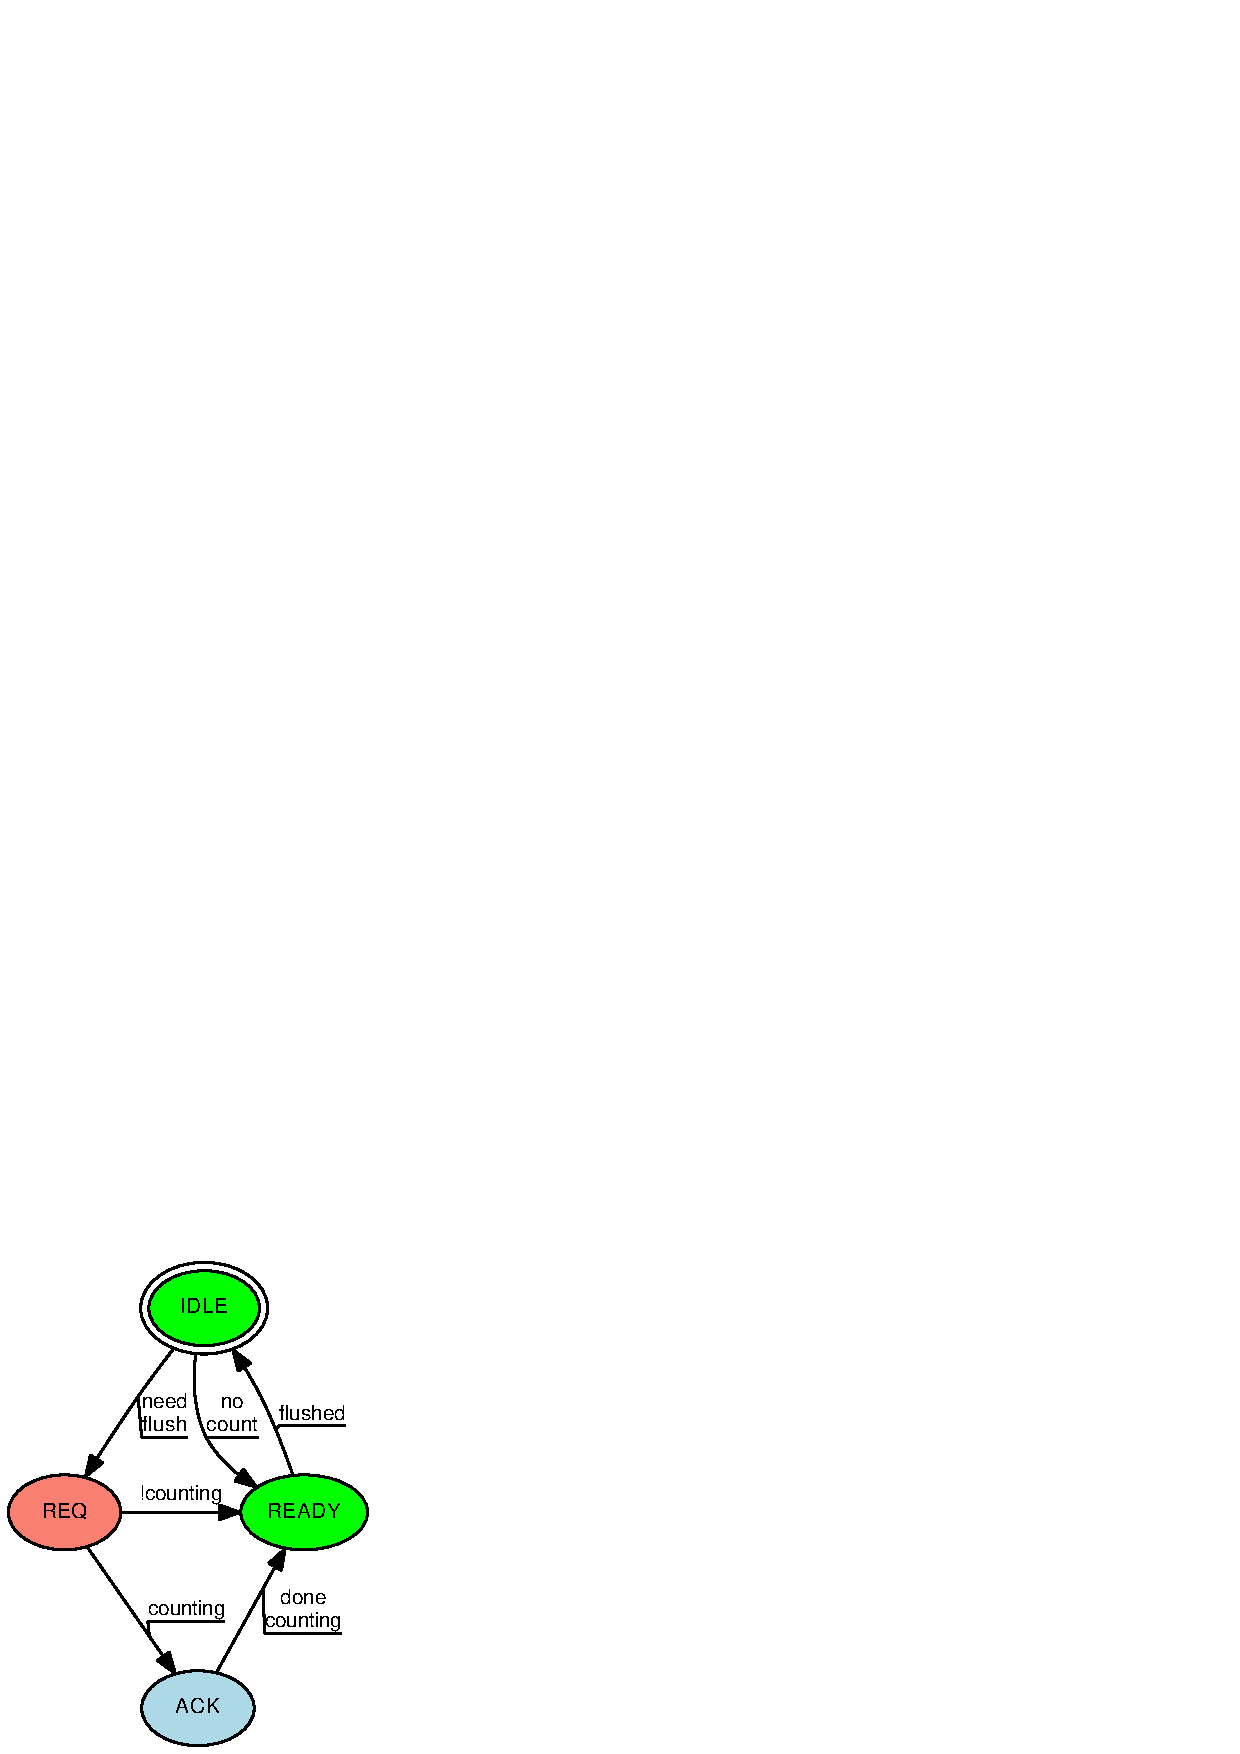
\includegraphics{count/sig-theft}}
\caption{Signal-Theft State Machine}
\label{fig:count:Signal-Theft State Machine}
\end{figure}

The state machine starts out in the IDLE state, and when \co{add_count()}
or \co{sub_count()} find that the combination of the local thread's count
and the global count cannot accommodate the request, the corresponding
slowpath sets each thread's \co{theft} state to REQ (unless that thread
has no count, in which case it transitions directly to READY).
Only the slowpath, which holds the \co{gblcnt_mutex} lock, is permitted to
transition from the IDLE state, as indicated by the green color.\footnote{
	For those with black-and-white versions of this book,
	IDLE and READY are green, REQ is red, and ACK is blue.}
The slowpath then sends a signal to each thread, and the corresponding
signal handler checks the corresponding thread's \co{theft} and
\co{counting} variables.
If the \co{theft} state is not REQ, then the signal handler is not
permitted to change the state, and therefore simply returns.
Otherwise, if the \co{counting} variable is set, indicating that
the current thread's fastpath is in progress, the signal handler
sets the \co{theft} state to ACK, otherwise to READY\@.

If the \co{theft} state is ACK,
only the fastpath is permitted to change
the \co{theft} state, as indicated by the blue color.
When the fastpath completes, it sets the \co{theft} state to READY\@.

Once the slowpath sees a thread's \co{theft} state is READY, the
slowpath is permitted to steal that thread's count.
The slowpath then sets that thread's \co{theft} state to IDLE\@.

\QuickQuizSeries{%
\QuickQuizB{
	In Figure~\ref{fig:count:Signal-Theft State Machine}, why is
	the REQ \co{theft} state colored red?
}\QuickQuizAnswerB{
	To indicate that only the fastpath is permitted to change the
	\co{theft} state, and that if the thread remains in this
	state for too long, the thread running the slowpath will
	resend the POSIX signal.
}\QuickQuizEndB
%
\QuickQuizE{
	In Figure~\ref{fig:count:Signal-Theft State Machine}, what is
	the point of having separate REQ and ACK \co{theft} states?
	Why not simplify the state machine by collapsing
	them into a single REQACK state?
	Then whichever of the signal handler or the fastpath gets there
	first could set the state to READY\@.
}\QuickQuizAnswerE{
	Reasons why collapsing the REQ and ACK states would be a very
	bad idea include:
	\begin{enumerate}
	\item	The slowpath uses the REQ and ACK states to determine
		whether the signal should be retransmitted.
		If the states were collapsed, the slowpath would have
		no choice but to send redundant signals, which would
		have the unhelpful effect of needlessly slowing down
		the fastpath.
	\item	The following race would result:
		\begin{enumerate}
		\item	The slowpath sets a given thread's state to REQACK.
		\item	That thread has just finished its fastpath, and
			notes the REQACK state.
		\item	The thread receives the signal, which also notes
			the REQACK state, and, because there is no fastpath
			in effect, sets the state to READY\@.
		\item	The slowpath notes the READY state, steals the
			count, and sets the state to IDLE, and completes.
		\item	The fastpath sets the state to READY, disabling
			further fastpath execution for this thread.
		\end{enumerate}
		The basic problem here is that the combined REQACK state
		can be referenced by both the signal handler and the
		fastpath.
		The clear separation maintained by the four-state
		setup ensures orderly state transitions.
	\end{enumerate}
	That said, you might well be able to make a three-state setup
	work correctly.
	If you do succeed, compare carefully to the four-state setup.
	Is the three-state solution really preferable, and why or why not?
}\QuickQuizEndE
}

\subsection{Signal-Theft Limit Counter Implementation}
\label{sec:count:Signal-Theft Limit Counter Implementation}

\begin{fcvref}[ln:count:count_lim_sig:data]
Listing~\ref{lst:count:Signal-Theft Limit Counter Data}
(\path{count_lim_sig.c})
shows the data structures used by the signal-theft based counter
implementation.
\Clnrefrange{value:b}{value:e} define the states and values
for the per-thread theft state machine
described in the preceding section.
\Clnrefrange{var:b}{var:e} are similar to earlier implementations,
with the addition of
lines~\lnref{maxp} and~\lnref{theftp} to allow remote access to a
thread's \co{countermax}
and \co{theft} variables, respectively.
\end{fcvref}

\begin{listing}[tbp]
\input{CodeSamples/count/count_lim_sig@data.fcv}
\caption{Signal-Theft Limit Counter Data}
\label{lst:count:Signal-Theft Limit Counter Data}
\end{listing}

\begin{fcvref}[ln:count:count_lim_sig:migration:globalize]
Listing~\ref{lst:count:Signal-Theft Limit Counter Value-Migration Functions}
shows the functions responsible for migrating counts between per-thread
variables and the global variables.
\Clnrefrange{b}{e} show \co{globalize_count()},
which is identical to earlier
implementations.
\end{fcvref}
\begin{fcvref}[ln:count:count_lim_sig:migration:flush_sig]
\Clnrefrange{b}{e} show \co{flush_local_count_sig()},
which is the signal
handler used in the theft process.
Lines~\lnref{check:REQ} and~\lnref{return:n} check to see if
the \co{theft} state is REQ, and, if not
returns without change.
Line~\lnref{mb:1} executes a memory barrier to ensure that the sampling of the
theft variable happens before any change to that variable.
Line~\lnref{set:ACK} sets the \co{theft} state to ACK, and, if
line~\lnref{check:fast} sees that
this thread's fastpaths are not running, line~\lnref{set:READY} sets the \co{theft}
state to READY\@.
\end{fcvref}

\begin{listing}[tbp]
\input{CodeSamples/count/count_lim_sig@migration.fcv}
\caption{Signal-Theft Limit Counter Value-Migration Functions}
\label{lst:count:Signal-Theft Limit Counter Value-Migration Functions}
\end{listing}

\QuickQuiz{
	In \cref{lst:count:Signal-Theft Limit Counter Value-Migration Functions}'s
	function \co{flush_local_count_sig()}, why are there
	\co{READ_ONCE()} and \co{WRITE_ONCE()} wrappers around
	the uses of the
	\co{theft} per-thread variable?
}\QuickQuizAnswer{
	\begin{fcvref}[ln:count:count_lim_sig:migration:flush_sig]
	The first one (on line~\lnref{check:REQ}) can be argued to be unnecessary.
	The last two (lines~\lnref{set:ACK} and~\lnref{set:READY}) are important.
	If these are removed, the compiler would be within its rights
	to rewrite \clnrefrange{set:ACK}{set:READY} as follows:
	\end{fcvref}

\begin{VerbatimN}[firstnumber=14]
theft = THEFT_READY;
if (counting) {
	theft = THEFT_ACK;
}
\end{VerbatimN}

	This would be fatal, as the slowpath might see the transient
	value of \co{THEFT_READY}, and start stealing before the
	corresponding thread was ready.
}\QuickQuizEnd

\begin{fcvref}[ln:count:count_lim_sig:migration:flush]
\Clnrefrange{b}{e} show \co{flush_local_count()}, which is called from the
slowpath to flush all threads' local counts.
The loop spanning
\clnrefrange{loop:b}{loop:e} advances the \co{theft} state for each
thread that has local count, and also sends that thread a signal.
Line~\lnref{skip} skips any non-existent threads.
Otherwise, line~\lnref{checkmax} checks to see if the current thread holds any local
count, and, if not, line~\lnref{READY} sets the thread's \co{theft} state to READY
and line~\lnref{next} skips to the next thread.
Otherwise, line~\lnref{REQ} sets the thread's \co{theft} state to REQ and
line~\lnref{signal} sends the thread a signal.
\end{fcvref}

\QuickQuizSeries{%
\QuickQuizB{
	In Listing~\ref{lst:count:Signal-Theft Limit Counter Value-Migration Functions},
	why is it safe for
        line~\ref{ln:count:count_lim_sig:migration:flush:checkmax}
        to directly access the other thread's
	\co{countermax} variable?
}\QuickQuizAnswerB{
	Because the other thread is not permitted to change the value
	of its \co{countermax} variable unless it holds the
	\co{gblcnt_mutex} lock.
	But the caller has acquired this lock, so it is not possible
	for the other thread to hold it, and therefore the other thread
	is not permitted to change its \co{countermax} variable.
	We can therefore safely access it---but not change it.
}\QuickQuizEndB
%
\QuickQuizM{
	In Listing~\ref{lst:count:Signal-Theft Limit Counter Value-Migration Functions},
	why doesn't
        line~\ref{ln:count:count_lim_sig:migration:flush:signal}
        check for the current thread sending itself
	a signal?
}\QuickQuizAnswerM{
	There is no need for an additional check.
	The caller of \co{flush_local_count()} has already invoked
	\co{globalize_count()}, so the check on
	line~\ref{ln:count:count_lim_sig:migration:flush:checkmax}
	will have succeeded, skipping the later \co{pthread_kill()}.
}\QuickQuizEndM
%
\QuickQuizE{
	The code shown in
	\cref{lst:count:Signal-Theft Limit Counter Data,%
	lst:count:Signal-Theft Limit Counter Value-Migration Functions}
	works with \GCC\ and POSIX\@.
	What would be required to make it also conform to the ISO C standard?
}\QuickQuizAnswerE{
	The \co{theft} variable must be of type \co{sig_atomic_t}
	to guarantee that it can be safely shared between the signal
	handler and the code interrupted by the signal.
}\QuickQuizEndE
}

\begin{fcvref}[ln:count:count_lim_sig:migration:flush]
The loop spanning \clnrefrange{loop2:b}{loop2:e} waits until each
thread reaches READY state,
then steals that thread's count.
\Clnrefrange{skip:nonexist}{next2} skip any non-existent threads,
and the loop spanning
\clnrefrange{loop3:b}{loop3:e} waits until the current
thread's \co{theft} state becomes READY\@.
Line~\lnref{block} blocks for a millisecond to avoid priority-inversion problems,
and if line~\lnref{check:REQ} determines that the thread's signal has not yet arrived,
line~\lnref{signal2} resends the signal.
Execution reaches line~\lnref{thiev:b} when the thread's \co{theft} state becomes
READY, so \clnrefrange{thiev:b}{thiev:e} do the thieving.
Line~\lnref{IDLE} then sets the thread's \co{theft} state back to IDLE\@.
\end{fcvref}

\QuickQuiz{
	In Listing~\ref{lst:count:Signal-Theft Limit Counter Value-Migration Functions},
        why does line~\ref{ln:count:count_lim_sig:migration:flush:signal2}
        resend the signal?
}\QuickQuizAnswer{
	Because many operating systems over several decades have
	had the property of losing the occasional signal.
	Whether this is a feature or a bug is debatable, but
	irrelevant.
	The obvious symptom from the user's viewpoint will not be
	a kernel bug, but rather a user application hanging.

	\emph{Your} user application hanging!
}\QuickQuizEnd

\begin{fcvref}[ln:count:count_lim_sig:migration:balance]
\Clnrefrange{b}{e} show \co{balance_count()}, which is similar to that of
earlier examples.
\end{fcvref}

\begin{listing}[tbp]
\input{CodeSamples/count/count_lim_sig@add.fcv}
\caption{Signal-Theft Limit Counter Add Function}
\label{lst:count:Signal-Theft Limit Counter Add Function}
\end{listing}

\begin{listing}[tb]
\input{CodeSamples/count/count_lim_sig@sub.fcv}
\caption{Signal-Theft Limit Counter Subtract Function}
\label{lst:count:Signal-Theft Limit Counter Subtract Function}
\end{listing}

\begin{fcvref}[ln:count:count_lim_sig:add]
Listing~\ref{lst:count:Signal-Theft Limit Counter Add Function}
shows the \co{add_count()} function.
The fastpath spans \clnrefrange{fast:b}{return:fs}, and the slowpath
\clnrefrange{acquire}{return:ss}.
Line~\lnref{fast:b} sets the per-thread \co{counting} variable to 1 so that
any subsequent signal handlers interrupting this thread will
set the \co{theft} state to ACK rather than READY, allowing this
fastpath to complete properly.
Line~\lnref{barrier:1} prevents the compiler from reordering any of the fastpath body
to precede the setting of \co{counting}.
Lines~\lnref{check:b} and~\lnref{check:e} check to see
if the per-thread data can accommodate
the \co{add_count()} and if there is no ongoing theft in progress,
and if so line~\lnref{add:f} does the fastpath addition and
line~\lnref{fasttaken} notes that
the fastpath was taken.

In either case, line~\lnref{barrier:2} prevents the compiler from reordering the
fastpath body to follow line~\lnref{clearcnt}, which permits any subsequent signal
handlers to undertake theft.
Line~\lnref{barrier:3} again disables compiler reordering, and then
line~\lnref{check:ACK}
checks to see if the signal handler deferred the \co{theft}
state-change to READY, and, if so, line~\lnref{mb} executes a memory
barrier to ensure that any CPU that sees line~\lnref{READY} setting state to
READY also sees the effects of line~\lnref{add:f}.
If the fastpath addition at line~\lnref{add:f} was executed, then
line~\lnref{return:fs} returns
success.
\end{fcvref}

\begin{listing}[tbp]
\input{CodeSamples/count/count_lim_sig@read.fcv}
\caption{Signal-Theft Limit Counter Read Function}
\label{lst:count:Signal-Theft Limit Counter Read Function}
\end{listing}

\begin{fcvref}[ln:count:count_lim_sig:add]
Otherwise, we fall through to the slowpath starting at line~\lnref{acquire}.
The structure of the slowpath is similar to those of earlier examples,
so its analysis is left as an exercise to the reader.
\end{fcvref}
Similarly, the structure of \co{sub_count()} on
Listing~\ref{lst:count:Signal-Theft Limit Counter Subtract Function}
is the same
as that of \co{add_count()}, so the analysis of \co{sub_count()} is also
left as an exercise for the reader, as is the analysis of
\co{read_count()} in
Listing~\ref{lst:count:Signal-Theft Limit Counter Read Function}.

\begin{listing}[tbp]
\input{CodeSamples/count/count_lim_sig@initialization.fcv}
\caption{Signal-Theft Limit Counter Initialization Functions}
\label{lst:count:Signal-Theft Limit Counter Initialization Functions}
\end{listing}

\begin{fcvref}[ln:count:count_lim_sig:initialization:init]
\Clnrefrange{b}{e} of
Listing~\ref{lst:count:Signal-Theft Limit Counter Initialization Functions}
show \co{count_init()}, which set up \co{flush_local_count_sig()}
as the signal handler for \co{SIGUSR1},
enabling the \co{pthread_kill()} calls in \co{flush_local_count()}
to invoke \co{flush_local_count_sig()}.
The code for thread registry and unregistry is similar to that of
earlier examples, so its analysis is left as an exercise for the
reader.
\end{fcvref}

\subsection{Signal-Theft Limit Counter Discussion}

The signal-theft implementation runs more than eight times as fast as the
atomic implementation on my six-core x86 laptop.
Is it always preferable?

The signal-theft implementation would be vastly preferable on Pentium-4
systems, given their slow atomic instructions, but the old 80386-based
Sequent Symmetry systems would do much better with the shorter path
length of the atomic implementation.
However, this increased update-side performance comes at the
prices of higher read-side overhead: Those POSIX signals are not free.
If ultimate performance is of the essence, you will need to measure
them both on the system that your application is to be deployed on.

\QuickQuiz{
	Not only are POSIX signals slow, sending one to each thread
	simply does not scale.
	What would you do if you had (say) 10,000 threads and needed
	the read side to be fast?
}\QuickQuizAnswer{
	One approach is to use the techniques shown in
	Section~\ref{sec:count:Eventually Consistent Implementation},
	summarizing an approximation to the overall counter value in
	a single variable.
	Another approach would be to use multiple threads to carry
	out the reads, with each such thread interacting with a
	specific subset of the updating threads.
}\QuickQuizEnd

This is but one reason why high-quality APIs are so important:
they permit implementations to be changed as required by ever-changing
hardware performance characteristics.

\QuickQuiz{
	What if you want an exact limit counter to be exact only for
	its lower limit, but to allow the upper limit to be inexact?
}\QuickQuizAnswer{
	One simple solution is to overstate the upper limit by the
	desired amount.
	The limiting case of such overstatement results in the
	upper limit being set to the largest value that the counter is
	capable of representing.
}\QuickQuizEnd

\subsection{Applying Exact Limit Counters}
\label{sec:count:Applying Exact Limit Counters}

Although the exact limit counter implementations presented in this
section can be very useful, they are not much help if the counter's value
remains near zero at all times, as it might when counting the number
of outstanding accesses to an I/O device.
The high overhead of such near-zero counting is especially painful
given that we normally don't care how many references there are.
As noted in the removable I/O device access-count problem posed by
\QuickQuizRef{\QcountQIOcnt},
the number of accesses is irrelevant except in those rare cases when
someone is actually trying to remove the device.

One simple solution to this problem is to add a large ``bias''
(for example, one billion) to the
counter in order to ensure that the value is far enough from zero that
the counter can operate efficiently.
When someone wants to remove the device, this bias is subtracted from
the counter value.
Counting the last few accesses will be quite inefficient,
but the important point is that the many prior accesses will have been
counted at full speed.

\QuickQuiz{
	What else had you better have done when using a biased counter?
}\QuickQuizAnswer{
	You had better have set the upper limit to be large enough
	accommodate the bias, the expected maximum number of accesses,
	and enough ``slop'' to allow the counter to work efficiently
	even when the number of accesses is at its maximum.
}\QuickQuizEnd

Although a biased counter can be quite helpful and useful, it is only a
partial solution to the removable I/O device access-count problem
called out on
page~\pageref{chp:Counting}.
When attempting to remove a device, we must not only know the precise
number of current I/O accesses, we also need to prevent any future
accesses from starting.
One way to accomplish this is to read-acquire a reader-writer lock
when updating the counter, and to write-acquire that same reader-writer
lock when checking the counter.
Code for doing I/O might be as follows:

\begin{fcvlabel}[ln:count:inline:I/O]
\begin{VerbatimN}[commandchars=\\\[\]]
read_lock(&mylock);		\lnlbl[acq]
if (removing) {			\lnlbl[check]
	read_unlock(&mylock);	\lnlbl[rel1]
	cancel_io();		\lnlbl[cancel]
} else {
	add_count(1);		\lnlbl[inc]
	read_unlock(&mylock);	\lnlbl[rel2]
	do_io();		\lnlbl[do]
	sub_count(1);		\lnlbl[dec]
}
\end{VerbatimN}
\end{fcvlabel}

\begin{fcvref}[ln:count:inline:I/O]
Line~\lnref{acq} read-acquires the lock, and either
line~\lnref{rel1} or~\lnref{rel2} releases it.
Line~\lnref{check} checks to see if the device is being removed, and, if so,
line~\lnref{rel1} releases the lock and
line~\lnref{cancel} cancels the I/O, or takes whatever
action is appropriate given that the device is to be removed.
Otherwise, line~\lnref{inc} increments the access count,
line~\lnref{rel2} releases the
lock, line~\lnref{do} performs the I/O, and
line~\lnref{dec} decrements the access count.
\end{fcvref}

\QuickQuiz{
	This is ridiculous!
	We are \emph{read}-acquiring a reader-writer lock to
	\emph{update} the counter?
	What are you playing at???
}\QuickQuizAnswer{
	Strange, perhaps, but true!
	Almost enough to make you think that the name
	``reader-writer lock'' was poorly chosen, isn't it?
}\QuickQuizEnd

The code to remove the device might be as follows:

\begin{fcvlabel}[ln:count:inline:remove]
\begin{VerbatimN}[commandchars=\\\[\]]
write_lock(&mylock);		\lnlbl[acq]
removing = 1;			\lnlbl[note]
sub_count(mybias);
write_unlock(&mylock);		\lnlbl[rel]
while (read_count() != 0) {	\lnlbl[loop:b]
	poll(NULL, 0, 1);
}				\lnlbl[loop:e]
remove_device();		\lnlbl[remove]
\end{VerbatimN}
\end{fcvlabel}

\begin{fcvref}[ln:count:inline:remove]
Line~\lnref{acq} write-acquires the lock and
line~\lnref{rel} releases it.
Line~\lnref{note} notes that the device is being removed, and the loop spanning
\clnrefrange{loop:b}{loop:e} waits for any I/O operations to complete.
Finally, line~\lnref{remove} does any additional processing needed to prepare for
device removal.
\end{fcvref}

\QuickQuiz{
	What other issues would need to be accounted for in a real system?
}\QuickQuizAnswer{
	A huge number!

	Here are a few to start with:

	\begin{enumerate}
	\item	There could be any number of devices, so that the
		global variables are inappropriate, as are the
		lack of arguments to functions like \co{do_io()}.
	\item	Polling loops can be problematic in real systems,
		wasting CPU time and energy.
		In many cases, an event-driven design is far better,
		for example, where the last completing I/O wakes up the
		device-removal thread.
	\item	The I/O might fail, and so \co{do_io()} will likely
		need a return value.
	\item	If the device fails, the last I/O might never complete.
		In such cases, there might need to be some sort of
		timeout to allow error recovery.
	\item	Both \co{add_count()} and \co{sub_count()} can
		fail, but their return values are not checked.
	\item	Reader-writer locks do not scale well.
		One way of avoiding the high read-acquisition costs
		of reader-writer locks is presented in
		\cref{chp:Locking,chp:Deferred Processing}.
	\end{enumerate}
}\QuickQuizEnd

\section{Parallel Counting Discussion}
\label{sec:count:Parallel Counting Discussion}
%
\epigraph{This idea that there is generality in the specific is of
	  far-reaching importance.}
	 {\emph{Douglas R. Hofstadter}}

This chapter has presented the reliability, performance, and
scalability problems with traditional counting primitives.
The C-language \co{++} operator is not guaranteed to function reliably in
multithreaded code, and atomic operations to a single variable neither
perform nor scale well.
This chapter therefore presented a number of counting algorithms that
perform and scale extremely well in certain special cases.

It is well worth reviewing the lessons from these counting algorithms.
To that end,
Section~\ref{sec:count:Parallel Counting Performance}
summarizes performance and scalability,
Section~\ref{sec:count:Parallel Counting Specializations}
discusses the need for specialization,
and finally,
Section~\ref{sec:count:Parallel Counting Lessons}
enumerates lessons learned and calls attention to later chapters that
will expand on these lessons.

\begin{table*}
\rowcolors{4}{}{lightgray}
\renewcommand*{\arraystretch}{1.1}
\small
\centering
\newcommand{\NA}{\cellcolor{white}}
\begin{tabular}{lrcS[table-format=2.1]S[table-format=3.0]S[table-format=4.0]
		  S[table-format=6.0]S[table-format=6.0]}
	\toprule
	\multirow{2}{*}{\begin{picture}(60,15)(0,-3)\put(0,0){Algorithm}
			\put(14,-10){(\path{count_*.c})}\end{picture}} &
	    & \multirow{2}{*}{\begin{picture}(6,50)(0,-24)\rotatebox{90}{Exact?}\end{picture}} &
		\multicolumn{1}{c}{\multirow{2}{*}{\begin{picture}(30,15)(0,-3)
			\put(0,0){Updates}\put(15,-10){(ns)}\end{picture}}} &
			\multicolumn{4}{c}{Reads (ns)} \\
	\cmidrule{5-8}
	    & Section & & &
				   \multicolumn{1}{r}{1 CPU} &
				      \multicolumn{1}{r}{8 CPUs} &
					 \multicolumn{1}{r}{64 CPUs} &
					    \multicolumn{1}{r}{420 CPUs} \\
		\midrule
		\path{stat} & \ref{sec:count:Array-Based Implementation} & \NA &
		 6.3 & 294 & 303   & 315     &    612 \\
	\path{stat_eventual} & \ref{sec:count:Eventually Consistent Implementation} & \NA &
		 6.4 &   1 &   1   &   1     &      1 \\
	\path{end} & \ref{sec:count:Per-Thread-Variable-Based Implementation} & \NA &
		 2.9 & 301 & 6 309 & 147 594 & 239 683 \\
	\path{end_rcu} & \ref{sec:together:RCU and Per-Thread-Variable-Based Statistical Counters} & \NA &
		 2.9 & 454 &   481 &     508 &   2 317 \\
	\midrule
	\path{lim} & \ref{sec:count:Simple Limit Counter Implementation} &
		N &  3.2 & 435 & 6 678 & 156 175 & 239 422 \\
	\path{lim_app} & \ref{sec:count:Approximate Limit Counter Implementation} &
		N &  2.4 & 485 & 7 041 & 173 108 & 239 682 \\
	\path{lim_atomic} & \ref{sec:count:Atomic Limit Counter Implementation} &
		Y & 19.7 & 513 & 7 085 & 199 957 & 239 450 \\
	\path{lim_sig} & \ref{sec:count:Signal-Theft Limit Counter Implementation} &
		Y &  4.7 & 519 & 6 805 & 120 000 & 238 811 \\
	\bottomrule
\end{tabular}
\caption{Statistical/Limit Counter Performance on x86}
\label{tab:count:Statistical/Limit Counter Performance on x86}
\end{table*}

\subsection{Parallel Counting Performance}
\label{sec:count:Parallel Counting Performance}

The top half of \cref{tab:count:Statistical/Limit Counter Performance on x86}
shows the performance of the four parallel statistical counting
algorithms.
All four algorithms provide near-perfect linear scalability for updates.
The per-thread-variable implementation (\path{count_end.c})
is significantly faster on
updates than the array-based implementation
(\path{count_stat.c}), but is slower at reads on large numbers of core,
and suffers severe lock contention when there are many parallel readers.
This contention can be addressed using the deferred-processing
techniques introduced in
Chapter~\ref{chp:Deferred Processing},
as shown on the \path{count_end_rcu.c} row of
\cref{tab:count:Statistical/Limit Counter Performance on x86}.
Deferred processing also shines on the \path{count_stat_eventual.c} row,
courtesy of eventual consistency.

\QuickQuizSeries{%
\QuickQuizB{
	On the \path{count_stat.c} row of
	\cref{tab:count:Statistical/Limit Counter Performance on x86},
	we see that the read-side scales linearly with the number of
	threads.
	How is that possible given that the more threads there are,
	the more per-thread counters must be summed up?
}\QuickQuizAnswerB{
	The read-side code must scan the entire fixed-size array, regardless
	of the number of threads, so there is no difference in performance.
	In contrast, in the last two algorithms, readers must do more
	work when there are more threads.
	In addition, the last two algorithms interpose an additional
	level of indirection because they map from integer thread ID
	to the corresponding \co{__thread} variable.
}\QuickQuizEndB
%
\QuickQuizE{
	Even on the fourth row of
	\cref{tab:count:Statistical/Limit Counter Performance on x86},
	the read-side performance of these statistical counter
	implementations is pretty horrible.
	So why bother with them?
}\QuickQuizAnswerE{
	``Use the right tool for the job.''

	As can be seen from
	Figure~\ref{fig:count:Atomic Increment Scalability on x86},
	single-variable atomic increment need not apply for any job
	involving heavy use of parallel updates.
	In contrast, the algorithms shown in the top half of
	\cref{tab:count:Statistical/Limit Counter Performance on x86}
	do an excellent job of handling update-heavy situations.
	Of course, if you have a read-mostly situation, you should
	use something else, for example, an eventually consistent design
	featuring a single atomically incremented
	variable that can be read out using a single load,
	similar to the approach used in
	Section~\ref{sec:count:Eventually Consistent Implementation}.
}\QuickQuizEndE
}

The bottom half of \cref{tab:count:Statistical/Limit Counter Performance on x86}
shows the performance of the parallel limit-counting algorithms.
Exact enforcement of the limits incurs a substantial update-side
performance penalty, although on this x86 system that penalty can be
reduced by substituting signals for atomic operations.
All of these implementations suffer from read-side lock contention
in the face of concurrent readers.

\QuickQuizSeries{%
\QuickQuizB{
	Given the performance data shown in the bottom half of
	\cref{tab:count:Statistical/Limit Counter Performance on x86},
	we should always prefer signals over atomic operations, right?
}\QuickQuizAnswerB{
	That depends on the workload.
	Note that on a 64-core system, you need more than
	one hundred non-atomic operations (with roughly
	a 40-nanosecond performance gain) to make up for even one
	signal (with almost a 5-\emph{microsecond} performance loss).
	Although there are no shortage of workloads with far greater
	read intensity, you will need to consider your particular
	workload.

	In addition, although memory barriers have historically been
	expensive compared to ordinary instructions, you should
	check this on the specific hardware you will be running.
	The properties of computer hardware do change over time,
	and algorithms must change accordingly.
}\QuickQuizEndB
%
\QuickQuizE{
	Can advanced techniques be applied to address the lock
	contention for readers seen in the bottom half of
	\cref{tab:count:Statistical/Limit Counter Performance on x86}?
}\QuickQuizAnswerE{
	One approach is to give up some update-side performance, as is
	done with scalable non-zero indicators
	(SNZI)~\cite{FaithEllen:2007:SNZI}.
	There are a number of other ways one might go about this, and these
	are left as exercises for the reader.
	Any number of approaches that apply hierarchy, which replace
	frequent global-lock acquisitions with local lock acquisitions
	corresponding to lower levels of the hierarchy, should work quite well.
}\QuickQuizEndE
}

In short, this chapter has demonstrated a number of counting algorithms
that perform and scale extremely well in a number of special cases.
But must our parallel counting be confined to special cases?
Wouldn't it be better to have a general algorithm that operated
efficiently in all cases?
The next section looks at these questions.

\subsection{Parallel Counting Specializations}
\label{sec:count:Parallel Counting Specializations}

The fact that these algorithms only work well in their respective special
cases might be considered a major problem with parallel programming in
general.
After all, the C-language \co{++} operator works just fine in single-threaded
code, and not just for special cases, but in general, right?

This line of reasoning does contain a grain of truth, but is in essence
misguided.
The problem is not parallelism as such, but rather scalability.
To understand this, first consider the C-language \co{++} operator.
The fact is that it does \emph{not} work in general, only for a restricted
range of numbers.
If you need to deal with 1,000-digit decimal numbers, the C-language \co{++}
operator will not work for you.

\QuickQuiz{
	The \co{++} operator works just fine for 1,000-digit numbers!
	Haven't you heard of operator overloading???
}\QuickQuizAnswer{
	In the C++ language, you might well be able to use \co{++}
	on a 1,000-digit number, assuming that you had access to a
	class implementing such numbers.
	But as of 2021, the C language does not permit operator overloading.
}\QuickQuizEnd

This problem is not specific to arithmetic.
Suppose you need to store and query data.
Should you use an ASCII file?
XML?
A relational database?
A linked list?
A dense array?
A B-tree?
A radix tree?
Or one of the plethora of other data
structures and environments that permit data to be stored and queried?
It depends on what you need to do, how fast you need it done, and how
large your data set is---even on sequential systems.

Similarly, if you need to count, your solution will depend on how large
of numbers you need to work with, how many CPUs need to be manipulating
a given number concurrently, how the number is to be used, and what
level of performance and scalability you will need.

Nor is this problem specific to software.
The design for a bridge meant to allow people to walk across a small brook
might be a simple as a single wooden plank.
But you would probably not use a plank to span the kilometers-wide mouth of
the Columbia River, nor would such a design be advisable for bridges
carrying concrete trucks.
In short, just as bridge design must change with increasing span and load,
so must software design change as the number of CPUs increases.
That said, it would be good to automate this process, so that the
software adapts to changes in hardware configuration and in workload.
There has in fact been some research into this sort of
automation~\cite{Appavoo03a,Soules03a}, and the Linux kernel does some
boot-time reconfiguration, including limited binary rewriting.
This sort of adaptation will become increasingly important as the
number of CPUs on mainstream systems continues to increase.

In short, as discussed in
Chapter~\ref{chp:Hardware and its Habits},
the laws of physics constrain parallel software just as surely as they
constrain mechanical artifacts such as bridges.
These constraints force specialization, though in the case of software
it might be possible to automate the choice of specialization to
fit the hardware and workload in question.

Of course, even generalized counting is quite specialized.
We need to do a great number of other things with computers.
The next section relates what we have learned from counters to
topics taken up later in this book.

\subsection{Parallel Counting Lessons}
\label{sec:count:Parallel Counting Lessons}

The opening paragraph of this chapter promised that our study of counting
would provide an excellent introduction to parallel programming.
This section makes explicit connections between the lessons from
this chapter and the material presented in a number of later chapters.

The examples in this chapter have shown that an important scalability
and performance tool is \emph{partitioning}.
The counters might be fully partitioned, as in the statistical counters
discussed in \cref{sec:count:Statistical Counters},
or partially partitioned as in the limit counters discussed in
\cref{sec:count:Approximate Limit Counters,%
sec:count:Exact Limit Counters}.
Partitioning will be considered in far greater depth in
\cref{cha:Partitioning and Synchronization Design},
and partial parallelization in particular in
\cref{sec:SMPdesign:Parallel Fastpath}, where it is called
\emph{parallel fastpath}.

\QuickQuiz{
	But if we are going to have to partition everything, why bother
	with shared-memory multithreading?
	Why not just partition the problem completely and run as
	multiple processes, each in its own address space?
}\QuickQuizAnswer{
	Indeed, multiple processes with separate address spaces can be
	an excellent way to exploit parallelism, as the proponents of
	the fork-join methodology and the Erlang language would be very
	quick to tell you.
	However, there are also some advantages to shared-memory parallelism:
	\begin{enumerate}
	\item	Only the most performance-critical portions of the
		application must be partitioned, and such portions
		are usually a small fraction of the application.
	\item	Although cache misses are quite slow compared to
		individual register-to-register instructions,
		they are typically considerably faster than
		inter-process-communication primitives, which in
		turn are considerably faster than things like
		TCP/IP networking.
	\item	Shared-memory multiprocessors are readily available
		and quite inexpensive, so, in stark contrast to the
		1990s, there is little cost penalty for use of
		shared-memory parallelism.
	\end{enumerate}
	As always, use the right tool for the job!
}\QuickQuizEnd

The partially partitioned counting algorithms used locking to
guard the global data, and locking is the subject of
Chapter~\ref{chp:Locking}.
In contrast, the partitioned data tended to be fully under the control of
the corresponding thread, so that no synchronization whatsoever was required.
This \emph{data ownership} will be introduced in
Section~\ref{sec:SMPdesign:Data Ownership}
and discussed in more detail in
Chapter~\ref{chp:Data Ownership}.

Because integer addition and subtraction are extremely cheap
compared to typical synchronization operations, achieving reasonable
scalability requires synchronization operations be used sparingly.
One way of achieving this is to batch the addition and subtraction
operations, so that a great many of these cheap operations are handled
by a single synchronization operation.
Batching optimizations of one sort or another are used by each of
the counting algorithms listed in
\cref{tab:count:Statistical/Limit Counter Performance on x86}.

Finally, the eventually consistent statistical counter discussed in
Section~\ref{sec:count:Eventually Consistent Implementation}
showed how deferring activity (in that case, updating the global
counter) can provide substantial performance and scalability benefits.
This approach allows common case code to use much cheaper synchronization
operations than would otherwise be possible.
Chapter~\ref{chp:Deferred Processing} will examine a number of additional
ways that deferral can improve performance, scalability, and even
real-time response.

Summarizing the summary:

\begin{enumerate}
\item	Partitioning promotes performance and scalability.
\item	Partial partitioning, that is, partitioning applied only to
	common code paths, works almost as well.
\item	Partial partitioning can be applied to code (as in
	Section~\ref{sec:count:Statistical Counters}'s statistical
	counters' partitioned updates and non-partitioned reads), but also
	across time (as in
	Section~\ref{sec:count:Approximate Limit Counters}'s and
	Section~\ref{sec:count:Exact Limit Counters}'s
	limit counters running fast when far from
	the limit, but slowly when close to the limit).
\item	Partitioning across time often batches updates locally
	in order to reduce the number of expensive global operations,
	thereby decreasing synchronization overhead, in turn
	improving performance and scalability.
	All the algorithms shown in
	\cref{tab:count:Statistical/Limit Counter Performance on x86}
	make heavy use of batching.
\item	Read-only code paths should remain read-only:  Spurious
	synchronization writes to shared memory kill performance
	and scalability, as seen in the \path{count_end.c} row of
	\cref{tab:count:Statistical/Limit Counter Performance on x86}.
\item	Judicious use of delay promotes performance and scalability, as
	seen in Section~\ref{sec:count:Eventually Consistent Implementation}.
\item	Parallel performance and scalability is usually a balancing act:
	Beyond a certain point, optimizing some code paths will degrade
	others.
	The \path{count_stat.c} and \path{count_end_rcu.c} rows of
	\cref{tab:count:Statistical/Limit Counter Performance on x86}
	illustrate this point.
\item	Different levels of performance and scalability will affect
	algorithm and data-structure design, as do a large number of
	other factors.
	\Cref{fig:count:Atomic Increment Scalability on x86}
	illustrates this point:  Atomic increment might be completely
	acceptable for a two-CPU system, but be completely inadequate for an
	eight-CPU system.
\end{enumerate}

\begin{figure}[tb]
\centering
\resizebox{3in}{!}{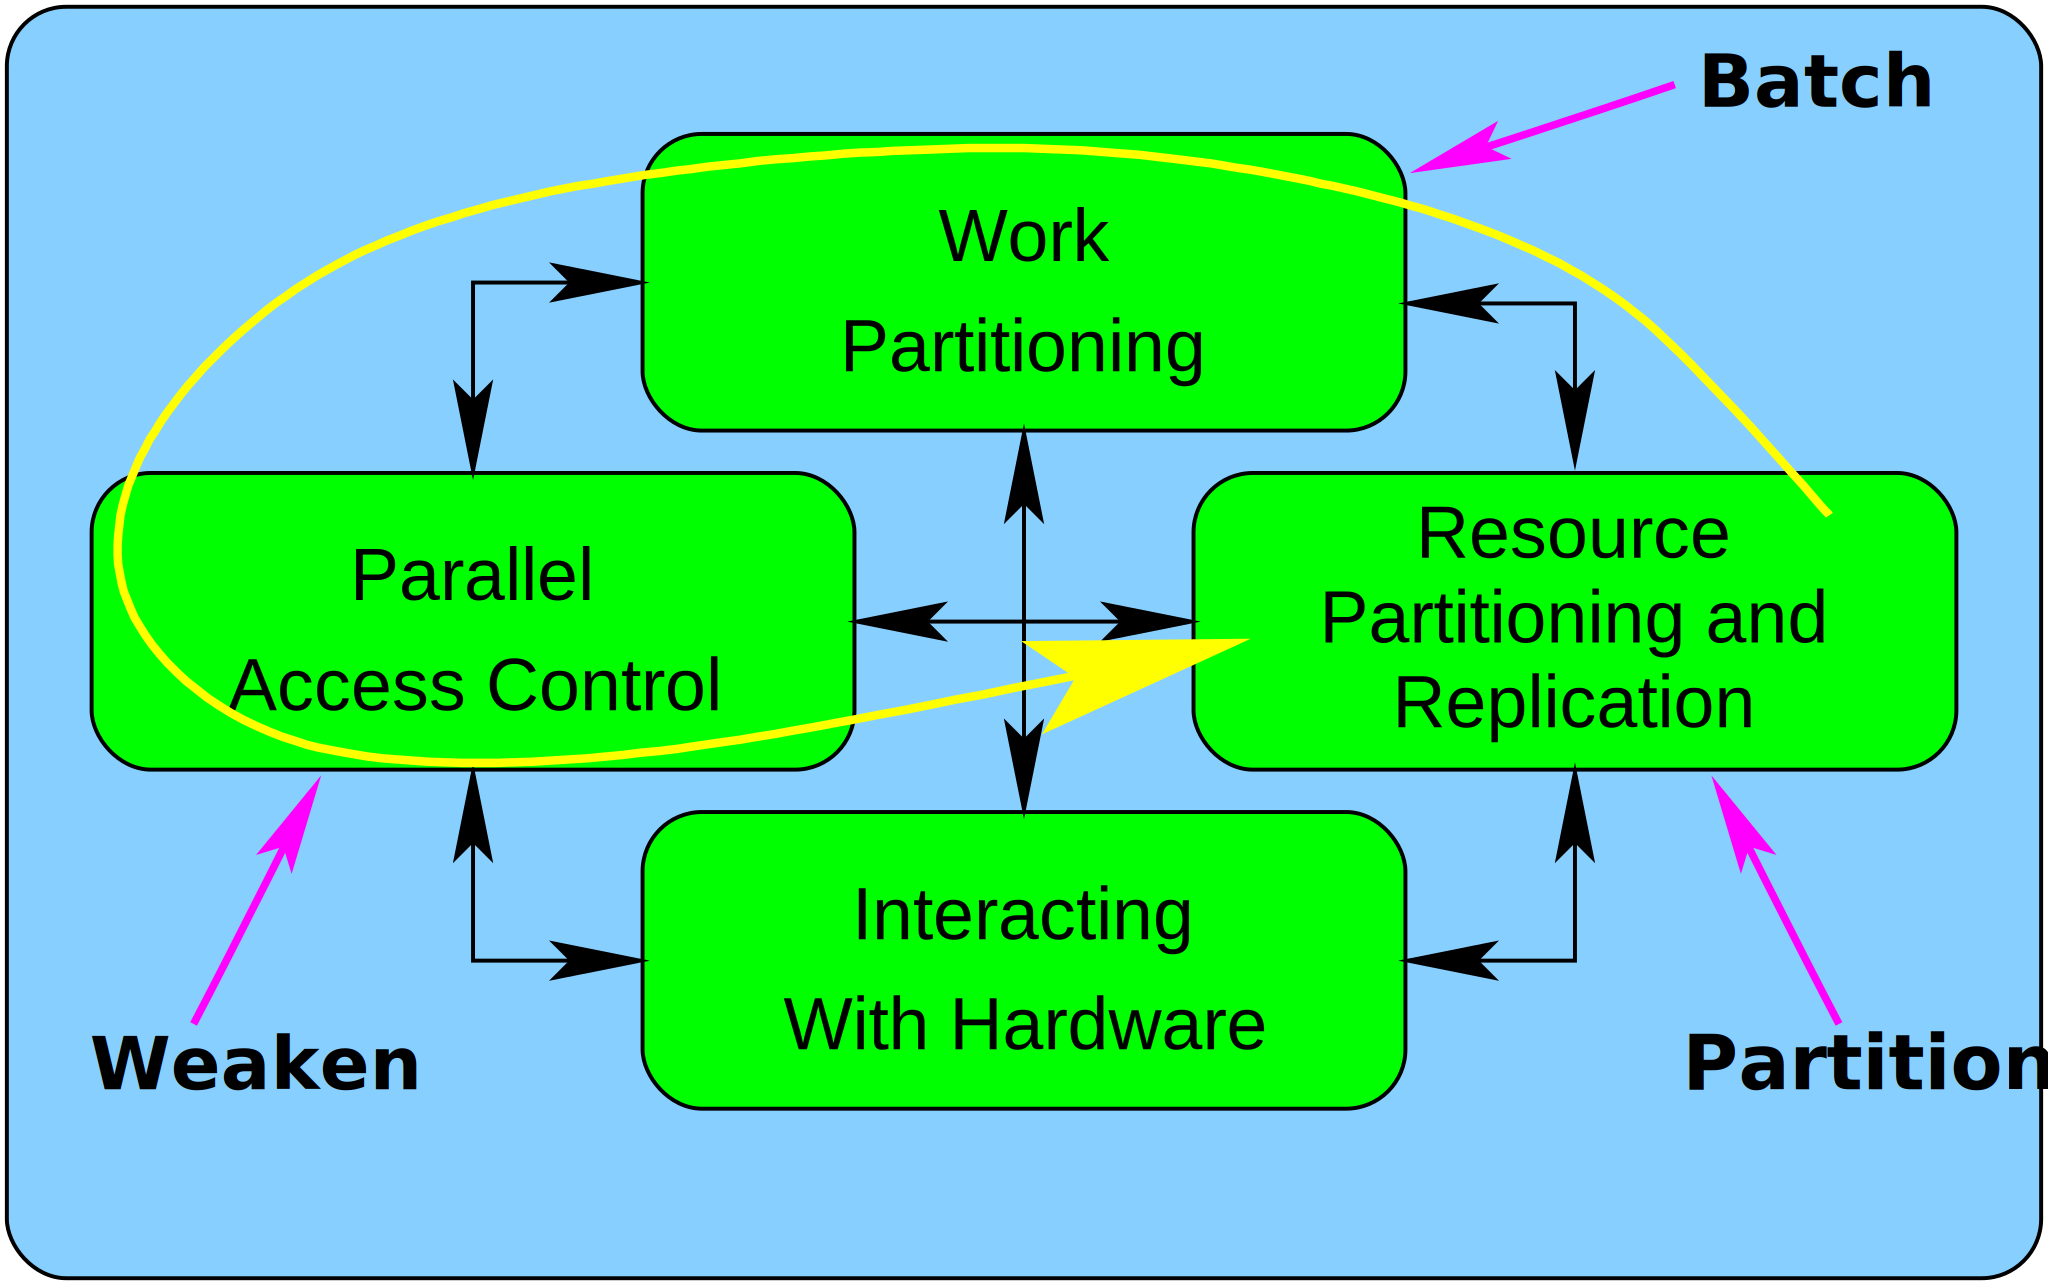
\includegraphics{count/FourTaskOrderOpt}}
\caption{Optimization and the Four Parallel-Programming Tasks}
\label{fig:count:Optimization and the Four Parallel-Programming Tasks}
\end{figure}

Summarizing still further, we have the ``big three'' methods of
increasing performance and scalability, namely
(1)~\emph{partitioning} over CPUs or threads,
(2)~\emph{batching} so that more work can be done by each expensive
synchronization operations, and
(3)~\emph{weakening} synchronization operations where feasible.
As a rough rule of thumb, you should apply these methods in this order,
as was noted earlier in the discussion of
Figure~\ref{fig:intro:Ordering of Parallel-Programming Tasks}
on
page~\pageref{fig:intro:Ordering of Parallel-Programming Tasks}.
The partitioning optimization applies to the
``Resource Partitioning and Replication'' bubble,
the batching optimization to the ``Work Partitioning'' bubble,
and the weakening optimization to the ``Parallel Access Control'' bubble,
as shown in
Figure~\ref{fig:count:Optimization and the Four Parallel-Programming Tasks}.
Of course, if you are using special-purpose hardware such as
digital signal processors (DSPs), field-programmable gate arrays (FPGAs),
or general-purpose graphical processing units (GPGPUs), you may need
to pay close attention to the ``Interacting With Hardware'' bubble
throughout the design process.
For example, the structure of a GPGPU's hardware threads and memory
connectivity might richly reward very careful partitioning
and batching design decisions.

In short, as noted at the beginning of this chapter, the simplicity
of counting have allowed us to explore many
fundamental concurrency issues without the distraction of
complex synchronization primitives or elaborate data structures.
Such synchronization primitives and data structures are covered
in later chapters.

\QuickQuizAnswersChp{qqzcount}
